% \begin{enumerate}
%     \item Theoretical Justification for Sensitivity-Constrained Training
%         \begin{itemize}
%           \item Neural Operators
%           \item Sensitivity-Constrained Neural Operators (SC-NO)
%           \item Theoretical Justification:
%             \begin{itemize}
%                 \item Assumptions and Notation
%                 \item Assumption 1 (Uniform Convergence of Gradients)
%                 \item Assumption 2 (Uniform Convergence of Solutions)
%                 \item Cost Functionals
%                 \item Improved Generalization
%                 \item Long-Term Prediction Stability
%                 \item Inversion Accuracy
%             \end{itemize}
%         \end{itemize}    
    
%     \item Data Generation
%         \begin{itemize}
%             \item Structure of the Input Function
%             \item Dataset Structure with True Sensitivities
%             \item Scaled Gaussian Random Field for Parameter Generation
%         \end{itemize}
    
%     \item PDE1: Advection-Diffusion Equation with Spatially Distributed Velocity Field
%         \begin{itemize}
%             \item Problem setup
%             \item Numerical Solver for the Advection-Diffusion Equation
%             \item Neural Operator Learning for the Advection-Diffusion Equation
%             \item Additional results for PDE1 (Tables 2 and 3; Figures 8 and 9)
%         \end{itemize}

%     \item PDE2: Turbulent Navier--Stokes Equations with Spalart--Allmaras Closure

%         \begin{itemize}
%             \item Problem setup
%             \item Numerical Solver for the Turbulent Navier--Stokes Equations
%             \item Neural Operator Learning for the Turbulent Navier--Stokes Equations
%             \item Adjoint-Based Sensitivity Computation for the Turbulent Navier--Stokes Equations
%             \item Additional results for PDE2 (Tables 4 and 5; Figures 10-12)
%         \end{itemize}

    
%     \item PDE3: 2D Shallow Water Equations for the Tohoku 2011 Tsunami
%         \begin{itemize}
%             \item Problem setup
%             \item Modeling Seafloor Deformation Using the Okada Dislocation Model
%             \item Finite Volume Method for Shallow Water Equations
%             \item Adjoint-Based Sensitivity Computation
%             \item Neural Operator Learning for the Shallow Water Equations
%             \item Mapping Between Fine Solver Mesh and Coarse Neural Operator Grid
%             \item Three-Stage Inversion Framework for Tsunami Source Reconstruction (Figures 17-20)
%             \item Additional results for PDE3 (Tables 6 and 7)
%         \end{itemize}

%     \item Applicability, Limitations, and Future Extensions
%     \item Performance Metrics
%     \item Experiments
%         \begin{itemize}
%           \item Forward Prediction
%           \item Inverse Inference via Optimization
%         \end{itemize}
%     \item Hyperparameters and Settings (Tables 8-10)
%     \item Computational Cost Analysis (Tables 11-13)
%     \item Figures \ref{fig:bed_elevation} to \ref{fig:gauge_timeseries}
% \end{enumerate}

% \newpage

% % %%%%%%%%%%%%%%%% MATERIALS AND METHODS %%%%%%%%%%%%%%%
% % \section{Methods}
This section contains a condensed overview of the neural operator architectures, PDEs, their numerical solution and adjoint calculations, experimental setup, Jacobian sampling, and inversion. Suppmentary materials expand on the details of each component.
\subsection{The SC-NO scheme:} 
Neural Operators (NOs) approximate solution operators for PDEs by learning mappings between function spaces \citep{lu2021learning, kovachki2023neural}. Given an input function \( a(\mathbf{x}, t, p) \)—for example, a spatial field such as an initial condition—NOs learn a parameterized operator \( \mathcal{G}_\theta \) such that \( u(\mathbf{x}, t, p) = \mathcal{G}_\theta(a)(\mathbf{x}, t, p) \), where \( \mathbf{x} \) denotes spatial coordinates, \( t \) denotes time, and \( p \) represents PDE parameters (e.g., viscosity, diffusion coefficients, or forcing magnitudes). The operator thus maps an input function over space--time--parameter domains to an output solution function; for instance, given bed elevation \( a(\mathbf{x}) \), the model predicts water height \( u(\mathbf{x}, t) \) across space and time. SC-NO extends standard NOs by incorporating sensitivity constraints, ensuring accurate gradient predictions alongside state values. The latent representation \( v_t(\mathbf{x}, t, p) \) evolves iteratively as
\( v_{t+1} = \sigma\!\left( \mathcal{K}_\theta(v_t) + \mathcal{L}_\theta(v_t) \right) \),
where \( \mathcal{K}_\theta \) is a nonlocal integral operator and \( \mathcal{L}_\theta \) is a local transformation. The sensitivity-regularized loss minimizes erdo you rors in both state predictions and their parameter sensitivities,
\( \mathcal{L} = \| u - u_{\theta} \|^2 + \lambda \left\| \nabla_{p} u - \nabla_{p} u_{\theta} \right\|^2 \),
where \( \nabla_{p} u \) denotes the gradient of the true solution with respect to the PDE parameters \( p \). Training data—including both solution fields and their sensitivities—are generated using a differentiable PDE solver, enabling consistent supervision of both \( u \) and \( \nabla_{p} u \). SC-NO ensures physics-consistent learning for parametric PDEs, enhancing generalization to unseen conditions. Figure~\ref{fig:sc_no_frame} illustrates the SC-NO framework. A detailed methodological description, along with the rigorous mathematical proof of these guarantees, is provided in Appendix~\ref{sec_sup_method}.


% SC-NOs structure
\begin{figure}[htbp]
    \centering
    \includegraphics[width=0.8\textwidth, trim={0 0 0 0}, clip]{Figuers/SC-NO_framwork.pdf}
    \caption{\scriptsize\textbf{Overview of the Sensitivity-Constrained Neural Operator Framework.} The process begins with input data, including initial states \( a(x, t, p) \) . A neural operator maps these inputs to predicted states \( u(x, t, p) \), while automatic differentiation computes the Jacobian \( \partial u / \partial p \). The framework optimizes a loss function that combines prediction loss \( L_u \) and sensitivity loss \( L_S \), ensuring accuracy and consistency with respect to parameters.}
    \label{fig:sc_no_frame}
\end{figure}



The proposed Sensitivity-Constrained Neural Operator framework is summarized in Figure~\ref{fig:sc_no_frame}. Building on neural operators' universal approximation capabilities, SC-NO incorporates stochastic Jacobian supervision into the training objective by combining the standard prediction loss with a sensitivity regularization term. In each minibatch, the model uses a randomly selected subset of entries from the full Jacobian rather than the entire tensor, and these subsets vary across training so that the model ultimately receives supervision over the full Jacobian without incurring its per-step computational cost. This design improves robustness and generalization to unseen conditions, enabling the model to learn the forward solution operator while simultaneously aligning with parameter sensitivities.

\subsection{Sensitivities through NOs:} 
Either a differentiable numerical model or its neural operator surrogate can compute sensitivities, namely the gradient (or Jacobian) of the output solution with respect to input parameters, forcings, and/or initial conditions. For neural operators, the simplest Jacobian computation is through automatic differentiation (AD), in which we write the forward mode on an AD-supporting platform like PyTorch, JAX, Julia, Tensorflow, etc., and the backward is automatically provided by the platform. We leverage the \texttt{torch.autograd.grad} functionality from PyTorch to efficiently compute Jacobians over different components of the output states, although the same can be provided using other platforms. For acceleration, a proprietary library can parallelize this computation over a minibatch of simulations and multiple output state values, with some cost in increased graphics processing unit (GPU) memory usage. However, AD can rapidly exhaust GPU memory for complex numerical solvers that require the solution of large linear systems or iterative procedures to resolve nonlinearities. In such cases, adjoint-based sensitivity analysis provides a more memory-efficient alternative, with computational cost comparable to a forward--adjoint solve, as described next. While finite-difference methods can be effective in low-dimensional settings, they are not applicable to the high-dimensional cases examined here.


\subsection{Numerical solutions to PDEs and Sensitivity calculations:}
All three PDEs are solved using custom-built, programmatically-differentiable numerical solvers to enable consistent forward simulation and sensitivity evaluation. For PDE1 (ADE) and PDE2 (RANS), the spatially discretized systems are cast as an ordinary differential equation in time and integrated using adaptive Runge-Kutta time stepping, leveraging parts of the \texttt{torchdiffeq} package. Sensitivities for PDE1 are obtained through automatic differentiation of the time integration (not the ``Optimize-then-Discretize" Adjoint offered by \texttt{torchdiffeq}), yielding exact gradients of the discretized dynamics with respect to spatially distributed inputs. For PDE2, sensitivities are computed using a discrete-time adjoint (\textit{Discretize-then-Optimize}) derived from a Lagrangian formulation of the time-discretized RANS system with Spalart–Allmaras closure, enabling efficient gradient evaluation with respect to initial conditions and forcing fields independent of parameter dimensionality.

For PDE3 (Shallow Water), we implemented a finite-volume solver on an unstructured triangular mesh and advance the coupled state variables using an adaptive second-order Heun scheme subject to a CFL stability condition. Numerical fluxes across cell interfaces are computed using the HLLC (Harten-Lax-van Leer-Contact) approximate Riemann solver, similar to the finite volume methods used before \citep{vogl2017high}. Just as for RANS, the corresponding adjoint system is constructed via a discrete-time Lagrangian formulation and solved by backward recursion that mirrors the forward time stepping. Local Jacobians of numerical fluxes and source terms are assembled at the cell level, and gradients with respect to bed topography are obtained by accumulating adjoint-weighted source sensitivities over time. This adjoint formulation computes full-field sensitivities at a cost comparable to a single forward–backward solve, enabling scalable inversion and forecasting for high-dimensional tsunami applications. The Tohoku tsunami case runs a 3,600-second simulation on an unstructured triangular mesh consisting of 308,001 cells and 154,598 nodes, ensuring mass conservation and allowing adaptive local refinement in coastal and impact regions. We use ETOPO 2022 at 30 Arc-Second resolution as initial bathymetry to cover the 1000 km × 1000 km simulation domain (Supplementary Figure \ref{fig:bed_elevation}). The solver has been validated by observed data, e.g., as shown in Supplementary Figure \ref{fig:tohoku_validation} for North Miyagi offshore GPS wave gauge (station 803, NOWPHAS network) in the 2011 Tohoku tsunami event. We have validated the solver on various other small and large events but data are not shown here as the solver is not the focus of this study. The solution and Jacobians are coarsened before training the neural operators.

\subsection{Jacobian sampling and its amortization in the training loop.}
Using reverse-mode differentiation, concurrent AI training can calculate the gradient $\partial u / \partial p$ where $p$ can reach billions or even trillions of parameters, but obtaining the Jacobian entries for many output points $u$ can still be expensive in terms of compute and GPU memory. We therefore sample only a subset of $u$ points in space for the last time point when forming the sensitivity loss. Crucially, the precomputed Jacobian is randomly resampled in every minibatch of the main surrogate training loop. In expectation, the sampled sensitivity loss provides an unbiased estimate of the full Jacobian loss, i.e., $\mathbb{E}[\mathcal{L}{\text{Jac}}^{\text{sampled}}] = \mathcal{L}{\text{Jac}}$. As training proceeds, different Jacobian directions are observed, so that the model effectively covers the full Jacobian space over time while maintaining a bounded per-iteration cost. In this way, Jacobian supervision cost for the SC-FNO part is amortized across training iterations: although only a fraction of sensitivities is enforced at each step, their cumulative effect provides comprehensive gradient-level supervision. We will test sampling more time points in future cases, but in our cases here, sampling the last time points appears sufficient. Unlike prior gradient-informed surrogates that rely on low-dimensional or compressed parameterizations, this approach produces the entire exact Jacobian over training batches.

% \subsection{Okada deformation inversion:} The workflow of the real-world tsunami inversion and forecasting case is composed of three stages. In Stage~1, the initial seafloor deformation field is estimated by gradient-based optimization through the SC-FNO surrogate using the early portion of the buoy time-series data—specifically, the first 30 minutes of a 1-hour event. We compute the loss between synthetic observations and the solutions from the pretrained neural operators (which take the initial deformation and initial water level as inputs and output spatiotemporal water-level dynamics) at the buoy locations. Because the entire workflow supports differentiable programming, we can backpropagate to calculate the gradient of the loss with respect to the seafloor deformation. This deformation field is then adjusted using gradient descent to minimize the loss. Due to the limited information contained in the short span of buoy data, this stage can only provide a rough initial field for the next stage. We use the Okada computational seafloor deformation model to generate data and pretrain a neural network as an encoder mapping the deformation field into nine Okada fault parameters, along with a decoder that maps the parameters back into the deformation field. In Stage~2, we refine the deformation field from Stage~1 using the encoder to produce an initial guess for the Okada parameters used in Stage~3. In Stage~3, the decoder maps the Okada parameters back to the deformation field, which is then fed into the main pretrained neural operators to predict water-level dynamics, and these Okada parameters are optimized again using gradient descent to best match the observed water level. Stages~2 and~3 serve to restrict the inversion to an admissible Okada representation. Because there are only nine parameters in this space, it (i) improves the well-posedness of the inverse problem, given that buoy data are practically limited to sparse locations and a short time window, and (ii) enables the training of accurate encoders and decoders even without gradient supervision. If the full field were observable at all times, the workflow in Stage~1 alone could, in principle, uniquely identify the deformation field. The inferred deformation field is then passed through the pretrained neural operators to predict the full tsunami evolution. Expanded explanations of each stage and the optimization flow are provided in Appendix~\ref{sec:SWE-Tohoku}, Section~\textit{Three-Stage Inversion Framework for Tsunami Source Reconstruction}.


% % \clearpage
% % \section{Theoretical Justification for Sensitivity-Constrained Training}
\label{sec_sup_method}

\renewcommand{\thefigure}{A.\arabic{figure}}  % Number figures as A.1, A.2, ...
\renewcommand{\thetable}{A.\arabic{table}}  % Number tables as A.1, A.2, ...


Neural Operators (NOs) provide a framework for learning mappings between infinite-dimensional function spaces, enabling resolution-invariant PDE approximations \citep{lu2021learning, kovachki2023neural}. Unlike traditional solvers that discretize PDEs explicitly, NOs approximate a solution operator \( \mathcal{G}: \mathcal{U} \to \mathcal{V} \), where \( \mathcal{U} \) represents the space of input functions (e.g., initial conditions, boundary conditions, parameters), and \( \mathcal{V} \) denotes the space of solutions. Given an input function \( a(x, t, p) \in \mathcal{U} \), which encapsulates problem-specific information, and an output solution \( u(x, t, p) \in \mathcal{V} \), the operator mapping is:

\begin{equation}
u(x, t, p) = \mathcal{G}(a)(x, t, p),
\end{equation}

where \( x \in \mathcal{X} \) are spatial coordinates, \( t \in [0, T] \) represents time, and \( p \in \mathbb{R}^m \) denotes system parameters. Neural Operators parameterize \( \mathcal{G} \) with learnable weights \( \theta \), forming \( \mathcal{G}_\theta \):

\begin{equation}
u(x, t, p) = \mathcal{G}_\theta(a)(x, t, p).
\end{equation}

Unlike conventional neural networks, NOs operate on function spaces, allowing solutions to be transferred across different resolutions.

\subsection*{Neural Operators}
The architecture of a Neural Operator consists of iterative layers that update the latent representation \( v_t(x, t, p) \) via:

\begin{equation}
v_{t+1}(x, t, p) = \sigma \left( \mathcal{K}_\theta(v_t)(x, t, p) + \mathcal{L}_\theta(v_t)(x, t, p) \right),
\end{equation}

where \( \mathcal{K}_\theta \) is a nonlocal integral operator, \( \mathcal{L}_\theta \) is a local transformation, and \( \sigma \) is a nonlinear activation function. The nonlocal operator is defined as:

\begin{equation}
\mathcal{K}_\theta(v_t)(x, t, p) = \int_{\mathcal{X}} \int_0^T \int_{\mathbb{R}^m} K_\theta(x, t, p; y, s, q) v_t(y, s, q) \, dy \, ds \, dq,
\end{equation}

where \( K_\theta \) is a learnable kernel encoding interactions across space, time, and parameters. The local transformation follows:

\begin{equation}
\mathcal{L}_\theta(v_t)(x, t, p) = W_\theta v_t(x, t, p) + b_\theta(x, t, p).
\end{equation}

Different parameterization strategies yield distinct NO architectures:

- \textbf{Fourier Neural Operators (FNOs)} employ spectral transforms for efficiency, defining the integral operator in Fourier space:

\begin{equation}
\mathcal{F}(\mathcal{K}_\theta(v_t))(k, \omega) = R_\theta(k, \omega) \cdot \mathcal{F}(v_t)(k, \omega),
\end{equation}

where \( \mathcal{F} \) denotes the Fourier transform, and \( R_\theta(k, \omega) \) is a learnable kernel truncated for high frequencies:

\begin{equation}
R_\theta(k, \omega) = 0 \quad \text{for} \quad |k|, |\omega| > k_{\text{max}}.
\end{equation}

- \textbf{Wavelet Neural Operators (WNOs)} replace Fourier transforms with wavelet decompositions to capture localized structures across scales \citep{tripura2023wavelet}.

- \textbf{DeepONets} decompose the mapping into a trunk network (spatial-temporal encoding) and a branch network (parametric encoding) \citep{lu2021learning}:

\begin{equation}
\mathcal{K}_\theta(v_t)(x, t, p) = \sum_{i=1}^m b_i(p) \tau_i(x, t),
\end{equation}

where \( b_i(p) \) and \( \tau_i(x, t) \) are learned functions.

% - Convolutional Neural Operators (CNOs) use convolutional layers for localized information transfer, making them efficient for structured grid-based PDEs \citep{raonic2023convolutional}.

After \( T \) iterations, the final output is projected onto the solution space:

\begin{equation}
u(x, t, p) = Q_\theta(v_T)(x, t, p).
\end{equation}

\subsection*{Sensitivity-Constrained Neural Operators (SC-NO)}
Standard NOs minimize a solution-based loss:

\begin{equation}
L_u = \ell_u(\hat{u}(x, t; p), u(x, t; p)),
\end{equation}

where \( \ell_u \) measures prediction error. However, they do not explicitly account for how solutions change with respect to parameters \( p \), which is crucial for generalization and inverse problems. To address this, we introduce a sensitivity regularization term:

\begin{equation}
L_S = \ell_s\left( \frac{\partial \hat{u}(x, t; p)}{\partial p}, \frac{\partial u(x, t; p)}{\partial p} \right),
\end{equation}

where \( \frac{\partial \hat{u}}{\partial p} \) is computed via automatic differentiation, and \( \frac{\partial u}{\partial p} \) is derived from a high-fidelity solver. The final training objective balances both terms:

\begin{equation}
L = L_u + \lambda L_S,
\end{equation}

where \( \lambda \) controls sensitivity enforcement. 






\subsection*{Theoretical Justification} \label{prove}

We provide a mathematical basis for why Sensitivity-Constrained Neural Operators (SC-NOs) outperform standard training by incorporating sensitivity loss, improving generalization, long-term stability, and inversion accuracy. We define the operator $\mathcal{G}_\theta: \mathcal{U} \to \mathcal{V}$, which maps an input function $a(x) = (u_0(x), p(x))$ to $\hat{u}(x,t) = \mathcal{G}_\theta(a(x))$, approximating the true solution $u(x,t)$.

\subsubsection*{Assumptions and Notation}

We work in bounded domains: the parameter space $\mathcal{P}_{\text{param}} \subset \mathbb{R}^m$ and the spatio-temporal domain $\mathcal{X} \times [0,T]$. We assume $\hat{u}$ is differentiable with respect to $p$. We use the Euclidean norm $|\cdot|$ on $\mathbb{R}^m$ and the corresponding induced operator norms. We assume the true solution $u$ and its sensitivity $\frac{\partial u}{\partial p}$ are bounded by $M$ and $M_p$ respectively, for all $(x,t,p)$.
\begin{equation}
|u(x,t;p)| \leq M, \quad \left\| \frac{\partial u}{\partial p}(x,t;p) \right\| \leq M_p.
\end{equation}

Our core argument relies on standard (though strong) assumptions from learning theory: for an overparameterized, well-trained model $\theta_s^*$, a small empirical loss implies a small uniform error bound.

\paragraph{Assumption 1 (Uniform Convergence of Gradients):}
We assume that a model $\theta_s^*$ trained to $L_s(\theta_s^*)$ on $n$ samples satisfies:
\begin{equation}
\sup_{x,t,p} \left\| \frac{\partial \hat{u}}{\partial p}(x,t;p;\theta_s^*) - \frac{\partial u}{\partial p}(x,t;p) \right\| \le \varepsilon_s
\end{equation}
where $\varepsilon_s \to 0$ as $L_s \to 0$ and $n \to \infty$.

\paragraph{Assumption 2 (Uniform Convergence of Solutions):}
We assume a similar uniform bound $\varepsilon_u$ for the solution itself:
\begin{equation}
\sup_{x,t,p} |\hat{u}(x,t;p;\theta_s^*) - u(x,t;p)| \le \varepsilon_u
\end{equation}
where $\varepsilon_u \to 0$ as $L_u \to 0$ and $n \to \infty$.

\subsubsection*{Cost Functionals}

Training minimizes the following losses, where $\frac{\partial u}{\partial p}$ is computed on-the-fly via a differentiable solver or adjoint model:
\begin{equation}
L_u(\theta) = \frac{1}{n} \sum_{i=1}^n [\hat{u}(x_i, t_i; p_i;\theta) - u(x_i, t_i; p_i)]^2,
\end{equation}
\begin{equation}
L_s(\theta) = \frac{1}{n} \sum_{i=1}^n \left\| \frac{\partial \hat{u}}{\partial p}(x_i, t_i; p_i;\theta) - \frac{\partial u}{\partial p}(x_i, t_i; p_i) \right\|^2,
\end{equation}
\begin{equation}
L(\theta) = L_u(\theta) + \lambda L_s(\theta), \quad \lambda > 0.
\end{equation}


\subsubsection*{Improved Generalization}

Training with $L(\theta)$ acts as a powerful regularizer by explicitly constraining the model's Lipschitz constant with respect to parameters. We define this constant as:
\begin{equation}
L_{\text{lip}}(\theta) = \sup_{x,t,p} \left\| \frac{\partial \hat{u}}{\partial p}(x,t;p;\theta) \right\|.
\end{equation}
For the sensitivity-constrained model $\theta_s^*$, we can rigorously bound its Lipschitz constant using Assumption 1 and the triangle inequality:
\begin{align}
L_{\text{lip}}(\theta_s^*) &= \sup \left\| \frac{\partial u}{\partial p} + \left( \frac{\partial \hat{u}}{\partial p} - \frac{\partial u}{\partial p} \right) \right\| \notag \\
&\le \sup \left\| \frac{\partial u}{\partial p} \right\| + \sup \left\| \frac{\partial \hat{u}}{\partial p} - \frac{\partial u}{\partial p} \right\| \notag \\
&\le M_p + \varepsilon_s.
\end{align}
By driving $\varepsilon_s \to 0$, we force the model to inherit the (bounded) Lipschitz constant of the true physical system. This has a direct impact on generalization. For fixed $(x,t)$, we define the hypothesis class $\mathcal{F}_{\text{SC}} = \{p \mapsto \hat{u}(x,t;p;\theta): L_{\text{lip}}(\theta) \le M_p+\varepsilon_s\}$. On a bounded parameter domain, standard results imply that the empirical Rademacher complexity $\hat{R}_n(\mathcal{F}_{\text{SC}})$ of this class scales linearly with its Lipschitz constant, $\hat{R}_n(\mathcal{F}_{\text{SC}}) \lesssim (M_p + \varepsilon_s)$. This complexity is strictly lower than that of an unconstrained class $\mathcal{F}_u$ that admits arbitrarily large Lipschitz constants. The standard generalization bound,
\begin{equation}
\mathbb{E}[(\hat{u} - u)^2] \leq L_u(\theta) + 2 \hat{R}_n(\mathcal{F}) + \text{ComplexityPenalty}(\delta, n),
\end{equation}
is therefore tighter for $\mathcal{F}_{\text{SC}}$, implying better performance on unseen parameters.


\subsubsection*{Long-Term Prediction Stability}

This argument is most clearly made by setting the parameter $p$ to be the initial condition $u_0$. The sensitivity $\frac{\partial u(t)}{\partial u_0}$ is the \textbf{fundamental solution operator}, and its norm governs the growth of perturbations (i.e., the Lyapunov exponents).

Assume the true physical system's growth is bounded:
\begin{equation}
\left\| \frac{\partial u(t)}{\partial u_0} \right\| \le C e^{\alpha t}
\end{equation}
for some physical exponent $\alpha$ (which could be positive for a chaotic system, or negative for a stable one). A standard model $\theta_u^*$, trained only on $L_u$, may learn an incorrect operator $\frac{\partial \hat{u}}{\partial u_0}$ with a much larger exponent $\hat{\alpha} \gg \alpha$, leading to spurious amplification of small errors. The SC-NO, by minimizing $L_s$ (with $p=u_0$), uses Assumption 1 to force its learned operator to be close to the true one:
\begin{align}
\left\| \frac{\partial \hat{u}(t)}{\partial u_0} \right\| &\le \left\| \frac{\partial u(t)}{\partial u_0} \right\| + \sup \left\| \frac{\partial \hat{u}}{\partial u_0} - \frac{\partial u}{\partial u_0} \right\| \notag \\
&\le C e^{\alpha t} + \varepsilon_s.
\end{align}
This shows that the SC-NO reproduces the physical growth rates of perturbations up to $O(\varepsilon_s)$ and does not introduce spurious instabilities beyond those present in the governing system.


\subsubsection*{Inversion Accuracy}

In parameter inversion, we seek to find $p^*$ by minimizing a loss $\ell$ between our model $\hat{u}$ and an observation $u_{\text{obs}}$. Let $J(p) = \ell(u(p), u_{\text{obs}})$ be the "true" (but intractable) loss landscape, and $J_\theta(p) = \ell(\hat{u}_\theta(p), u_{\text{obs}})$ be the surrogate landscape our optimizer actually sees.

Gradient descent updates use the gradient of $J_\theta$:
\begin{equation}
p_{k+1} = p_k - \eta \nabla_p J_\theta(p_k), \quad \text{where} \quad \nabla_p J_\theta = \frac{\partial \ell}{\partial \hat{u}} \cdot \frac{\partial \hat{u}}{\partial p}.
\end{equation}
The success of the inversion depends on the \textbf{gradient error} $\|\nabla J_\theta(p) - \nabla J(p)\|$. If $\ell$ is smooth, this error is bounded by our assumed uniform errors:
\begin{equation}
\|\nabla J_\theta(p) - \nabla J(p)\| \le C_1 \varepsilon_u + C_2 \varepsilon_s
\end{equation}
for some constants $C_1, C_2$.

A standard model $\theta_u^*$ is only trained to minimize $\varepsilon_u$, leaving a large, uncontrolled gradient error $C_2 \varepsilon_s$. The optimizer is fed an inaccurate gradient. An SC-NO is explicitly trained to drive both $\varepsilon_u \to 0$ and $\varepsilon_s \to 0$. We further assume that, in a neighborhood of $p^*$, the true objective $J(p)$ is $\mu$-strongly convex. Under this condition, standard perturbation results for gradient descent imply that optimization on $J_\theta$ converges to an $O(\varepsilon_u + \varepsilon_s)$ neighborhood of the true optimum $p^*$. By minimizing $\varepsilon_s$, SC-NOs guarantee a high-fidelity gradient, ensuring a much more accurate and stable convergence.







%\subsection*{Jacobian Computation}
%The accuracy of Sensitivity-Constrained Neural Operators (SC-NOs) relies on aligning the predicted solution \(\hat{u}(x, t, p) = \mathcal{G}_\theta(a)(x, t, p)\) and its sensitivity \(\frac{\partial \hat{u}}{\partial p}\) with the true solution \( u(x, t, p) \) and sensitivity \(\frac{\partial u}{\partial p}\). During data preparation, we obtain true Jacobians using two strategies: (1) differentiable solvers with gradient tracing, where automatic differentiation is enabled during simulation, and (2) adjoint methods, which efficiently compute gradients using a \textit{Discretize-then-Optimize} approach. Both methods allow us to extract high-fidelity sensitivity information while maintaining computational efficiency. During training, computing the full Jacobian of \(\hat{u}\) at every spatial point remains intractable. To address this, we employ gradient sub-sampling, where automatic differentiation is used to compute \(\frac{\partial \hat{u}}{\partial p}\) at a randomly selected subset of \( n \) spatial locations (\( n < n_x \times n_y \)) in each iteration. These sampled gradients are compared against precomputed true gradients obtained from the solvers. Since different sampling points are selected in each training step, the entire spatial domain is gradually covered over multiple iterations, ensuring comprehensive sensitivity alignment while avoiding excessive memory consumption. This approach allows SC-NOs to enforce sensitivity constraints effectively without the prohibitive cost of full Jacobian computation, making them scalable for high-dimensional and computationally demanding problems. While our implementation is on PyTorch, it can be similarly done on other platforms like JAX, Julia and Tensorflow, or conventional modeling environment like Fortran or C where adjoints are implemented.



% % \clearpage
% % \section{Data Generation}

\renewcommand{\thefigure}{B.\arabic{figure}}  % Number figures as A.1, A.2, ...
\renewcommand{\thetable}{B.\arabic{table}}  % Number tables as A.1, A.2, ...


For a PDE defined over a spatial domain \( \mathcal{X} = \mathbb{R}^2 \) with \( \mathbf{x} = (x_1, x_2) \in \mathcal{X} \) and time \( t \in [0, T] \), including \( n_t \) discrete time steps of the solution over the interval \( [0, T] \), we generate training data for the Sensitivity-Constrained Neural Operator (SC-NO) to learn the mapping \( \mathcal{G}_\theta: \mathcal{U} \to \mathcal{V} \), where \(\mathcal{U}\) is the space of input functions and \(\mathcal{V}\) is the space of solutions, as described in the Methods section. Each data sample comprises an input function \( a(\textbf{x}, t, p) \in \mathcal{U} \), the corresponding solution \( u(\textbf{x}, t, p) = \mathcal{G}(a)(\textbf{x}, t, p) \in \mathcal{V} \), and the true Jacobian \( \frac{\partial u}{\partial p} \), computed from a high-fidelity solver, to support sensitivity-aware training.



\subsubsection*{Structure of the Input Function}

The input function is defined as:
\begin{equation}
a(\textbf{x}, t, p) = \big( a_{\text{init}}(\textbf{x}, t), p(\textbf{x}) \big),
\end{equation}
where:
\begin{itemize}
    \item \( a_{\text{init}}(\textbf{x}, t) \) contains the initial time steps of the solution:
    \begin{equation}
    a_{\text{init}}(\textbf{x}, t) = \big( u(\textbf{x}, t_1, p), u(\textbf{x}, t_2, p), \dots, u(\textbf{x}, t_{t_u}, p) \big), \quad t \in [0, t_u],
    \end{equation}
    representing \( t_u \) steps of the state \( u(\textbf{x}, t, p) \).


    \item \( p(\textbf{x}) \) is the spatially varying parameter field.
    

\end{itemize}
The total simulation time is:
\begin{equation}
n_t = t_u + t_G,
\end{equation}
where \( t_u \) is the number of initial time steps provided in \( a_{\text{init}} \), and \( t_G \) is the additional time steps predicted by \( \mathcal{G}_\theta \).

\subsubsection*{Dataset Structure with True Sensitivities}

Each dataset sample is structured as:
\begin{equation}
\big[ a(\textbf{x}, t, p),\; \textbf{x},\; \mathcal{G}(a)(\textbf{x}, t, p),\; \frac{\partial \mathcal{G}(a)}{\partial p}(\textbf{x}, t, p) \big],
\end{equation}
where:
\begin{itemize}
    \item \( a(\textbf{x}, t, p) = (a_{\text{init}}(x, t), p(\textbf{x})) \) is the input function in \(\mathcal{U}\).
    \item \( \textbf{x} = (x_1, x_2), \dots, (x_{n_x}, x_{n_y}) \) are spatial grid points over \(\mathcal{X}\).
    \item \( \mathcal{G}(a)(\textbf{x}, t, p) = u(\textbf{x}, t, p) \) is the true PDE solution over \( t \in [t_u, n_t] \).
    \item \( \frac{\partial \mathcal{G}(a)}{\partial p}(\textbf{x}, t, p) \) is the true Jacobian with respect to \( p(\textbf{x}) \), obtained from a high-fidelity solver.
\end{itemize}

For each realization \( i \), the input is:
\begin{equation}
a^{(i)}(\textbf{x}, t, p) =
\begin{bmatrix}
a_{\text{init}}^{(i)}(x_1, x_2, t) & a_{\text{init}}^{(i)}(x_2, x_3, t) & \cdots & a_{\text{init}}^{(i)}(x_{n_x}, x_{n_y}, t) \\
p^{(i)}(x_1, x_2) & p^{(i)}(x_2, x_3) & \cdots & p^{(i)}(x_{n_x}, x_{n_y})
\end{bmatrix}, \quad n_x \times n_y \times t_u,
\end{equation}
and the output solution is:
\begin{equation}
\mathcal{G}(a^{(i)})(\textbf{x}, t, p) =
\begin{bmatrix}
u^{(i)}(x_1, x_2, t, p(x_1, x_2)) \\
u^{(i)}(x_2, x_3, t, p(x_2, x_3)) \\
\vdots \\
u^{(i)}(x_{n_x}, x_{n_y}, t, p(x_{n_x}, x_{n_y}))
\end{bmatrix}, \quad n_x \times n_y \times t_G.
\end{equation}

Since \( u(\textbf{x}, t, p) \) evolves over space and time, its sensitivity to the spatially varying parameter \( p(\textbf{x}) \) is a matrix-valued function. To capture the cumulative effect of \( p(\textbf{x}) \) on the solution, we compute the Jacobian at the final time step \( t = T \):
\begin{equation}
\frac{\partial \mathcal{G}(a)}{\partial p}(\textbf{x}, T, p) =
\begin{bmatrix}
\frac{\partial u}{\partial p}(x_1, x_2; x_1, x_2) & \frac{\partial u}{\partial p}(x_1, x_2; x_2, x_3) & \cdots & \frac{\partial u}{\partial p}(x_1, x_2; x_{n_x}, x_{n_y}) \\[6pt]
\frac{\partial u}{\partial p}(x_2, x_3; x_1, x_2) & \frac{\partial u}{\partial p}(x_2, x_3; x_2, x_3) & \cdots & \frac{\partial u}{\partial p}(x_2, x_3; x_{n_x}, x_{n_y}) \\[6pt]
\vdots & \vdots & \ddots & \vdots \\[6pt]
\frac{\partial u}{\partial p}(x_{n_x}, x_{n_y}; x_1, x_2) & \frac{\partial u}{\partial p}(x_{n_x}, x_{n_y}; x_2, x_3) & \cdots & \frac{\partial u}{\partial p}(x_{n_x}, x_{n_y}; x_{n_x}, x_{n_y})
\end{bmatrix}, \quad (n_x \times n_y) \times (n_x \times n_y).
\end{equation}
Each entry \( \frac{\partial u}{\partial p}(x_i, x_j; x_k, x_l) \) quantifies the response of the solution at \( (x_i, x_j) \) at \( t = T \) to changes in \( p(x_k, x_l) \), reflecting both local and nonlocal PDE-induced dependencies. By evaluating the Jacobian at \( t = T \), we encapsulate the temporal propagation of sensitivity from \( t = 0 \) to \( T \), as the final state \( u(x, T, p) \) integrates the system’s evolution. This approach aligns with SC-NO training, where \( L_s = \ell_s\left( \frac{\partial \hat{u}}{\partial p}, \frac{\partial u}{\partial p} \right) \) enforces sensitivity accuracy, reducing computational cost by focusing on the final time step while preserving critical spatial-parametric relationships for optimization.

\subsection*{Scaled Gaussian Random Field for Parameter Generation}

To generate spatially varying random parameters \( p(\mathbf{x}) \) across the computational domain, we define a scaled and bounded Gaussian random field (GRF) as:

\begin{equation}
p(\mathbf{x}) = \mathcal{T} \big( Z(\mathbf{x}); \text{p}_{\text{min}}, \text{p}_{\text{max}}, \sigma, \mathcal{X} \big),
\end{equation}

where \( \mathcal{T} \) is a transformation ensuring that \( p(\mathbf{x}) \) is confined within the predefined range \( [\text{p}_{\text{min}}, \text{p}_{\text{max}}] \). Specifically, the transformation is defined as:

\begin{equation}
\mathcal{T} \big( Z(\mathbf{x}) \big) = \text{p}_{\text{min}} + (\text{p}_{\text{max}} - \text{p}_{\text{min}}) \cdot 
\frac{\tanh \left( \sigma Z(\mathbf{x}) \right) - \min\limits_{\mathbf{y} \in \mathcal{X}} \tanh \left( \sigma Z(\mathbf{y}) \right)}
{\max\limits_{\mathbf{y} \in \mathcal{X}} \tanh \left( \sigma Z(\mathbf{y}) \right) - \min\limits_{\mathbf{y} \in \mathcal{X}} \tanh \left( \sigma Z(\mathbf{y}) \right)}.
\end{equation}

Here, \( Z(\mathbf{x}) \) is a zero-mean Gaussian random field sampled as:

\begin{equation}
Z(\mathbf{x}) \sim \mathcal{N} \left( 0, (-\Delta + 9I)^{-2} \right),
\end{equation}

where \( \Delta \) is the Laplacian operator, enforcing spatial smoothness and local correlation in \( p(\mathbf{x}) \). The parameter \( \sigma \) is a scaling factor that modulates the range of fluctuations in the transformed field. The transformation \( \mathcal{T} \) normalizes the GRF realization using the hyperbolic tangent function \( \tanh(\cdot) \), ensuring smooth transitions and bounded outputs. The resulting field \( p(\mathbf{x}) \) maintains spatial coherence while adhering to the predefined range, making it well-suited for parameterizing complex PDE systems. By employing this approach, we achieve a structured yet stochastic representation of spatially varying parameters, facilitating robust generalization in neural operator training.


% % \clearpage
% % \section{PDE1: Advection-Diffusion Equation with Spatially Distributed Velocity Field}
\label{sec:AD}

\renewcommand{\thefigure}{C.\arabic{figure}}  % Number figures as A.1, A.2, ...
\renewcommand{\thetable}{C.\arabic{table}}  % Number tables as A.1, A.2, ...


\subsection*{Problem setup}
We model the transport of a concentration field \( C(\textbf{x}, t) \) in a two-dimensional spatial domain \(\mathcal{X} = [0, 1.0] \times [0, 1.0]\) over time \( t \in [0, 1.0] \), governed by the advection-diffusion equation with a spatially varying velocity field. Defining \( \textbf{x} = (x_1, x_2) \in \mathcal{X} \), the system is:
\begin{equation}
\frac{\partial C}{\partial t} + \nabla \cdot \bigl( \mathbf{u}(\textbf{x}) C \bigr) = D \nabla^2 C,
\label{eq:advection-diffusion}
\end{equation}
where \( C(\textbf{x}, t) \) is the concentration, \(\mathbf{u}(\textbf{x}) = [u_x(\textbf{x}), u_y(\textbf{x})] \) is the velocity field with components \( u_x(\textbf{x}) = u_x(x_1, x_2) \) and \( u_y(x) = u_y(x_1, x_2) \), and \( D = 0.005 \) is the constant diffusion coefficient. Periodic boundary conditions are applied in both \( x_1 \) and \( x_2 \) directions. The initial condition \( C_0(\mathbf{x}) = C(\mathbf{x}, 0) \) and velocity components \( u_x(\mathbf{x}) \) and \( u_y(\mathbf{x}) \) are sampled from Gaussian random fields (GRFs) with specified parameter ranges:

\begin{equation}
C_0(\mathbf{x}) \sim \text{GRF}(p_{\min} = -1.0, p_{\max} = 2.0, \sigma = 2, \mathcal{X}),
\end{equation}

\begin{equation}
u_x(\mathbf{x}), u_y(\mathbf{x}) \sim \text{GRF}(p_{\min} = -1.0, p_{\max} = 1.0, \sigma = 2, \mathcal{X}).
\end{equation}

\subsection*{Numerical Solver for the Advection-Diffusion Equation}

To generate training data for neural operator learning, we implemented a differentiable numerical solver for the advection-diffusion equation using \texttt{torchdiffeq}, reformulating the system as an ordinary differential equation (ODE):
\begin{equation}
\frac{dU}{dt} = \text{RHS}(\mathbf{x}, t, p),
\end{equation}
where \( U = [C] \) denotes the concentration field, and \( \text{RHS}(\mathbf{x}, t, p) \) encapsulates the advection \( \nabla \cdot (\mathbf{u}C) \) and diffusion \( \nabla^2 C \) terms with \( p = \mathbf{u} = [u_x, u_y] \) as the velocity field. Spatial discretization employs a finite difference method (FDM) on a \( 150 \times 150 \) grid within \( \mathcal{X} \), downsampled to \( S_x = S_y = 50 \) divisions, using a second-order central difference scheme for the Laplacian and an upwind scheme for the advection term to ensure stability. Periodic boundary conditions are enforced via ghost cells to maintain flux continuity. Time integration leverages an explicit fourth-order Runge–Kutta (RK4) scheme with a step size of \( 10^{-4} \), recording solutions at \( t = 0.01 \) intervals over \( [0, T = 1] \), yielding \( n_t = 100 \) time steps. Implemented with gradient tracking in \texttt{torchdiffeq}, the solver computes the Jacobian \( \frac{\partial U}{\partial p} \) with respect to the velocity parameters, supporting sensitivity-aware training in the SC-NO framework.




\subsection*{Neural Operator Learning for the Advection-Diffusion Equation}

We apply neural operator learning to the advection-diffusion equation defined over a spatial domain \( \mathcal{X} = [0, S_x] \times [0, S_y] \subset \mathbb{R}^2 \) with \( \mathbf{x} = (x_1, x_2) \in \mathcal{X} \) and time \( t \in [0, T=1.0] \), discretized into \( n_t \) time steps. The spatially varying velocity field \( \mathbf{u}(\mathbf{x}) = [u_x(\mathbf{x}), u_y(\mathbf{x})] \) serves as the parameter \( p(\mathbf{x}) \) within the input function \( a(\mathbf{x}, t, p) \in \mathcal{U} \), which also includes the first \( t_u \) time steps of the solution \( u(\mathbf{x}, t, p) \). We train a neural operator \( \mathcal{G}_\theta \) in the SC-NO framework to predict the subsequent \( t_G = n_t - t_u \) time steps, guided by the Jacobian \( \frac{\partial u}{\partial p} \), using the mapping:
\begin{equation}
\mathcal{G}_\theta: \left( \mathcal{X} \times [0, t_u], p(\mathbf{x}) \right) \to u(\mathbf{x}, t, p), \quad \text{for } (\mathbf{x}, t) \in \mathcal{X} \times [t_u, T].
\end{equation}
This approach unifies the spatial-temporal input and parameter field to learn a solution operator spanning \( [t_u, T] \) across all PDE instances.


\subsection*{Additional results for PDE1}

% Table for performances of models for forward prediction of PDE1 without STD 
\begin{table}[ht!]
\centering
\caption{\scriptsize\textbf{Comparison of Error Metrics Across Models Trained with Different Sample Sizes (Forward)}}
\label{tab:pde1_forward_nostd}
\scriptsize
\setlength{\tabcolsep}{3pt}
\begin{tabular}{lcccccccc}
\hline
\textbf{Model} & \multicolumn{2}{c}{\textbf{1000 Samples}} & \multicolumn{2}{c}{\textbf{500 Samples}} & \multicolumn{2}{c}{\textbf{200 Samples}} & \multicolumn{2}{c}{\textbf{100 Samples}} \\
 & \textbf{Rel. \(L^2\)} & \textbf{MAE} & \textbf{Rel. \(L^2\)} & \textbf{MAE} & \textbf{Rel. \(L^2\)} & \textbf{MAE} & \textbf{Rel. \(L^2\)} & \textbf{MAE} \\
\hline
FNO        & \(5.1 \times 10^{-2}\) & \(5.6 \times 10^{-3}\) & \(1.7 \times 10^{-1}\) & \(1.9 \times 10^{-2}\) & \(8.5 \times 10^{-1}\) & \(9.4 \times 10^{-2}\) & \(1.4 \times 10^{0}\) & \(1.5 \times 10^{-1}\) \\
WNO        & \(6.2 \times 10^{-2}\) & \(6.6 \times 10^{-3}\) & \(2.0 \times 10^{-1}\) & \(2.2 \times 10^{-2}\) & \(9.8 \times 10^{-1}\) & \(1.1 \times 10^{-1}\) & \(1.6 \times 10^{0}\) & \(1.8 \times 10^{-1}\) \\
DeepONet   & \(6.2 \times 10^{-2}\) & \(6.9 \times 10^{-3}\) & \(2.1 \times 10^{-1}\) & \(2.3 \times 10^{-2}\) & \(1.0 \times 10^{0}\) & \(1.1 \times 10^{-1}\) & \(1.7 \times 10^{0}\) & \(1.8 \times 10^{-1}\) \\
SC-FNO     & \(\mathbf{2.6 \times 10^{-2}}\) & \(\mathbf{1.9 \times 10^{-3}}\) & \(\mathbf{5.5 \times 10^{-2}}\) & \(\mathbf{6.2 \times 10^{-3}}\) & \(\mathbf{1.2 \times 10^{-1}}\) & \(\mathbf{1.4 \times 10^{-2}}\) & \(\mathbf{1.8 \times 10^{-1}}\) & \(\mathbf{2.0 \times 10^{-2}}\) \\
SC-WNO     & \(2.8 \times 10^{-2}\) & \(2.1 \times 10^{-3}\) & \(6.0 \times 10^{-2}\) & \(6.9 \times 10^{-3}\) & \(1.4 \times 10^{-1}\) & \(1.5 \times 10^{-2}\) & \(2.0 \times 10^{-1}\) & \(2.2 \times 10^{-2}\) \\
SC-DeepONet& \(3.2 \times 10^{-2}\) & \(2.5 \times 10^{-3}\) & \(7.5 \times 10^{-2}\) & \(8.4 \times 10^{-3}\) & \(1.6 \times 10^{-1}\) & \(1.9 \times 10^{-2}\) & \(2.4 \times 10^{-1}\) & \(2.7 \times 10^{-2}\) \\
\hline
\end{tabular}
\end{table}





% \begin{figure}[ht!]
%     \centering
%     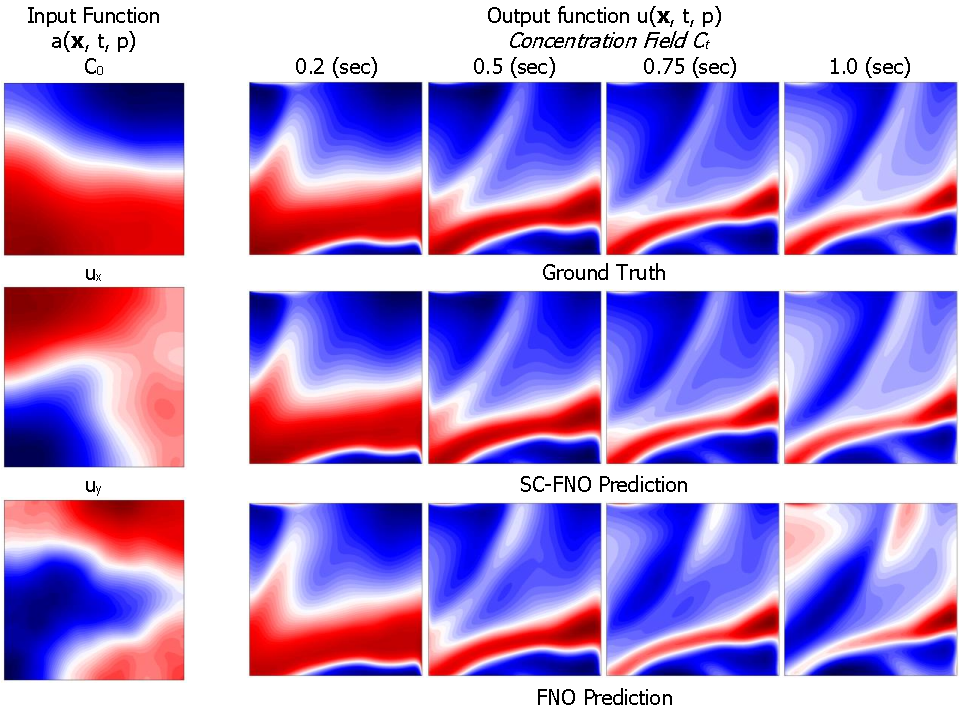
\includegraphics[width=0.8\textwidth, trim={0 0 0 0}, clip]{Figuers/PDE1_sample_prediction.pdf} % update filename if needed
%     \caption{\textbf{PDE1 Sample Prediction.}  
%     Representative forward prediction for PDE1 showing ground truth, SC-FNO, and FNO at selected time snapshots.  
%     SC-FNO remains closely aligned with the ground truth and avoids the dissipative errors observed in FNO.}
%     \label{fig:PDE1_sample_pred}
% \end{figure}




% Table for performances of models for inverse prediction of PDE1 without STD
\begin{table}[ht!]
\centering
\caption{\scriptsize\textbf{Comparison of Error Metrics Across Models Trained with Different Sample Sizes (Inverse)}}
\label{tab:pde1_inverse_nostd} 
\scriptsize
\setlength{\tabcolsep}{3pt}
\begin{tabular}{lcccccccc}
\hline
\textbf{Model} & \multicolumn{2}{c}{\textbf{1000 Samples}} & \multicolumn{2}{c}{\textbf{500 Samples}} & \multicolumn{2}{c}{\textbf{200 Samples}} & \multicolumn{2}{c}{\textbf{100 Samples}} \\
 & \textbf{Rel. \(L^2\)} & \textbf{MAE} & \textbf{Rel. \(L^2\)} & \textbf{MAE} & \textbf{Rel. \(L^2\)} & \textbf{MAE} & \textbf{Rel. \(L^2\)} & \textbf{MAE} \\
\hline
FNO & \(1.3 \times 10^{-1}\) & \(6.2 \times 10^{-2}\) & \(2.1 \times 10^{-1}\) & \(1.0 \times 10^{-1}\) & \(3.2 \times 10^{-1}\) & \(1.5 \times 10^{-1}\) & \(5.1 \times 10^{-1}\) & \(2.4 \times 10^{-1}\) \\
WNO & \(1.6 \times 10^{-1}\) & \(7.4 \times 10^{-2}\) & \(2.5 \times 10^{-1}\) & \(1.2 \times 10^{-1}\) & \(3.8 \times 10^{-1}\) & \(1.8 \times 10^{-1}\) & \(6.1 \times 10^{-1}\) & \(2.8 \times 10^{-1}\) \\
DeepONet & \(1.6 \times 10^{-1}\) & \(7.6 \times 10^{-2}\) & \(2.6 \times 10^{-1}\) & \(1.2 \times 10^{-1}\) & \(3.9 \times 10^{-1}\) & \(1.8 \times 10^{-1}\) & \(6.3 \times 10^{-1}\) & \(2.9 \times 10^{-1}\) \\
SC-FNO & \(\mathbf{1.3 \times 10^{-2}}\) & \(\mathbf{6.2 \times 10^{-3}}\) & \(\mathbf{1.5 \times 10^{-2}}\) & \(\mathbf{7.1 \times 10^{-3}}\) & \(\mathbf{1.8 \times 10^{-2}}\) & \(\mathbf{8.2 \times 10^{-3}}\) & \(\mathbf{2.1 \times 10^{-2}}\) & \(\mathbf{1.0 \times 10^{-2}}\) \\
SC-WNO & \(1.5 \times 10^{-2}\) & \(6.9 \times 10^{-3}\) & \(1.7 \times 10^{-2}\) & \(8.0 \times 10^{-3}\) & \(2.0 \times 10^{-2}\) & \(9.2 \times 10^{-3}\) & \(2.4 \times 10^{-2}\) & \(1.1 \times 10^{-2}\) \\
SC-DeepONet & \(1.8 \times 10^{-2}\) & \(8.4 \times 10^{-3}\) & \(2.1 \times 10^{-2}\) & \(9.7 \times 10^{-3}\) & \(2.4 \times 10^{-2}\) & \(1.1 \times 10^{-2}\) & \(2.9 \times 10^{-2}\) & \(1.4 \times 10^{-2}\) \\
\hline
\end{tabular}
\end{table}






% \begin{figure}[ht!]
%     \centering
%     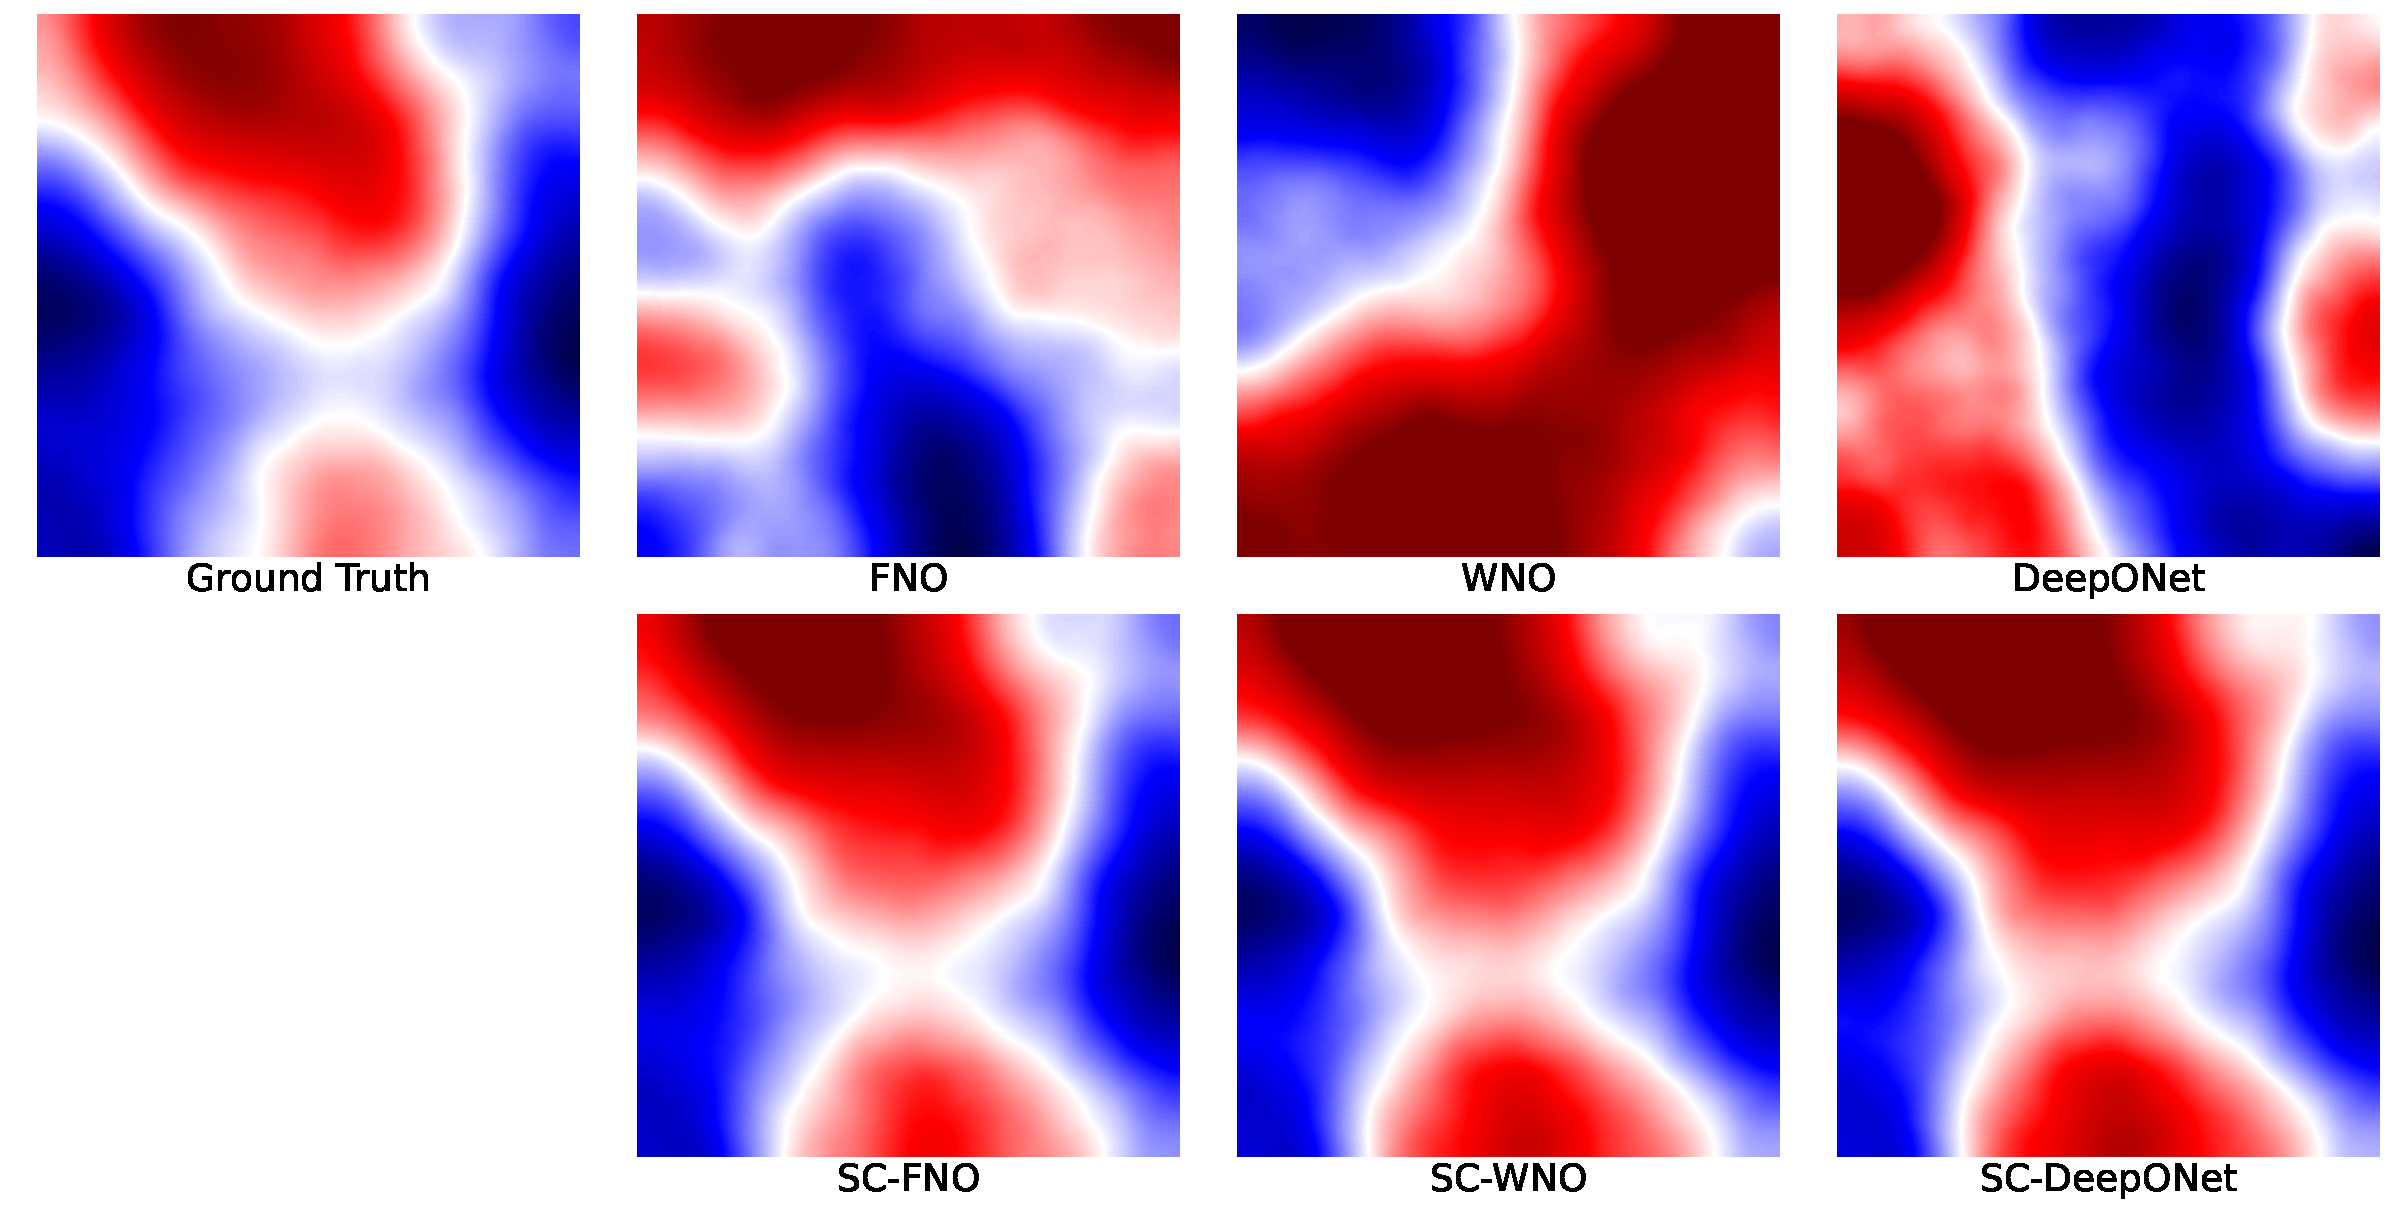
\includegraphics[width=0.8\textwidth]{Figuers/C0_ADE_reconstruction_clean_sample_10.pdf}
%     \caption{\textbf{Inversion of the initial concentration field for PDE1 (all models trained using 1000 samples).} 
%     Comparison of the true initial concentration field $C_0$ (top-left) with the inferred fields produced by FNO, WNO, DeepONet, and their sensitivity-constrained counterparts (SC-FNO, SC-WNO, SC-DeepONet).}    \label{fig:PDE1_C0_inversion}
%     \end{figure}


\begin{figure}[ht!]
    \centering
    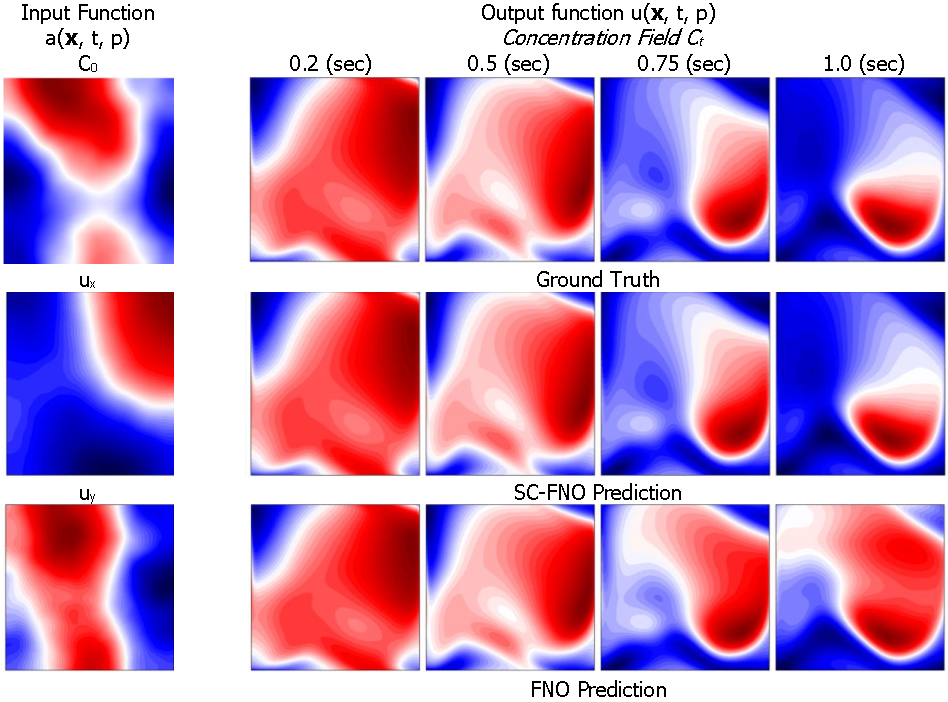
\includegraphics[width=0.8\textwidth, trim={0 0 0 0}, clip]{Figuers/PDE1_sample_prediction_1000_samples.pdf} % update filename if needed
    \caption{\scriptsize\textbf{PDE1 Sample Prediction.}  
    Representative forward prediction for PDE1 showing ground truth, SC-FNO, and FNO, trained on 1000 samples, at selected time snapshots.  
    SC-FNO remains closely aligned with the ground truth and avoids the dissipative errors observed in FNO.}
    \label{fig:PDE1_sample_pred}
\end{figure}






\begin{figure}[ht!]
    \centering
    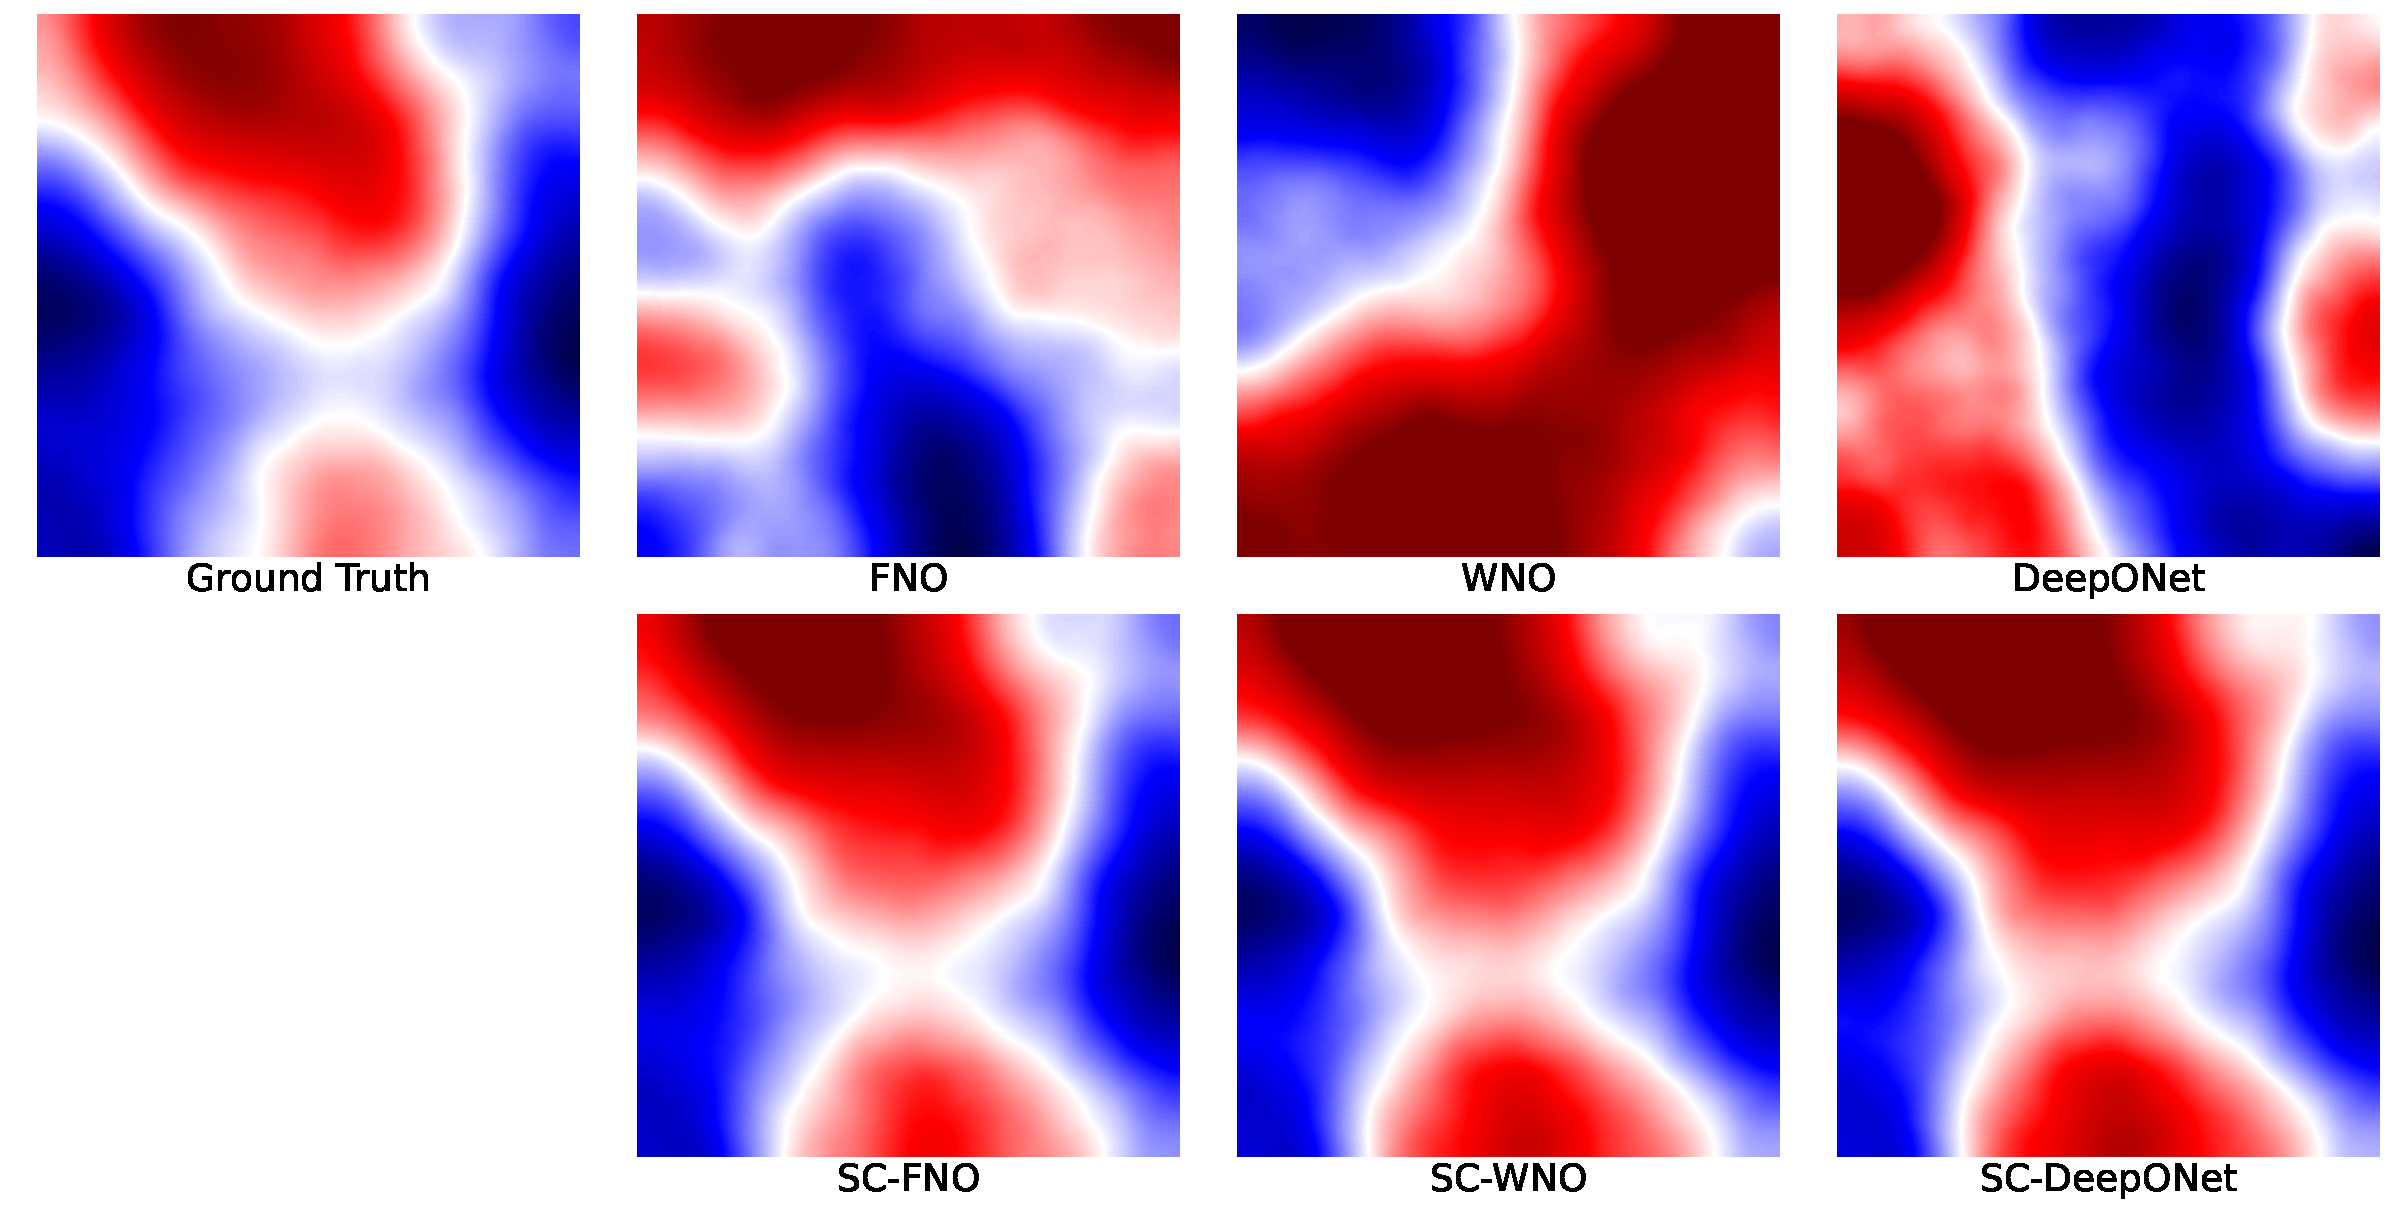
\includegraphics[width=0.8\textwidth]{Figuers/C0_ADE_reconstruction_clean_sample_10.pdf}
    \caption{\scriptsize\textbf{Inversion of the initial concentration field for PDE1 (all models trained using 200 samples).} 
    Comparison of the true initial concentration field $C_0$ (top-left) with the inferred fields produced by FNO, WNO, DeepONet, and their sensitivity-constrained counterparts (SC-FNO, SC-WNO, SC-DeepONet).}    \label{fig:PDE1_C0_inversion}
    \end{figure}



% % \clearpage
% % \section{PDE2: Navier--Stokes Equations with Spalart--Allmaras Closure}
\label{sec:NSE-SA}

\renewcommand{\thefigure}{D.\arabic{figure}}  % Number figures as A.1, A.2, ...
\renewcommand{\thetable}{D.\arabic{table}}  % Number tables as A.1, A.2, ...


\subsection*{Problem setup}
We simulate two-dimensional incompressible flows in the unit square domain \( \mathcal{X} = [0, 1] \times [0, 1] \) over the time interval \( t \in [0, T] \) with \( T = 25 \). The governing equations are expressed in vorticity--stream function form, coupled with the one-equation Spalart--Allmaras (S-A) turbulence model. Let \( \mathbf{x} = (x_1, x_2) \in \mathcal{X} \). The system reads:
\begin{align}
\nabla^2 \Psi &= -\Omega, \label{eq:streamfunction} \\[4pt]
\frac{\partial \Omega}{\partial t}
+ \frac{\partial \Psi}{\partial x_2} \frac{\partial \Omega}{\partial x_1}
- \frac{\partial \Psi}{\partial x_1} \frac{\partial \Omega}{\partial x_2}
&= \nabla \cdot \bigl[ (\nu + \nu_t) \nabla \Omega \bigr] + f(\mathbf{x}; \alpha, \beta), \label{eq:vorticity} \\[6pt]
\frac{\partial \tilde{\nu}}{\partial t}
+ \frac{\partial \Psi}{\partial x_2} \frac{\partial \tilde{\nu}}{\partial x_1}
- \frac{\partial \Psi}{\partial x_1} \frac{\partial \tilde{\nu}}{\partial x_2}
&= c_{b1} \tilde{S} \tilde{\nu}
+ \frac{1}{\sigma} \left[ \nabla \cdot \bigl( (\nu + \tilde{\nu}) \nabla \tilde{\nu} \bigr) + c_{b2} (\nabla \tilde{\nu})^2 \right]
- c_{w1} f_w \left( \frac{\tilde{\nu}}{d} \right)^2, \label{eq:SA}
\end{align}
where $\Psi$ denotes the stream function, $\Omega$ the vorticity, and the molecular viscosity is taken as $\nu \in [0.001,\,0.002]$, which corresponds to Reynolds numbers in the range $500$--$1000$. The turbulent eddy viscosity is modeled as $\nu_t = \tilde{\nu}\, f_{v1}$.
\[
f_{v1} = \frac{\chi^3}{\chi^3 + c_{v1}^3}, \quad \chi = \frac{\tilde{\nu}}{\nu}.
\]
The term \( f(\mathbf{x}; \alpha, \beta) \) is a parametric body force, and \( d \) is the distance to the nearest wall.

Physical boundary conditions are no-slip walls (\( \mathbf{u} = 0 \)), implying \( \Psi = 0 \) and \( \partial \Psi / \partial n = 0 \) on \( \partial \mathcal{X} \). Vorticity vanishes on walls via the initial mask \( m(x_1, x_2) = \sin(\pi x_1) \sin(\pi x_2) \).

The numerical solver uses zero wall boundary conditions in both directions for its finite difference discretization and fast Poisson solving. Physical wall conditions are enforced weakly through:
\begin{itemize}
    \item Initial vorticity masking to ensure \( \Omega_0 = 0 \) on wall-adjacent cells,
    \item Spectral projection of \( \Psi \) after each Poisson solve to satisfy \( \Psi = 0 \) on \( \partial \mathcal{X} \),
    \item Thom’s formula at each time step to enforce \( \mathbf{u} = 0 \) on walls.
\end{itemize}

The forward simulation uses a uniform fine grid of resolution \( 64 \times 64 \). The initial modified eddy viscosity is sampled from a Gaussian random field (GRF):
\[
\tilde{\nu}_0(\mathbf{x}) \sim \text{GRF}\bigl(p_{\min} = -2.5 \times 10^{-4},\; p_{\max} = 2.5 \times 10^{-4},\; \sigma = 1,\; \mathcal{X}\bigr).
\]

The initial vorticity \( \Omega_0 \) is generated on a coarse grid of resolution \( N_c \times N_c \), where \( N_c = 2^n \) and \( n \in \{2, 3, 4, 5, 6\} \) (corresponding to \( N_c \times N_c \in \{4\times4, 8\times8, 16\times16, 32\times32, 64\times64\} \)). For a given \( n \), the coarse field is
\[
\Omega_0^c(\mathbf{x}) = m(x_1, x_2) \cdot \text{GRF}\bigl(p_{\min} = -2.5,\; p_{\max} = 2.5,\; \sigma = 2,\; \mathcal{X}_c^n\bigr),
\]
upsampled to \( 64 \times 64 \) via pixel-wise repetition by factor \( 2^{6-n} \). This ensures zero vorticity on wall-adjacent fine-grid cells and introduces multiscale initial perturbations.

The forcing is
\[
f(\mathbf{x}; \alpha, \beta) = 0.1 \left[ \sin\!\bigl(\alpha (x_1 + x_2)\bigr) + \cos\!\bigl(\beta (x_1 + x_2)\bigr) \right],
\]
with \( \alpha, \beta \in [0, 3\pi] \) sampled uniformly.

\subsection*{Numerical Solver for the Turbulent Navier--Stokes Equations}

The system is recast as an ODE:
\[
\frac{d\mathbf{U}}{dt} = \text{RHS}(\mathbf{x}, t; p), \quad \mathbf{U} = [\Omega, \tilde{\nu}],
\]
with \( \Psi \) recovered via a fast Poisson solver (e.g., a Sine Transform) under zero wall computational boundary conditions. Spatial discretization uses second-order central finite differences on uniform grids. Time integration uses the Fourth Order Runge-Kutta solver from \texttt{torchdiffeq}, storing solutions at \( \Delta t = 0.1 \) over \( [0, 25.0] \), yielding \( n_t = 250 \) snapshots. The solver is fully differentiable, enabling adjoint-based gradients with respect to \( \Omega_0 \) and the forcing term.





\subsection*{Neural Operator Learning for the Turbulent Navier--Stokes Equations}

We employ neural operator learning to tackle the turbulent Navier--Stokes equations with the Spalart--Allmaras model over a spatial domain $\mathcal{X}$ and time $t \in [0, 25.0]$, discretized into $n_t$ snapshots (here, $n_t=250$ at $\Delta t=0.1\,\mathrm{s}$). The parametric, spatially varying forcing $f(\mathbf{x}; \alpha,\beta)$ acts as the parameter field $p(\mathbf{x})$ within the input function $a(\mathbf{x}, t, p)\in\mathcal{U}$. The solution state is $u(\mathbf{x}, t, p) = [\Psi(\mathbf{x}, t),\, \Omega(\mathbf{x}, t),\, \tilde{\nu}(\mathbf{x}, t)]$.

\paragraph{(I) Sequential multi-step forecasting (context $\rightarrow$ full-horizon prediction).}
We train a neural operator $\mathcal{G}_\theta$ within the SC-NO framework that consumes a short context of the trajectory together with the forcing field and predicts the remainder of the sequence in one shot. Concretely, the input consists of the initial segment of the solution field \( u(\mathbf{x}, t, p) \) over \( t \in [0, t_u] \) and the parameter field \( p(\mathbf{x}) = f(\mathbf{x}; \alpha, \beta) \):
\[
\mathcal{G}_\theta:\; \big(u(\mathbf{x}, t, p)\big)_{t \in [0, t_u]},\, p(\mathbf{x})\;\longrightarrow\; u(\mathbf{x}, t, p),
\quad (\mathbf{x}, t) \in \mathcal{X} \times [t_u,\,25.0].
\]
The training loss aggregates the state error over all predicted times together with a sensitivity regularizer. This regime corresponds to the “sequential prediction” setting used in the main text.



Additionally, to evaluate the model’s sensitivity to spatial resolution, we construct a family of simulations with multiresolution initial vorticity fields. Specifically, the base vorticity field \( \Omega_0^c(\mathbf{x}) \) is generated on coarse grids \( \mathcal{X}_c^n \) with \( N_c = 2^n \), \( n \in \{2,3,4,5,6\} \), and then upsampled to the working grid \( \mathcal{X} \) for training. Each resolution level thus defines a distinct realization of the input sequence \( \big(u(\mathbf{x}, t, p)\big)_{t \in [0, t_u]} \), differing only in the spatial smoothness and detail of the initial vorticity \( \Omega_0(\mathbf{x}) \). The operator learns the mapping  
\[
\mathcal{G}_\theta:\; \big(u(\mathbf{x}, t, p)\big)_{t \in [0, t_u]},\, p(\mathbf{x})\;\longrightarrow\; u(\mathbf{x}, t, p),
\quad (\mathbf{x}, t) \in \mathcal{X} \times [t_u,\,25.0],
\]
allowing us to systematically assess how prediction accuracy and learned sensitivities vary across different resolutions of the initial vorticity field.




\paragraph{(II) One-step transition with autoregressive rollout (rollout model).}  
In this regime, we train a \emph{transition operator} that advances the state by a single time step given the current state and the forcing field. During training, the operator is supervised on consecutive snapshot pairs using teacher forcing. Specifically, it learns the mapping
\[
\mathcal{F}_\theta:\; \big(u(\cdot,t,p),\, p(\mathbf{x})\big)\;\longrightarrow\; u(\cdot,t+\Delta t,p),
\]
with training pairs $\big(u(\cdot,t,p),\, u(\cdot,t+\Delta t,p)\big)$ drawn from the first 125 snapshots, corresponding to $t \in [0,12.5]$\,s. To improve robustness, the predicted states used during training are perturbed with controlled noise before being fed back as inputs, preventing the model from overfitting to perfectly clean trajectories.  

At inference time, the learned operator is applied recursively in an autoregressive manner to generate full trajectories. Starting from the initial condition $u(\cdot,0,p)$, we roll the model forward for 250 steps to cover the entire horizon $[0,25.0]$\,s:  
\[
\hat{u}(\cdot,t+\Delta t,p)=\mathcal{F}_\theta\!\big(\hat{u}(\cdot,t,p),\,p\big), \quad t=0,\Delta t,2\Delta t,\ldots,25.0-\Delta t.
\]
This formulation explicitly probes long-horizon stability and error accumulation: the model is trained only on short-range one-step transitions ($0$–$12.5$\,s) but evaluated on the full $0$–$25$\,s trajectory (250 snapshots).  

\subsection*{Adjoint-Based Sensitivity Computation for the Turbulent Navier--Stokes Equations}
\label{sec:adjoint_nse}

To compute sensitivities of the final-time vorticity field $\Omega(\mathbf{x}, T)$ with respect to the initial vorticity $\Omega_0(\mathbf{x})$ and the forcing $f(\mathbf{x}, t; \alpha, \beta)$, we derive the continuous adjoint system. The adjoint method is a powerful technique for efficiently computing the sensitivity of a scalar objective functional, $J$, to a large number of input parameters or fields (such as initial conditions $\Omega_0$ or forcing $f$). Its primary advantage is that the computational cost of obtaining the gradient is \textbf{independent} of the number of input parameters. The method relies on constructing a Lagrangian, $\mathcal{L}$, which augments the objective functional with the governing PDEs, enforced as constraints via Lagrange multipliers (the adjoint variables, e.g., $\lambda_\Omega, \lambda_{\tilde{\nu}}$). By requiring the first variation of the Lagrangian ($\delta\mathcal{L}$) to be zero with respect to the state variables, a new set of linear PDEs—the \textbf{adjoint equations}—is derived.

These adjoint equations are solved \textbf{backward in time}, starting from a terminal condition derived from the objective functional at $t=T$. The resulting adjoint field, $\lambda(\mathbf{x}, 0)$, at the initial time $t=0$ (or integrated over time for forcing) provides the exact functional derivative (gradient) of $J$ with respect to the parameters. This allows the gradient for all parameters to be computed from just one forward solve of the primal equations and one backward solve of the adjoint equations.

\subsubsection*{Cost Functional}

The cost functional is the integrated final vorticity:
\begin{equation}
J = \int_{\mathcal{X}} \Omega(\mathbf{x}, T) \, d\mathbf{x}.
\end{equation}

\subsubsection*{Lagrangian Formulation}

The Lagrangian is
\begin{align}
\mathcal{L} &= \int_{\mathcal{X}} \Omega(T) \, d\mathbf{x} \notag \\[4pt]
&\quad + \int_0^T \int_{\mathcal{X}} \lambda_{\Omega} \left[
\frac{\partial \Omega}{\partial t}
+ (\mathbf{u} \cdot \nabla) \Omega
- \nabla \cdot \bigl( \nu_{\text{eff}}(\tilde{\nu}) \nabla \Omega \bigr)
- f
\right] d\mathbf{x} \, dt \notag \\[4pt]
&\quad + \int_0^T \int_{\mathcal{X}} \lambda_{\tilde{\nu}} \left[
\frac{\partial \tilde{\nu}}{\partial t}
+ (\mathbf{u} \cdot \nabla) \tilde{\nu}
- \frac{1}{\sigma} \nabla \cdot \bigl( (\nu + \tilde{\nu}) \nabla \tilde{\nu} \bigr)
- \frac{c_{b2}}{\sigma} (\nabla \tilde{\nu})^2
- R(\Omega, \tilde{\nu})
\right] d\mathbf{x} \, dt \notag \\[4pt]
&\quad + \int_0^T \int_{\mathcal{X}} \lambda_{\Psi} \left[
\nabla^2 \Psi + \Omega
\right] d\mathbf{x} \, dt,
\end{align}
where $\mathbf{u} = \nabla^\perp \Psi$, $\nu_{\text{eff}}(\tilde{\nu}) = \nu + \tilde{\nu} f_{v1}(\tilde{\nu})$, and
\[
R(\Omega, \tilde{\nu}) = c_{b1} \tilde{S} \tilde{\nu} - c_{w1} f_w \left( \frac{\tilde{\nu}}{d} \right)^2.
\]

\subsubsection*{Adjoint Equations}

The first variation $\delta \mathcal{L} = 0$ with respect to $(\Psi, \Omega, \tilde{\nu})$ yields the adjoint system. Integration by parts in space and time is performed. Boundary terms are eliminated using primal wall conditions.

\textbf{Adjoint Poisson Equation} (from $\delta \Psi$):
\begin{equation}
\nabla^2 \lambda_{\Psi}
= -\nabla^\perp \cdot (\lambda_{\Omega} \nabla \Omega)
  -\nabla^\perp \cdot (\lambda_{\tilde{\nu}} \nabla \tilde{\nu}).
\end{equation}

\textbf{Adjoint Vorticity Equation} (from $\delta \Omega$):
\begin{equation}
-\frac{\partial \lambda_{\Omega}}{\partial t}
= \mathbf{u} \cdot \nabla \lambda_{\Omega}
  + \nabla \cdot \bigl( \nu_{\text{eff}} \nabla \lambda_{\Omega} \bigr)
  + \lambda_{\Psi}
  + \lambda_{\tilde{\nu}} \frac{\partial R}{\partial \Omega},
\end{equation}
with
\[
\frac{\partial R}{\partial \Omega}
= c_{b1} \tilde{\nu} \frac{\partial \tilde{S}}{\partial \Omega},
\qquad
\frac{\partial \tilde{S}}{\partial \Omega}
= \operatorname{sgn}(\Omega)
\quad \text{(regularized as $\tanh(k \Omega)$ in practice)}.
\]

\textbf{Adjoint Spalart--Allmaras Equation} (from $\delta \tilde{\nu}$):
\begin{equation}
-\frac{\partial \lambda_{\tilde{\nu}}}{\partial t}
= \mathbf{u} \cdot \nabla \lambda_{\tilde{\nu}}
  + \frac{1}{\sigma} \nabla \cdot \bigl( (\nu + \tilde{\nu}) \nabla \lambda_{\tilde{\nu}} \bigr)
  - \nabla \cdot \left( \frac{2 c_{b2}}{\sigma} \lambda_{\tilde{\nu}} \nabla \tilde{\nu} \right)
  + \lambda_{\tilde{\nu}} \frac{\partial R}{\partial \tilde{\nu}}
  - \frac{\partial \nu_{\text{eff}}}{\partial \tilde{\nu}} (\nabla \lambda_{\Omega} \cdot \nabla \Omega).
\end{equation}

\subsubsection*{Adjoint Terminal and Boundary Conditions}

\textbf{Terminal conditions} (at $t = T$):
\begin{align}
\lambda_{\Omega}(\mathbf{x}, T) &= -1, \\
\lambda_{\tilde{\nu}}(\mathbf{x}, T) &= 0.
\end{align}

\textbf{Boundary conditions} (on $\partial \mathcal{X}$, $0 \leq t < T$):
\begin{itemize}
    \item $\lambda_{\Psi} = 0$ \quad (from primal $\Psi = 0$),
    \item $\lambda_{\tilde{\nu}} = 0$ \quad (from primal $\tilde{\nu} = 0$),
    \item $\lambda_{\Omega} = 0$ \quad (from primal $\Omega = 0$: $\delta \Omega = 0$ on boundary $\implies$ adjoint inherits Dirichlet).
\end{itemize}

The adjoint system is solved backward in time from $t = T$ to $t = 0$.

\subsubsection*{Sensitivity with Respect to Initial Vorticity $\Omega_0$}

From the time-boundary term at $t=0$:
\begin{equation}
\boxed{
\frac{\delta J}{\delta \Omega_0}(\mathbf{x})
= -\lambda_{\Omega}(\mathbf{x}, 0)
}
\end{equation}

\subsubsection*{Sensitivity with Respect to Forcing Field $f$}

From the explicit $f$ term in the Lagrangian:
\begin{equation}
\boxed{
\frac{\delta J}{\delta f}(\mathbf{x}, t)
= -\lambda_{\Omega}(\mathbf{x}, t),
\qquad
\frac{\delta J}{\delta f}(\mathbf{x})
= -\int_0^T \lambda_{\Omega}(\mathbf{x}, t) \, dt
}
\end{equation}

These sensitivities are exact in the continuous setting and provide the full gradient of the final vorticity field with respect to initial conditions and forcing.

\subsubsection*{Degree of freedom (DOF) experiment}
Here, DOF refers to the number of independent values in the spatially varying input field (i.e., the intrinsic resolution of the input field, such as the initial vorticity $\omega_0$ for RANS). To isolate DOF as the sole varying factor, we fix the RANS solution grid at $64\times64$ and vary only the intrinsic resolution of the input field ($\omega_0$); each realization is upsampled to the common grid prior to training, with all other parameters held constant. For each DOF level ($4^2$, $16^2$, $64^2$), we train the models using four dataset sizes (100, 200, 500, and 1000 samples of different initial vorticity fields), record the total wall-clock compute time (data preparation + Jacobian calculation + training), and plot the resulting $L^2$ errors against these costs (Figure~\ref{fig:scaling_curve}a). Differences in total compute time primarily reflect the number of training samples required. Smooth curves are then fitted to the error--cost points for each method. Figure~\ref{fig:scaling_curve}b is obtained by intersecting these fitted curves with the horizontal line $L^2 = 0.075$. %, allowing us to read off the compute cost needed to reach that accuracy level at each DOF.

\subsection*{Additional results for PDE2}
% Table for performances of models for forward prediction of PDE2 without STD (rounded)
\begin{table}[ht!]
\centering
\caption{\textbf{Comparison of Error Metrics Across Models Trained with Different Sample Sizes (Forward)}}
\label{tab:pde2_forward_nostd}
\scriptsize
\setlength{\tabcolsep}{3pt}
\begin{tabular}{lcccccccc}
\hline
\textbf{Model} & \multicolumn{2}{c}{\textbf{1000 Samples}} & \multicolumn{2}{c}{\textbf{500 Samples}} & \multicolumn{2}{c}{\textbf{200 Samples}} & \multicolumn{2}{c}{\textbf{100 Samples}} \\
 & \textbf{Rel. \(L^2\)} & \textbf{MAE} & \textbf{Rel. \(L^2\)} & \textbf{MAE} & \textbf{Rel. \(L^2\)} & \textbf{MAE} & \textbf{Rel. \(L^2\)} & \textbf{MAE} \\
\hline
FNO        & \(6.9 \times 10^{-2}\) & \(6.8 \times 10^{-3}\) & \(1.9 \times 10^{-1}\) & \(1.8 \times 10^{-2}\) & \(5.7 \times 10^{-1}\) & \(5.4 \times 10^{-2}\) & \(1.3 \times 10^{0}\) & \(1.3 \times 10^{-1}\) \\
WNO        & \(7.5 \times 10^{-2}\) & \(7.3 \times 10^{-3}\) & \(2.0 \times 10^{-1}\) & \(2.0 \times 10^{-2}\) & \(6.0 \times 10^{-1}\) & \(5.8 \times 10^{-2}\) & \(1.4 \times 10^{0}\) & \(1.4 \times 10^{-1}\) \\
DeepONet   & \(8.1 \times 10^{-2}\) & \(7.9 \times 10^{-3}\) & \(2.2 \times 10^{-1}\) & \(2.1 \times 10^{-2}\) & \(6.6 \times 10^{-1}\) & \(6.3 \times 10^{-2}\) & \(1.5 \times 10^{0}\) & \(1.5 \times 10^{-1}\) \\
SC-FNO     & \(\mathbf{2.9 \times 10^{-2}}\)& \(\mathbf{2.2 \times 10^{-3}}\) & \(\mathbf{3.9 \times 10^{-2}}\) & \(\mathbf{7.4 \times 10^{-3}}\) & \(\mathbf{6.6 \times 10^{-2}}\) & \(\mathbf{1.3 \times 10^{-2}}\) & \(\mathbf{1.5 \times 10^{-1}}\) & \(\mathbf{3.0 \times 10^{-2}}\) \\
SC-WNO     & \(3.4\times 10^{-2}\)& \(2.3 \times 10^{-3}\) & \(3.9 \times 10^{-2}\) & \(7.6 \times 10^{-3}\) & \(6.8 \times 10^{-2}\) & \(1.3 \times 10^{-2}\) & \(1.7 \times 10^{-1}\) & \(3.1 \times 10^{-2}\) \\
SC-DeepONet& \(4.1 \times 10^{-2}\)& \(2.9 \times 10^{-3}\) & \(5.1 \times 10^{-2}\) & \(9.7 \times 10^{-3}\) & \(8.6 \times 10^{-2}\) & \(1.7 \times 10^{-2}\) & \(2.0 \times 10^{-1}\) & \(3.9 \times 10^{-2}\) \\
\hline
\end{tabular}
\end{table}




% \begin{figure}[ht!]
%     \centering
%     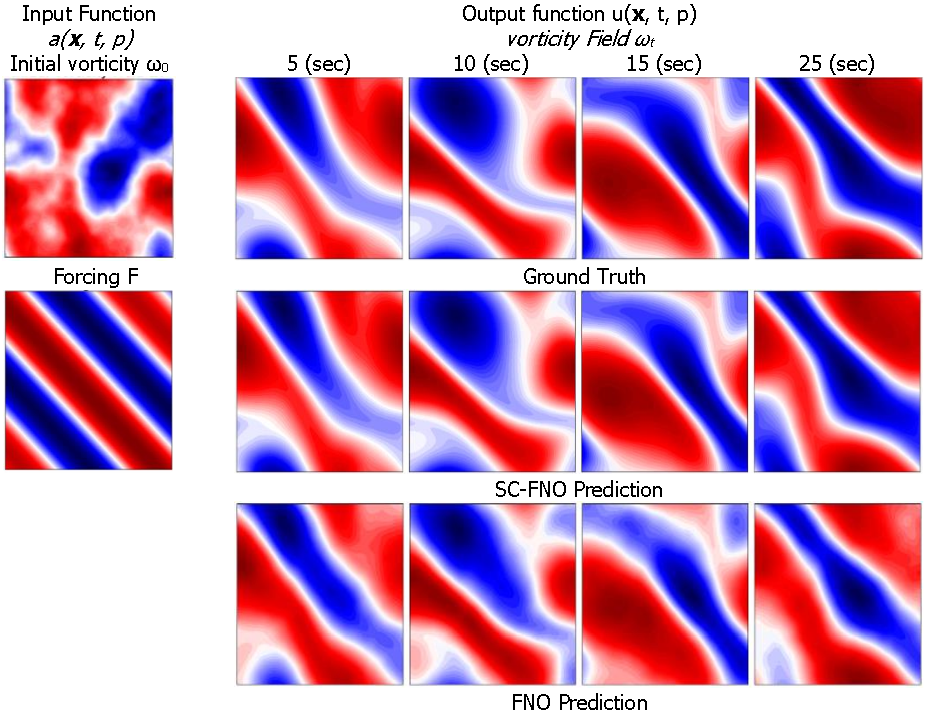
\includegraphics[width=0.8\textwidth, trim={0 0 0 0}, clip]{Figuers/PDE2_sample_prediction.pdf} % update filename if needed
%     \caption{\textbf{PDE2 Sample Prediction.}  
%     Representative forward prediction for PDE2 showing ground truth, SC-FNO, and FNO across selected time snapshots.  
%     SC-FNO maintains close agreement with the ground truth, while FNO exhibits dissipative drift and smeared structures over time.}
%     \label{fig:PDE2_sample_pred}
% \end{figure}



% Table for performances of models for inverse prediction of PDE2 without STD (rounded)
\begin{table}[ht!]
\centering
\caption{\scriptsize\textbf{Comparison of Error Metrics Across Models Trained with Different Sample Sizes (Inverse) PDE2}}
\label{tab:pde2_inverse_nostd}
\scriptsize
\setlength{\tabcolsep}{3pt}
\begin{tabular}{lcccccccc}
\hline
\textbf{Model} & \multicolumn{2}{c}{\textbf{1000 Samples}} & \multicolumn{2}{c}{\textbf{500 Samples}} & \multicolumn{2}{c}{\textbf{200 Samples}} & \multicolumn{2}{c}{\textbf{100 Samples}} \\
 & \textbf{Rel. \(L^2\)} & \textbf{MAE} & \textbf{Rel. \(L^2\)} & \textbf{MAE} & \textbf{Rel. \(L^2\)} & \textbf{MAE} & \textbf{Rel. \(L^2\)} & \textbf{MAE} \\
\hline
FNO        & \(4.7 \times 10^{-1}\) & \(5.0 \times 10^{-2}\) & \(6.7 \times 10^{-1}\) & \(7.2 \times 10^{-2}\) & \(9.6 \times 10^{-1}\) & \(1.0 \times 10^{-1}\) & \(1.4 \times 10^{0}\) & \(1.4 \times 10^{-1}\) \\
WNO        & \(5.6 \times 10^{-1}\) & \(5.9 \times 10^{-2}\) & \(7.9 \times 10^{-1}\) & \(8.4 \times 10^{-2}\) & \(1.1 \times 10^{0}\) & \(1.2 \times 10^{-1}\) & \(1.6 \times 10^{0}\) & \(1.7 \times 10^{-1}\) \\
DeepONet   & \(5.8 \times 10^{-1}\) & \(6.1 \times 10^{-2}\) & \(8.0 \times 10^{-1}\) & \(8.7 \times 10^{-2}\) & \(1.2 \times 10^{0}\) & \(1.2 \times 10^{-1}\) & \(1.6 \times 10^{0}\) & \(1.7 \times 10^{-1}\) \\
SC-FNO     & \(\mathbf{6.1 \times 10^{-2}}\) & \(\mathbf{5.2 \times 10^{-3}}\) & \(\mathbf{6.8 \times 10^{-2}}\) & \(\mathbf{5.8 \times 10^{-3}}\) & \(\mathbf{8.0 \times 10^{-2}}\) & \(\mathbf{6.8 \times 10^{-3}}\) & \(\mathbf{9.6 \times 10^{-2}}\) & \(\mathbf{8.2 \times 10^{-3}}\) \\
SC-WNO     & \(6.8 \times 10^{-2}\) & \(5.8 \times 10^{-3}\) & \(7.6 \times 10^{-2}\) & \(6.5 \times 10^{-3}\) & \(9.0 \times 10^{-2}\) & \(7.6 \times 10^{-3}\) & \(1.1 \times 10^{-1}\) & \(9.2 \times 10^{-3}\) \\
SC-DeepONet& \(8.3 \times 10^{-2}\) & \(7.0 \times 10^{-3}\) & \(9.3 \times 10^{-2}\) & \(7.9 \times 10^{-3}\) & \(1.1 \times 10^{-1}\) & \(9.3 \times 10^{-3}\) & \(1.3 \times 10^{-1}\) & \(1.1 \times 10^{-2}\) \\
\hline
\end{tabular}
\end{table}






% \begin{figure}[ht!]
%     \centering
%     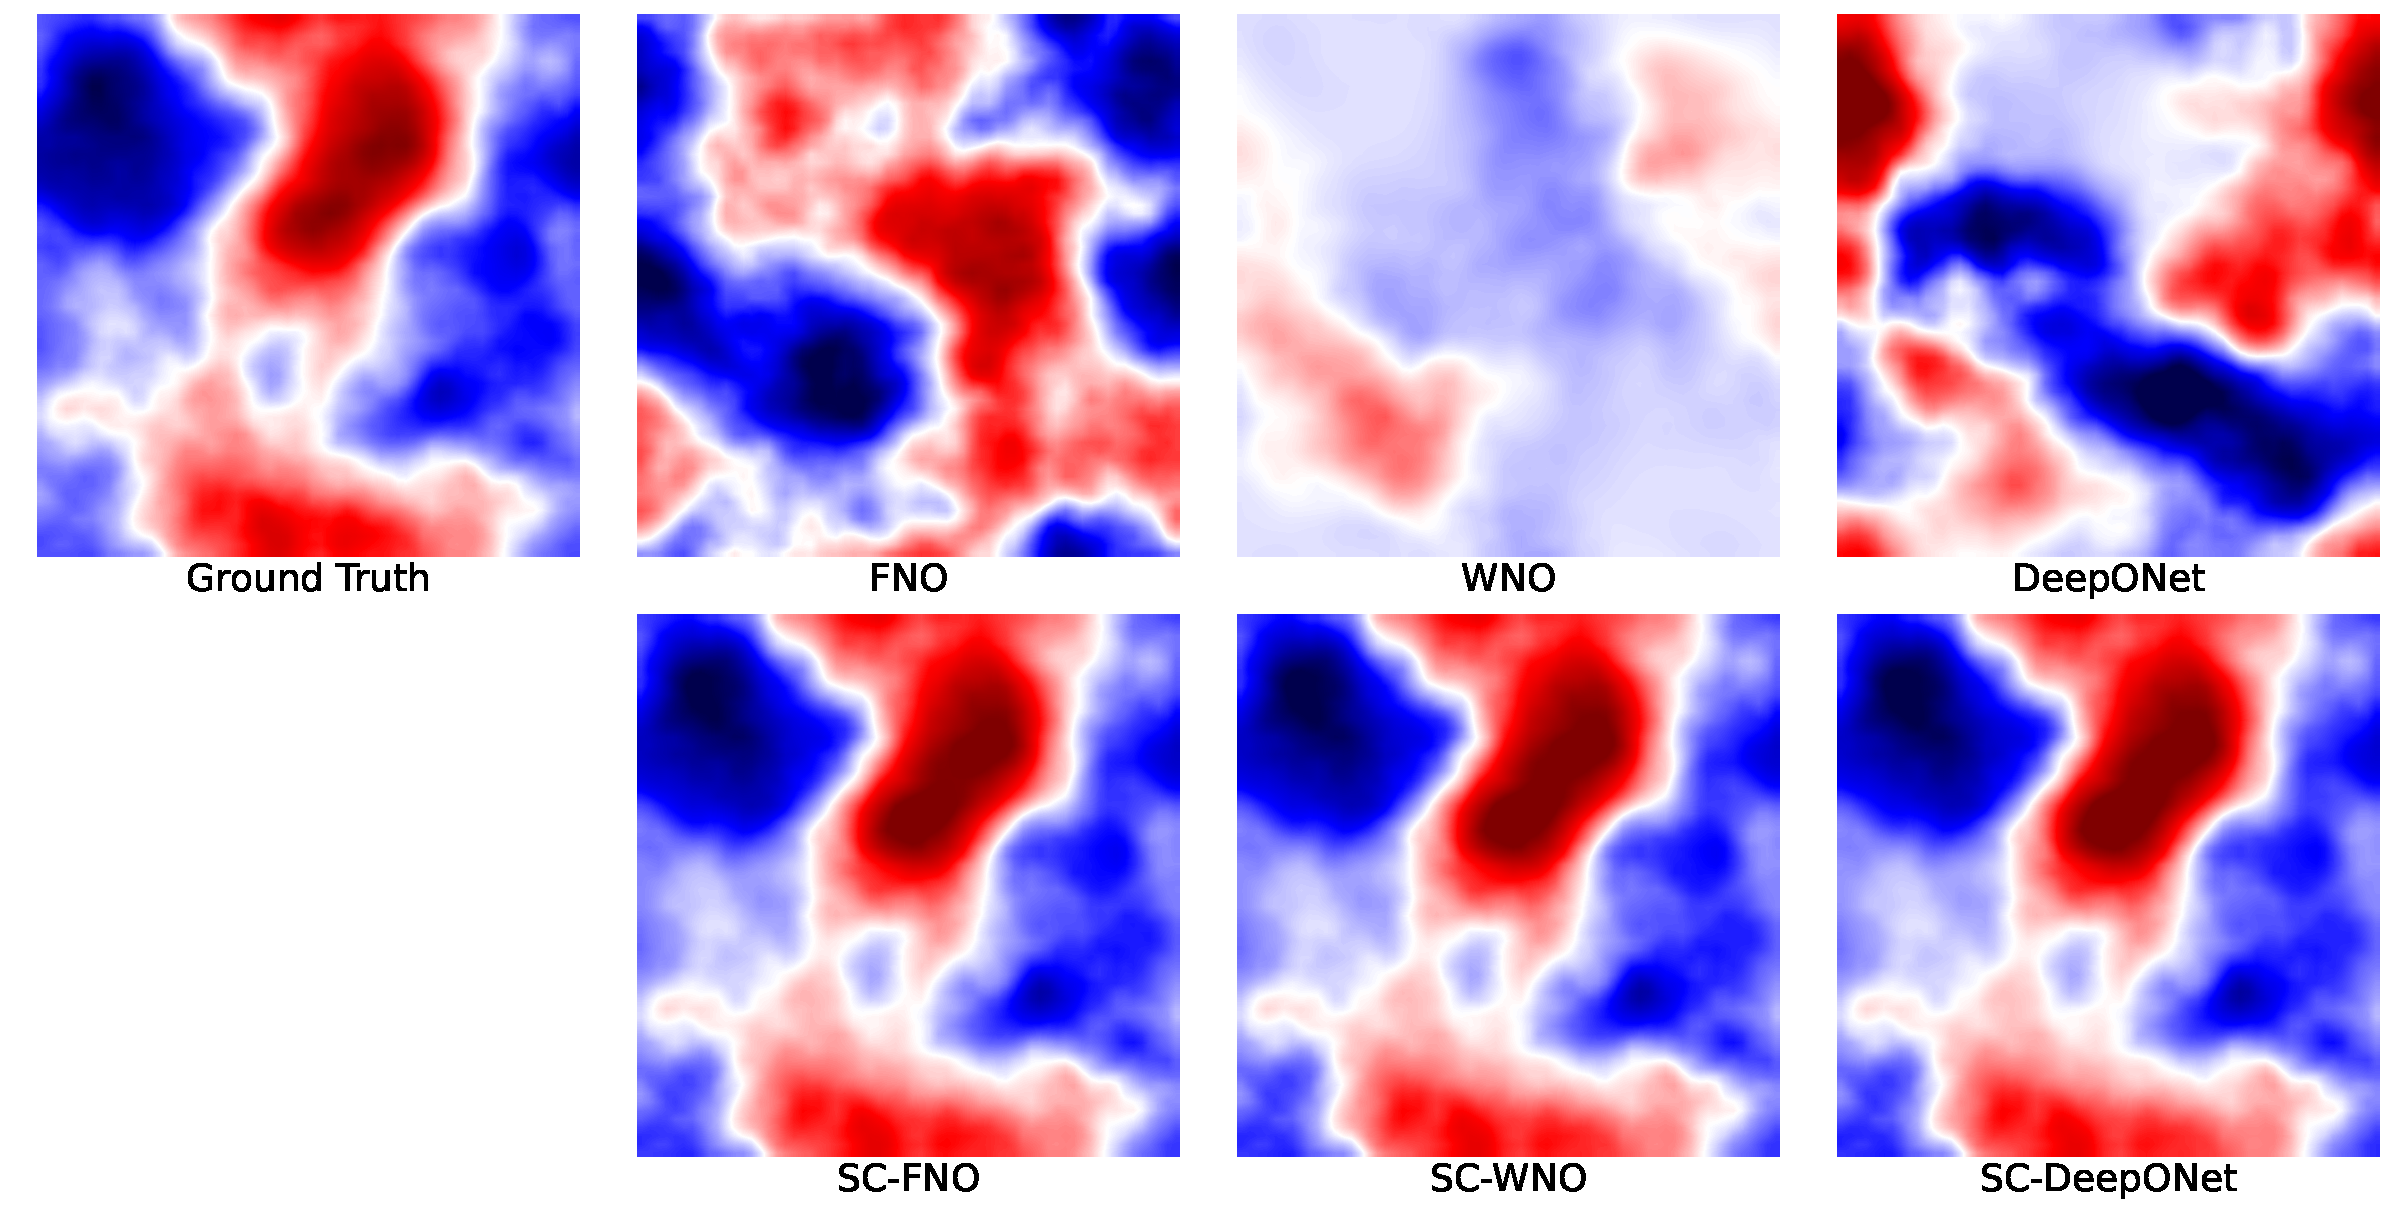
\includegraphics[width=0.8\textwidth]{Figuers/vorticity_reconstruction_clean_sample_5.pdf}
%     \caption{\textbf{Inversion of the Initial Vorticity Field for PDE2 (all models trained using 1000 samples).}
%     Comparison of the true initial vorticity field $\omega_0$ (top-left) with the inferred fields produced by FNO, WNO, DeepONet, and their sensitivity-constrained counterparts (SC-FNO, SC-WNO, SC-DeepONet). 
%     }
%     \label{fig:PDE2_w0_inversion}
% \end{figure}



\begin{figure}[ht!]
    \centering
    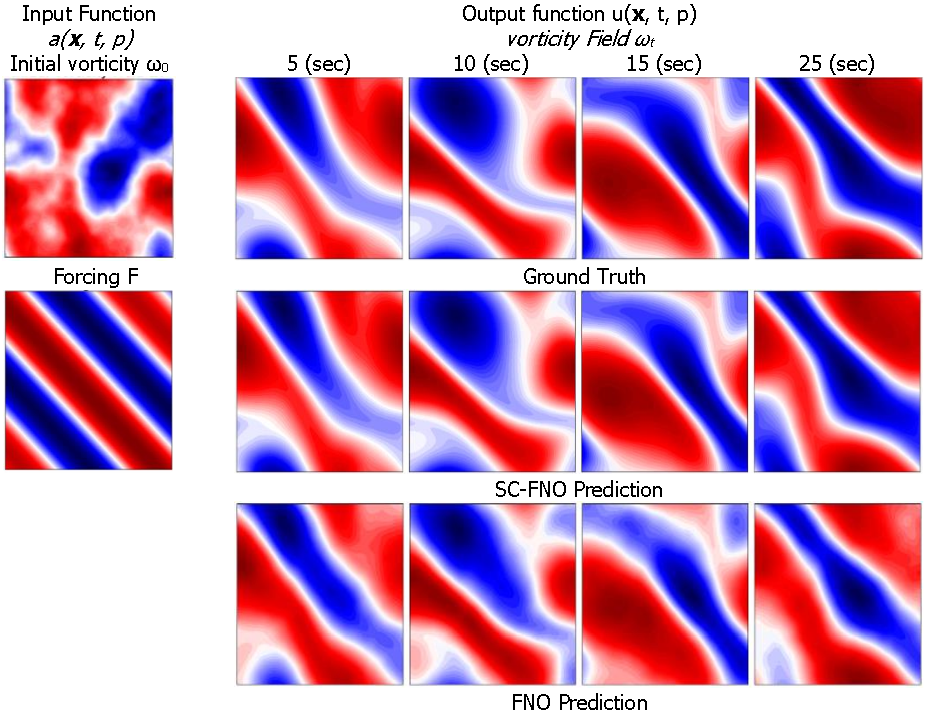
\includegraphics[width=0.8\textwidth, trim={0 0 0 0}, clip]{Figuers/PDE2_sample_prediction.pdf} % update filename if needed
    \caption{\scriptsize\textbf{PDE2 Sample Prediction.}  
    Representative forward predictions for PDE2 comparing the ground truth, SC-FNO, and FNO, trained on 200 samples, at selected time snapshots. SC-FNO maintains close agreement with the ground truth, while FNO exhibits dissipative drift and progressively smeared structures over time.}
    \label{fig:PDE2_sample_pred}
\end{figure}


\begin{figure}[ht!]
    \centering
    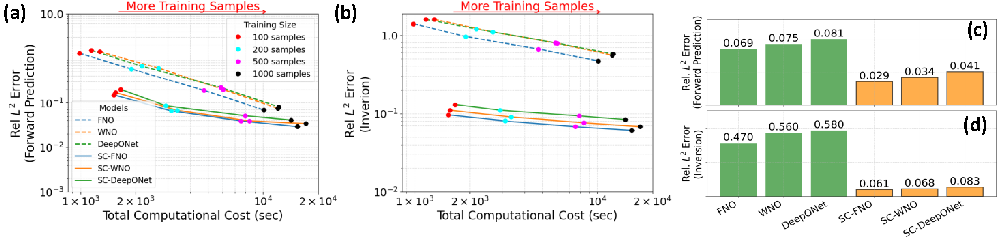
\includegraphics[width=0.98\textwidth, trim={0 0 0 0}, clip]{Figuers/PDE2_summeries.pdf}
    \caption{\scriptsize\textbf{Accuracy–computation trade-off for
    Turbulent Navier--Stokes with Spalart--Allmaras model (PDE2).}
    Sensitivity constraints achieve substantially lower errors for the same
    computational budget as training samples increase.
    (a) Relative $L^2$ error for forward prediction versus total computation time.
    (b) Relative $L^2$ error for inversion (reconstruction of $\omega$) versus total computation time.
    (c) Relative $L^2$ error for forward prediction at 1000 training samples.
    (d) Relative $L^2$ error for inversion at 1000 training samples.}
    \label{fig:PDE2_summerised}   
    \end{figure}



\begin{figure}[ht!]
    \centering
    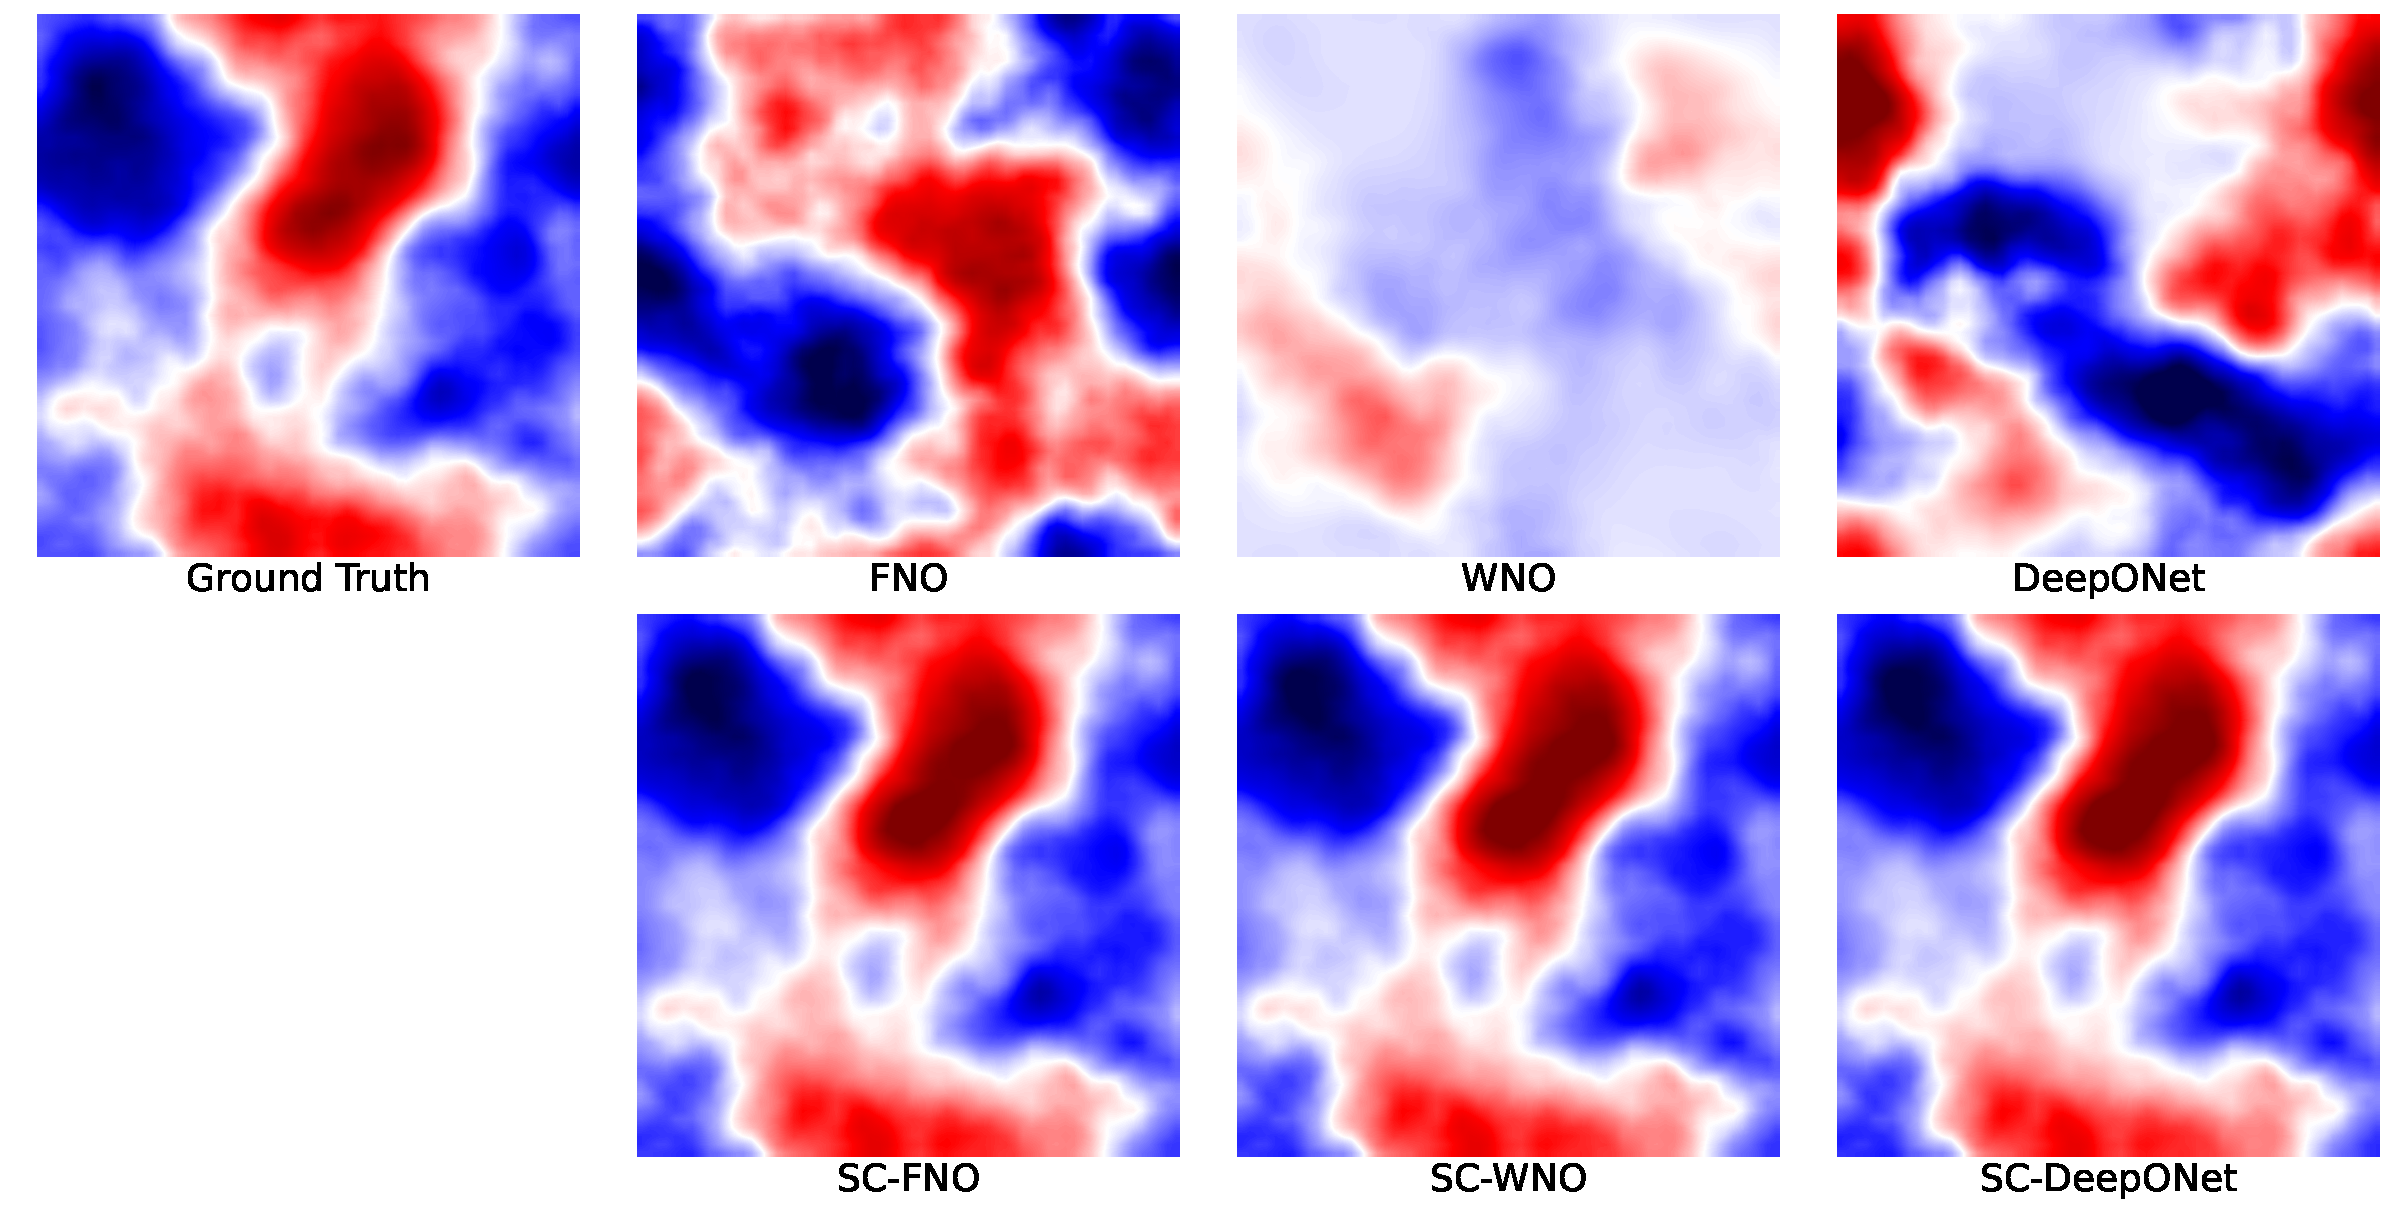
\includegraphics[width=0.8\textwidth]{Figuers/vorticity_reconstruction_clean_sample_5.pdf}
    \caption{\scriptsize\textbf{Inversion of the Initial Vorticity Field for PDE2 (all models trained using 200 samples).}
    Comparison of the true initial vorticity field $\omega_0$ (top-left) with the inferred fields produced by FNO, WNO, DeepONet, and their sensitivity-constrained counterparts (SC-FNO, SC-WNO, SC-DeepONet). 
    }
    \label{fig:PDE2_w0_inversion}
\end{figure}


% % \clearpage
% % \section{PDE3: 2D Shallow Water Equations for the Tohoku 2011 Tsunami}
\label{sec:SWE-Tohoku}

\renewcommand{\thefigure}{E.\arabic{figure}}  % Number figures as A.1, A.2, ...
\renewcommand{\thetable}{E.\arabic{table}}  % Number tables as A.1, A.2, ...


\subsection*{Overview}
We evaluate the feasibility of near-real-time large-scale tsunami inversion and forecasting using SC-NOs, governed by the hyperbolic Shallow Water equations, based on the 2011 Tohoku event. Variability arises from earthquake-induced seafloor deformation computed using the Okada model \citep{grilli2013numerical} with different geometries and epicenter locations. We use noise-contaminated synthetic water-level observations at sea-buoy locations from the first 30 minutes as observations for the inverse source identification, followed by forward forecasting. The inversion first estimates an initial guess of the seafloor deformation field, restricts it to the Okada representation, and then optimizes the Okada model parameters via the pretrained neural operators (Methods). All neural operators (FNO and SC-FNO) are pretrained on high-resolution simulations from a observationally-validated finite-volume solver (Supplementary Figure~\ref{fig:tohoku_validation}), coarsened to the NO grid resolutions. They receive deformation fields $\Delta z_b(\mathbf{x})$ and an initial water stage ($t_u = 1$) as inputs and predict the remaining $t_G = 50$ time steps. We calculate the sensitivity (Jacobian) of the final water stage with respect to bed topography using adjoint-sensitivity analysis.


\subsection*{Problem setup}
We solve the shallow water equations (SWE) with Manning friction over a two-dimensional ocean domain \( \mathcal{X} = [0, L] \times [0, L] \) and time \( t \in [0, T] \). This formulation captures wave propagation, coastal inundation, and wet-dry dynamics. Given spatial coordinates \(\textbf{x} = (x, y) \in \mathcal{X} \), the governing SWE system is:



\begin{equation}
\frac{\partial}{\partial t}
\begin{pmatrix}
h \\[3pt]
m_x \\[3pt]
m_y
\end{pmatrix}
+ \nabla \cdot
\begin{pmatrix}
h \mathbf{u} \\[5pt]
h u \mathbf{u} + \tfrac{1}{2}\,g\,h^2 \,\mathbf{I}_x \\[3pt]
h v \mathbf{u} + \tfrac{1}{2}\,g\,h^2 \,\mathbf{I}_y
\end{pmatrix}
=
\begin{pmatrix}
0 \\[4pt]
-\,g\,h\,\frac{\partial z_b}{\partial x} \;-\; \bigl(\text{friction}_x\bigr) \\[6pt]
-\,g\,h\,\frac{\partial z_b}{\partial y} \;-\; \bigl(\text{friction}_y\bigr)
\end{pmatrix}.
\end{equation}

Here, \( h \) is the water depth, \( \mathbf{m} = (m_x, m_y) = (h u, h v) \) is the depth-integrated momentum, \( \mathbf{u} = (u, v) \) is the velocity, and \( z_b(x, y) \) represents the bed elevation. The source terms include the bed slope and Manning friction:

\begin{equation}
\text{friction}_x = g n^2 \|\mathbf{u}\| \frac{h u}{h^{7/3}}, 
\quad
\text{friction}_y = g n^2 \|\mathbf{u}\| \frac{h v}{h^{7/3}}.
\end{equation}
To represent wet-dry dynamics, dry regions are modeled by setting \( h = 0 \) when the water depth falls below a threshold. no reflection boundary conditions are imposed in both \( x \) and \( y \) directions to simulate an open ocean. 

\subsection*{Modeling Seafloor Deformation Using the Okada Dislocation Model}
The Tohoku 2011 tsunami was triggered by an Mw 9.0 earthquake along the Japan Trench on March 11, 2011. To simulate this event, we investigate a 1000 km × 1000 km region as illustrated in Figure \ref{fig:bed_elevation}, using real bathymetry data to define the pre-earthquake seabed topography \( z_{b0}(\textbf{x}) \). This dataset, obtained from ETOPO 2022 at 30 Arc-Second resolution, provides an accurate baseline representation of the ocean floor before the earthquake.

% Begin the figure environment
\begin{figure}[htbp]
    \centering
    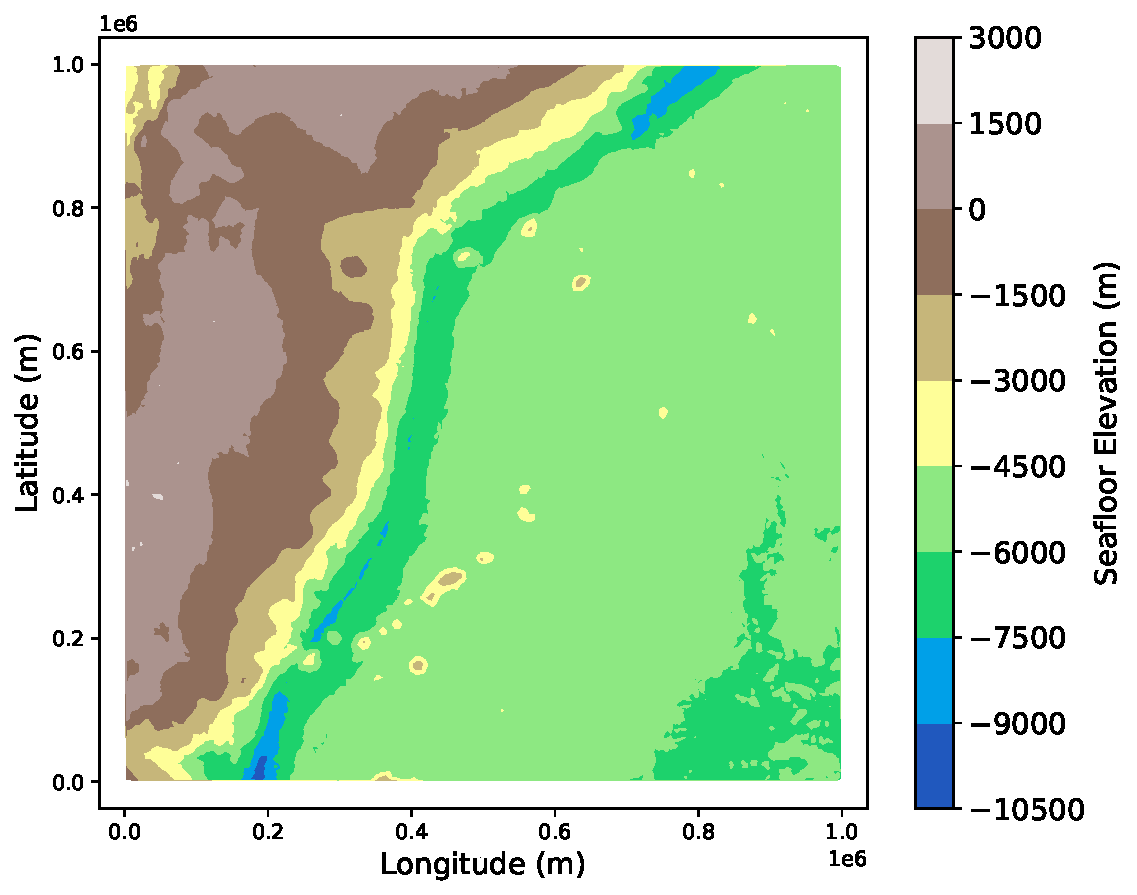
\includegraphics[width=0.65\textwidth]{Figuers/bed_elevation_raw.pdf} % Adjust width as needed
    \centering
    \caption{\scriptsize Bathymetry and Topography of the Computational Domain for the 2011 Tohoku Tsunami Simulations}
    \label{fig:bed_elevation}
\end{figure}

% Reference the figure in your text
As shown in Figure~\ref{fig:bed_elevation}, Bathymetry of the Computational Domain for the 2011 Tohoku Tsunami simulations. Before the earthquake, the water surface is assumed to be at rest, with an undisturbed sea level and no initial flow:

\begin{equation}
h(\textbf{x}, 0) = 0, \quad u(\textbf{x}, 0) = 0, \quad v(\textbf{x}, 0) = 0.
\label{eq:swe-initial-prequake}
\end{equation}
To model the seafloor deformation caused by the earthquake, we use the Okada displacement model \citep{okada1992internal}, which provides an analytical solution for surface deformation due to fault slip in an elastic half-space. This model computes the coseismic displacement \( \Delta z_b(\textbf{x}) \) based on key fault parameters that define the fault geometry and slip characteristics. The \textbf{depth} represents how deep the fault's top edge is below the surface, while the \textbf{length} and \textbf{width} describe the along-strike and down-dip dimensions of the fault plane. The \textbf{slip} quantifies the magnitude of displacement along the fault, whereas the \textbf{strike} specifies the fault's orientation relative to north, measured in degrees. The \textbf{dip} represents the inclination angle of the fault plane relative to a horizontal surface, while the \textbf{rake} defines the direction of slip along the fault plane. Together, these parameters determine the vertical displacement field, shaping the seafloor uplift or subsidence that drives tsunami generation. The earthquake's epicenter location is defined by its \textbf{\( x \)-coordinate} and \textbf{\( y \)-coordinate}, determining the origin of the deformation. Given these parameters, the Okada model computes the vertical displacement field \( \Delta z_b(x) \), representing the seafloor uplift or subsidence that alters the initial seabed topography. This deformation is incorporated into the model as:

\begin{equation}
z_b(\textbf{x}, 0) = z_{b0}(\textbf{x}) + \Delta z_b(\textbf{x}),
\end{equation}

where \( z_{b0}(\textbf{x}) \) represents the original seabed elevation before the earthquake, and \( \Delta z_b(\textbf{x}) \) accounts for the vertical displacement caused by the seismic event. This sudden deformation of the seabed displaces the overlying water column, generating the initial tsunami wave. The resulting modification of the water depth is expressed as:

\begin{equation}
h(\textbf{x}, 0) = \Delta z_b(\textbf{x}), \quad u(\textbf{x}, 0) = 0, \quad v(\textbf{x}, 0) = 0.
\label{eq:swe-initial}
\end{equation}

Thus, the initial tsunami wave is entirely defined by the seafloor deformation \( \Delta z_b(\textbf{x}) \), while the velocity field remains zero, assuming no initial horizontal flow. In this framework, the distributed coseismic deformation \( \Delta z_b(\textbf{x}) \) serves as the input parameter \( p \), which varies spatially over the domain \( \mathcal{X} \). 


% \textcolor{red}{This parameter is integrated into the input representation \( a(\textbf{x}, t, p) \) for the neural operator \( \mathcal{G}_\theta \), enabling the Sensitivity-Constrained Neural Operator (SC-FNO) to model tsunami propagation under realistic earthquake-induced deformations.}



\subsection*{Finite Volume Method for Shallow Water Equations}
\label{sec:fv_sw}

We developed dTSUNAMI, a finite volume solver for the 2D shallow water equations (SWE), designed to efficiently handle tsunami propagation and inundation over complex bathymetry. The solver operates on an unstructured triangular mesh, ensuring mass conservation and allowing for local refinements in regions of interest, such as coastal areas and tsunami impact zones. The governing equations are expressed in their integral form over a control volume \( \Omega_i \):

\begin{equation}
\frac{d}{dt} \int_{\Omega_i} \mathbf{U} \, d\Omega
+ \oint_{\partial \Omega_i} \mathbf{F} \cdot \mathbf{n} \, dS
=
\int_{\Omega_i} \mathbf{S} \, d\Omega,
\end{equation}

where \( \mathbf{U} = (h, hu, hv)^T \) is the conserved state vector, \( \mathbf{F} \) is the flux tensor, \( \mathbf{n} \) is the outward unit normal at each face, and \( \mathbf{S} \) represents source terms.
To enhance accuracy in tsunami simulations, we developed a robust mesh generation approach within dTSUNAMI, leveraging GMSH to create an unstructured triangular mesh with adaptive local refinement.

Fluxes across cell faces are computed using a Riemann solver. We employ the HLLC (Harten-Lax-van Leer-Contact) scheme, which provides a balance between accuracy and robustness. The approximate Riemann solution at an interface is given by:

\begin{equation}
\mathbf{F}_{i+1/2} = 
\begin{cases}
\mathbf{F}_L, & \text{if } S_L \geq 0, \\[5pt]
\mathbf{F}^*, & \text{if } S_L < 0 < S_R, \\[5pt]
\mathbf{F}_R, & \text{if } S_R \leq 0,
\end{cases}
\end{equation}

where \( S_L \) and \( S_R \) are the wave speeds estimated from the characteristic structure of the system.

Time integration is performed using an adaptive second-order Heun’s method, an explicit two-stage Runge-Kutta scheme:

\begin{equation}
\mathbf{K}_1 = \mathbf{F}(t_n, \mathbf{U}_n),
\end{equation}

\begin{equation}
\widetilde{\mathbf{U}}_n = \mathbf{U}_n + \Delta t_n \mathbf{K}_1,
\end{equation}

\begin{equation}
\mathbf{K}_2 = \mathbf{F}(t_n + \Delta t_n, \widetilde{\mathbf{U}}_n),
\end{equation}

\begin{equation}
\mathbf{U}_{n+1} = \mathbf{U}_n + \frac{\Delta t_n}{2} (\mathbf{K}_1 + \mathbf{K}_2).
\end{equation}

The time step \( \Delta t_n \) is adaptively chosen based on the Courant-Friedrichs-Lewy (CFL) condition.



% There are $308,001$ triangular cells and $154,598$ nodes for the mesh, generating a high-resolution simulation of the tsunami waves for training. We coarsened this solution and its Jacobians to $100\times100$ for neural operator training. 



We validated dTSUNAMI against the 2011 Tohoku tsunami, triggered by the Mw 9.0 earthquake that occurred on March 11, 2011, at 05:46 UTC (14:46 JST), with its epicenter located at 37.490°\,N, 143.030°\,E. 

The computational domain employs an unstructured triangular mesh consisting of 308,001 cells and 154,598 nodes. Figure~\ref{fig:tohoku_validation} shows time series of the simulated free-surface elevation compared to measurements recorded at the North Miyagi offshore GPS wave gauge (station 803) of the NOWPHAS network. For reference, the same figure includes the results reported by Grilli et al.~\citep{grilli2013numerical} using the Boussinesq model FUNWAVE-TVD. 



\begin{figure}[htbp]
\centering
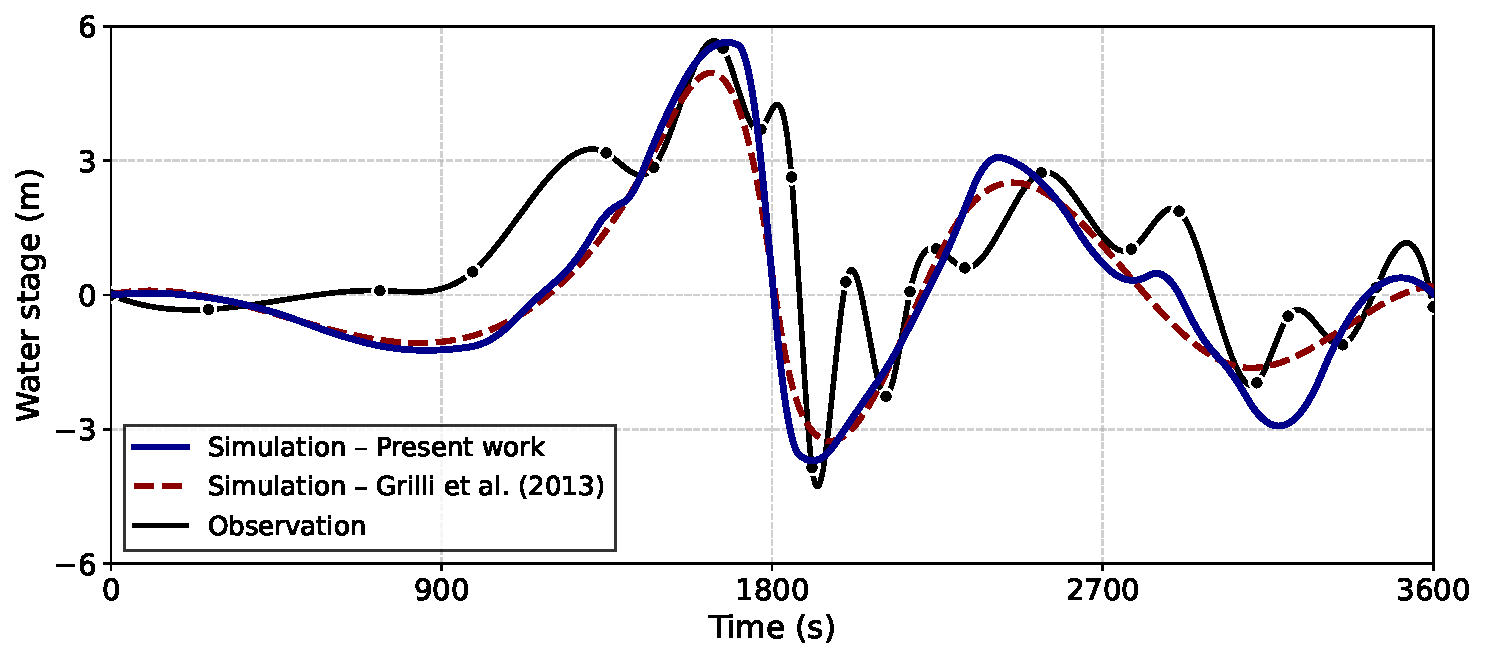
\includegraphics[width=0.9\textwidth]{Figuers/validation_gauge_g.pdf}
\caption{\scriptsize Comparison of simulated free-surface elevation time series at North Miyagi offshore GPS wave gauge (station 803, NOWPHAS network) with recorded measurements during the 2011 Tohoku tsunami.}
\label{fig:tohoku_validation}
\end{figure}


The dTSUNAMI results exhibit very good agreement with both the observed data and the reference simulation, accurately capturing the arrival time, amplitude of the leading crest, and the subsequent wave train. This close match clearly demonstrates the validity and high accuracy of the solver for real-world large-scale tsunami propagation simulations.







\subsection*{Adjoint-Based Sensitivity Computation}
\label{sec:adjoint_sensitivity}

To quantify the sensitivity of the final water depth \( h_N \) to variations in bed topography \( b \), we employ the adjoint method. This approach efficiently computes gradients without requiring finite-difference perturbations, making it well-suited for high-dimensional tsunami simulations.

\subsubsection*{Adjoint System Formulation}

The forward SWE system evolves as:
\begin{equation}
\mathbf{U}_{n+1} = \mathbf{U}_n + \frac{\Delta t_n}{2} \left( \mathbf{K}_1^n + \mathbf{K}_2^n \right),
\end{equation}
where
\begin{equation}
\mathbf{K}_1^n = \mathbf{F}(\mathbf{U}_n, \mathbf{b}), \quad
\mathbf{K}_2^n = \mathbf{F}(\widetilde{\mathbf{U}}_n, \mathbf{b}),
\end{equation}
and the final objective function is:
\begin{equation}
J = \mathbf{h}_N = \mathbf{P} \mathbf{U}_N,
\end{equation}
where \( \mathbf{P} \) extracts water depth \( h \) from \( \mathbf{U} \).

The Lagrangian function incorporates the constraints imposed by the forward dynamics:
\begin{align}
\mathcal{L} = J + \sum_{n=0}^{N-1} \bigg[
\boldsymbol{\lambda}_{1,n}^T \left( \mathbf{K}_1^n - \mathbf{F}(\mathbf{U}_n, \mathbf{b}) \right)
+ \boldsymbol{\lambda}_{2,n}^T \left( \widetilde{\mathbf{U}}_n - \mathbf{U}_n - \Delta t_n \mathbf{K}_1^n \right)  \notag \\
+ \boldsymbol{\lambda}_{3,n}^T \left( \mathbf{K}_2^n - \mathbf{F}(\widetilde{\mathbf{U}}_n, \mathbf{b}) \right)
+ \boldsymbol{\lambda}_{4,n}^T \left( \mathbf{U}_{n+1} - \mathbf{U}_n - \frac{\Delta t_n}{2} (\mathbf{K}_1^n + \mathbf{K}_2^n) \right) \bigg].
\end{align}

\subsubsection*{Backward Recursive Computation of Adjoint Variables}

The adjoint system is solved by backward recursion, starting from the final time step.

\textbf{Initialization at Final Time Step:}
\begin{equation}
\boldsymbol{\lambda}_{4,N-1} = -\mathbf{P}^T.
\end{equation}

\textbf{Recursive Computation for \( n = N-1, N-2, \dots, 0 \):}
\begin{enumerate}
    \item Compute adjoint correction for \( \mathbf{K}_2^n \):
    \begin{equation}
    \boldsymbol{\lambda}_{3,n} = \frac{\Delta t_n}{2} \boldsymbol{\lambda}_{4,n}.
    \end{equation}

    \item Compute adjoint variable for the intermediate state \( \widetilde{\mathbf{U}}_n \):
    \begin{equation}
    \boldsymbol{\lambda}_{2,n} = \boldsymbol{\lambda}_{3,n}^T \frac{\partial \mathbf{F}}{\partial \mathbf{U}} \Big|_{\widetilde{\mathbf{U}}_n}.
    \end{equation}

    \item Compute adjoint correction for \( \mathbf{K}_1^n \):
    \begin{equation}
    \boldsymbol{\lambda}_{1,n} = \Delta t_n \boldsymbol{\lambda}_{2,n} + \frac{\Delta t_n}{2} \boldsymbol{\lambda}_{4,n}.
    \end{equation}

    \item Update adjoint state for the next iteration:
    \begin{equation}
    \boldsymbol{\lambda}_{4,n-1} = \boldsymbol{\lambda}_{1,n} \frac{\partial \mathbf{F}}{\partial \mathbf{U}} \Big|_{\mathbf{U}_n} + \boldsymbol{\lambda}_{2,n} + \boldsymbol{\lambda}_{4,n}.
    \end{equation}
\end{enumerate}
The recursive computation of \(\boldsymbol{\lambda}\) proceeds from the final time step \(N\) back to the initial time step \(0\). The pseudocode for efficient implementation of the recursion is presented in Algorithm~\ref{alg:adjoint}.


\begin{algorithm}[H]
\caption{Recursive Computation of \(\boldsymbol{\lambda}\)}
\label{alg:adjoint}
\begin{algorithmic}[1]
    \State \textbf{Input:} 
    \begin{itemize}
        \item Time steps \(\Delta t_n\)
        \item Jacobians \(\frac{\partial \mathbf{F}}{\partial \mathbf{b}}\big|_{\mathbf{U}_n}\), \(\frac{\partial \mathbf{F}}{\partial \mathbf{b}}\big|_{\widetilde{\mathbf{U}}_n}\)
        \item Output matrix \(\mathbf{P}\)
    \end{itemize}
    \State \textbf{Initialize:} 
    \[
    \boldsymbol{\lambda}_{4,N-1} \gets -\mathbf{P}^T
    \]
    \For{\(n = N-1, N-2, \dots, 0\)}
        \State \textbf{Step 1: Compute \(\boldsymbol{\lambda}_{3,n}\)}
        \[
        \boldsymbol{\lambda}_{3,n} \gets \frac{\Delta t_n}{2} \boldsymbol{\lambda}_{4,n}
        \]

        \State \textbf{Step 2: Compute \(\boldsymbol{\lambda}_{2,n}\)}
        \[
        \boldsymbol{\lambda}_{2,n} \gets \boldsymbol{\lambda}_{3,n}^T \frac{\partial \mathbf{F}}{\partial \mathbf{U}} \big|_{\widetilde{\mathbf{U}}_n}
        \]

        \State \textbf{Step 3: Compute \(\boldsymbol{\lambda}_{1,n}\)}
        \[
        \boldsymbol{\lambda}_{1,n} \gets \Delta t_n \boldsymbol{\lambda}_{2,n} + \frac{\Delta t_n}{2} \boldsymbol{\lambda}_{4,n}
        \]

        \State \textbf{Step 4: Update \(\boldsymbol{\lambda}_{4,n-1}\)}
        \[
        \boldsymbol{\lambda}_{4,n-1} \gets \boldsymbol{\lambda}_{1,n} \frac{\partial \mathbf{F}}{\partial \mathbf{U}} \big|_{\mathbf{U}_n} + \boldsymbol{\lambda}_{2,n} + \boldsymbol{\lambda}_{4,n}
        \]

        \State \textbf{Step 5: Store Intermediate Values:}
        \begin{itemize}
            \item Save \(\boldsymbol{\lambda}_{1,n}\) for sensitivity computation
            \item Save \(\boldsymbol{\lambda}_{3,n}\) for sensitivity computation
        \end{itemize}
    \EndFor
\end{algorithmic}
\end{algorithm}

The final sensitivity of the water depth at \( t = T \) with respect to bed topography is obtained as:

\begin{equation}
\frac{\partial J}{\partial b} = \sum_{n=0}^{N-1} \left[
-\boldsymbol{\lambda}_{1,n}^T \frac{\partial \mathbf{F}}{\partial b} \Big|_{\mathbf{U}_n}
- \boldsymbol{\lambda}_{3,n}^T \frac{\partial \mathbf{F}}{\partial b} \Big|_{\widetilde{\mathbf{U}}_n}
\right].
\end{equation}

Since \( J = \mathbf{h}_N = \mathbf{P} \mathbf{U}_N \), we obtain:

\begin{equation}
\frac{\partial h_N}{\partial b} = \sum_{n=0}^{N-1} \left[
-\boldsymbol{\lambda}_{1,n}^T \frac{\partial \mathbf{F}}{\partial b} \Big|_{\mathbf{U}_n}
- \boldsymbol{\lambda}_{3,n}^T \frac{\partial \mathbf{F}}{\partial b} \Big|_{\widetilde{\mathbf{U}}_n}
\right].
\end{equation}

This Jacobian \( \frac{\partial h_N}{\partial b} \in \mathbb{R}^{M \times M} \) quantifies how changes in bed topography influence final water depth, crucial for tsunami inversion and forecasting.


\subsubsection*{Derivation of $\frac{\partial \mathbf{F}}{\partial \mathbf{U}}$ for FVM}
To compute the adjoint sensitivity, we derive the local Jacobian \( \frac{\partial \mathbf{F}}{\partial \mathbf{U}} \) for the finite volume discretization. Differentiating the numerical flux at a face shared between cells \( i \) and \( j \):

\begin{equation}
\frac{\partial \mathbf{F}_f}{\partial \mathbf{U}_i} =
\begin{pmatrix}
\mathbf{u} \cdot \mathbf{n} & n_x & n_y \\
u (\mathbf{u} \cdot \mathbf{n}) + g h n_x & 2 u n_x & u n_y \\
v (\mathbf{u} \cdot \mathbf{n}) + g h n_y & v n_x & 2 v n_y
\end{pmatrix}.
\end{equation}

For source terms including bed slope and friction:
\begin{equation}
\frac{\partial \mathbf{S}_i}{\partial \mathbf{U}_i} =
\begin{pmatrix}
0 & 0 & 0 \\
- g \frac{\partial b}{\partial x} - c_f u & -c_f |\mathbf{u}| & 0 \\
- g \frac{\partial b}{\partial y} - c_f v & 0 & -c_f |\mathbf{u}|
\end{pmatrix},
\end{equation}
where \( c_f = g n^2 / h^{4/3} \) is the friction coefficient.

\paragraph{Jacobian Assembly}
The full local Jacobian is assembled as:
\begin{equation}
\frac{\partial \mathbf{F}_i}{\partial \mathbf{U}_i} = -\frac{1}{A_i} \sum_{f \in \text{faces}(i)} l_f \frac{\partial \mathbf{F}_f}{\partial \mathbf{U}_i} + \frac{\partial \mathbf{S}_i}{\partial \mathbf{U}_i}.
\end{equation}
For neighboring cell interactions:
\begin{equation}
\frac{\partial \mathbf{F}_i}{\partial \mathbf{U}_j} = \frac{1}{A_i} l_f \frac{\partial \mathbf{F}_f}{\partial \mathbf{U}_j}, \quad j \in \text{neighbors}(i).
\end{equation}

This formulation ensures consistency with the adjoint framework, capturing local sensitivities required for gradient-based inversion and optimization.




\subsubsection*{Derivation of $\frac{\partial \mathbf{F}}{\partial b}$ for FVM}
To compute the local sensitivity of the shallow water system to bed topography \( b \), we differentiate the right-hand side function \( \mathbf{F} \).

\paragraph{Flux Contributions}
The governing equations include:
\begin{align}
\frac{\partial \mathbf{F}_1}{\partial b} &= 0, \\[5pt]
\frac{\partial \mathbf{F}_2}{\partial b} &= -gh \frac{\partial b}{\partial x}, \\[5pt]
\frac{\partial \mathbf{F}_3}{\partial b} &= -gh \frac{\partial b}{\partial y}.
\end{align}
Only the momentum equations contain explicit \( b \)-dependence via the bed slope terms.

For a domain with \( M \) cells, the Jacobian matrix is:
\begin{equation}
\frac{\partial \mathbf{F}}{\partial b} =
\begin{pmatrix}
\mathbf{0}_{M \times M} \\[5pt]
- g \text{diag}(h) \cdot \text{diag}(S_x) \\[5pt]
- g \text{diag}(h) \cdot \text{diag}(S_y)
\end{pmatrix} \in \mathbb{R}^{3M \times M}.
\end{equation}

In this formulation, the first \( M \) rows correspond to continuity equations with no explicit \( b \)-dependence. The middle and last \( M \) rows represent the effects of bed slope on x- and y-momentum equations, respectively. The diagonal form ensures each grid cell's sensitivity is localized, aligning with the adjoint system.



\subsection*{Neural Operator Learning for the Shallow Water Equations}

We employ neural operator learning to model tsunami dynamics governed by the shallow water equations with Manning friction, applied to the 2011 Tohoku event setup. Variability across samples arises from earthquake-induced seafloor deformation, represented through the Okada dislocation framework. Okada fault parameters are sampled within the ranges reported in \citep{grilli2013numerical}, and random earthquake epicenters are assigned as illustrated in Supplementary Fig.~\ref{fig:nse_sampling_strategies}.  

To generate training data, we used the dTSUNAMI finite volume solver on an unstructured triangular mesh consisting of 308,001 cells and 154,598 nodes. Each simulation is run for 3600 seconds, storing 51 uniformly spaced snapshots. These high-resolution solutions and their Jacobians are subsequently coarsened to a 100×100 uniform grid for neural operator training.

Within the SC-NO framework, the input function consists of the first $t_u = 5$ time steps of the water stage field $h(\mathbf{x}, t)$ together with the seafloor deformation $\Delta z_b(\mathbf{x})$ computed from the Okada model. The neural operator $\mathcal{G}_\theta$ is then trained to predict the remaining $t_G = 46$ time steps, guided by the Jacobian of the final water stage with respect to the bed topography, computed via the adjoint method (Supplementary Section~\ref{sec:adjoint_sensitivity}). Formally, the operator learning problem is defined as:
\begin{equation}
\mathcal{G}_\theta : \left( \mathcal{X} \times [0, t_u], \, \Delta z_b(\mathbf{x}) \right) \;\to\; h(\mathbf{x}, t, \Delta z_b), 
\quad \text{for } (\mathbf{x}, t) \in \mathcal{X} \times [t_u, T].
\end{equation}

To evaluate both interpolation and extrapolation performance, we consider two testing scenarios: (i) an \textit{in-training} case, where earthquake epicenters fall within the range covered by the training set, and (ii) an \textit{out-of-training} case, where epicenters lie outside this region (Supplementary Fig.~\ref{fig:nse_sampling_strategies}). This setup enables us to assess not only the accuracy of SC-NO within the training distribution but also its ability to generalize tsunami propagation to previously unseen earthquake configurations, serving as an out-of-distribution (OOD) evaluation.  


This approach integrates spatial-temporal input information with earthquake source parameters, enabling SC-NO to learn a solution operator that generalizes tsunami propagation and inundation across both in-training and out-of-distribution epicenter scenarios.  


\begin{figure}[!ht]
    \centering
    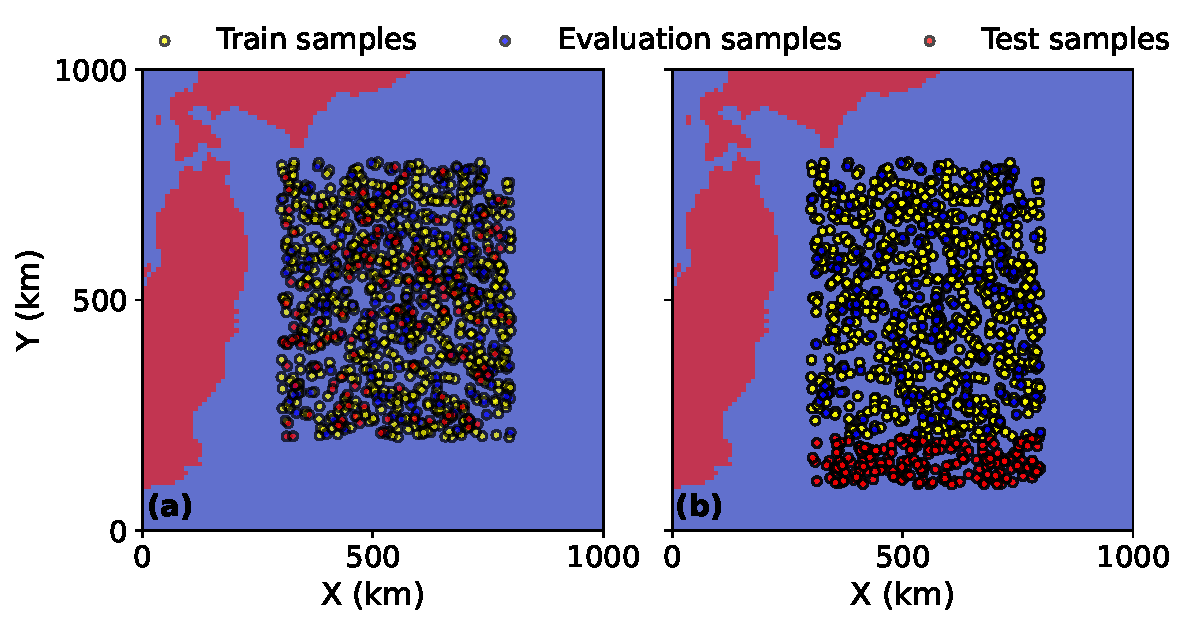
\includegraphics[width=0.8\textwidth]{Figuers/sampling_strategy.pdf}

    \caption{\scriptsize\textbf{Sampling strategy for PDE3 (tsunami scenario).} 
    (a) Training and evaluation samples are generated from random earthquake epicenters distributed across the central region of the domain. 
    (b) Out-of-distribution (OOD) test samples are generated by shifting epicenters into a geographically distinct southern band, ensuring that all test events occur in a region not represented in the training or evaluation sets.}     
        
        \label{fig:nse_sampling_strategies}
\end{figure}




\subsection*{Mapping Between Fine Solver Mesh and Coarse Neural Operator Grid}
\label{sec:coarse_fine_mapping}

For the shallow-water tsunami case (PDE3), neural operator training and inference are conducted on a fixed $100\times100$ uniform grid, while the governing dynamics are solved on a substantially finer unstructured mesh using the dTSUNAMI finite volume solver. This resolution disparity requires two complementary mappings: a \emph{coarsening} operator that restricts high-resolution solutions to the learning grid, and an \emph{upscaling} operator that reconstructs physically consistent fine-scale fields from coarse neural-operator predictions.

\paragraph{Coarsening of fine-scale solutions.}
Let $d(\mathbf{x}, t)$ denote the fine-scale water depth field produced by the solver on the continuous domain $\mathcal{X}$. We introduce a uniform partition $\{\Omega_{ij}\}$ of $\mathcal{X}$ corresponding to the $100\times100$ neural operator grid. Coarsening is performed via a cell-averaging operator,
\begin{equation}
\bar{d}_{ij}(t)
=
\frac{1}{|\Omega_{ij}|}
\int_{\Omega_{ij}} d(\mathbf{x}, t)\, d\mathbf{x},
\end{equation}
yielding a coarse depth field $\bar{d}_{ij}(t)$ that preserves the mean water depth within each cell. In practice, this corresponds to averaging solver values associated with fine mesh elements whose centroids lie within $\Omega_{ij}$. This projection provides a physically consistent low-resolution representation suitable for neural operator learning while retaining the dominant large-scale dynamics.




\paragraph{Physically based upscaling from coarse to fine resolution.}
The inverse mapping from coarse mean depth to fine-scale depth is not uniquely defined: many fine configurations yield the same coarse average. To obtain a physically meaningful reconstruction, the upscaling is defined as a \emph{cell-wise hydrostatic fill} over the known fine bathymetry.

Let $\{\Omega_{ij}\}$ denote the $100\times 100$ coarse partition of the horizontal domain, and let $\{(\mathbf{x}_p,z_{b,p})\}_{p=1}^{N}$ be the fine solver nodes (or vertices), where $\mathbf{x}_p\in\mathbb{R}^2$ and $z_{b,p}=z_b(\mathbf{x}_p)$ is the bed elevation. Each fine node is assigned to exactly one coarse cell via
\begin{equation}
c(p)= (i,j)\quad \text{s.t.}\quad \mathbf{x}_p\in\Omega_{ij}, 
\qquad 
\mathcal{P}_{ij}=\{p:\,c(p)=(i,j)\},\quad N_{ij}=|\mathcal{P}_{ij}|.
\end{equation}
The neural operator predicts the coarse mean depth $\bar d_{ij}(t)$ on each cell. The reconstructed fine depth is defined pointwise by
\begin{equation}
d_p(t) \;=\; \big(H_{ij}(t)-z_{b,p}\big)_+,
\qquad p\in\mathcal{P}_{ij},
\qquad (a)_+ := \max(a,0),
\label{eq:bathtub_pointwise}
\end{equation}
where $H_{ij}(t)$ is a \emph{cell-wise water level} (stage) chosen to satisfy the coarse mean-depth constraint in \emph{discrete} form:
\begin{equation}
\frac{1}{N_{ij}}\sum_{p\in\mathcal{P}_{ij}} \big(H_{ij}(t)-z_{b,p}\big)_+ \;=\; \bar d_{ij}(t).
\label{eq:bathtub_mean_constraint}
\end{equation}
Equation~\eqref{eq:bathtub_mean_constraint} defines $H_{ij}(t)$ implicitly. The left-hand side is a continuous, non-decreasing function of $H_{ij}(t)$, hence the solution exists and is unique whenever $\bar d_{ij}(t)$ is attainable over the local bathymetric distribution $\{z_{b,p}\}_{p\in\mathcal{P}_{ij}}$. In practice, $H_{ij}(t)$ is obtained by bisection with brackets
\begin{equation}
H_{ij}^{\mathrm{low}} = \min_{p\in\mathcal{P}_{ij}} z_{b,p},
\qquad
H_{ij}^{\mathrm{high}} = \max_{p\in\mathcal{P}_{ij}} z_{b,p} + \bar d_{ij}(t) + \varepsilon,
\end{equation}
and the cell is treated as dry whenever $\bar d_{ij}(t)\le d_{\min}$, in which case $d_p(t)=0$ for all $p\in\mathcal{P}_{ij}$.

Finally, to ensure that the reconstruction preserves the \emph{total} water volume implied by the coarse prediction at each time $t$, an optional per-time-step global rescaling is applied. Let $A_{ij}=|\Omega_{ij}|$ be the coarse cell area and approximate each node in $\Omega_{ij}$ by an equal area weight $A_{ij}/N_{ij}$. Then the target and reconstructed volumes are
\begin{equation}
V_{\mathrm{target}}(t)=\sum_{i,j} \bar d_{ij}(t)\,A_{ij},
\qquad
V_{\mathrm{rec}}(t)=\sum_{i,j}\sum_{p\in\mathcal{P}_{ij}} d_p(t)\,\frac{A_{ij}}{N_{ij}},
\end{equation}
and we set a scalar factor $\alpha(t)=V_{\mathrm{target}}(t)/V_{\mathrm{rec}}(t)$ (when $V_{\mathrm{rec}}(t)>0$) and replace $d_p(t)\leftarrow \alpha(t)\,d_p(t)$.
This upscaling is therefore non-negative, bathymetry-aware, and exactly consistent with the coarse mean-depth constraints by construction, while avoiding the unphysical shoreline behavior that can arise from purely geometric interpolation in shallow regions.



\begin{figure}[!ht]
    \centering
    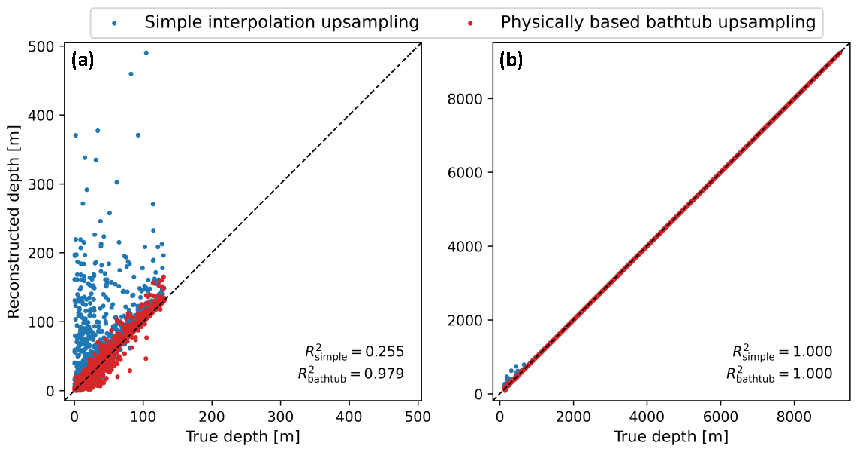
\includegraphics[width=0.9\textwidth]{Figuers/upsampling_error.pdf}
    \caption{\scriptsize\textbf{Comparison of depth upscaling methods.}
    (a) Shallow-water regime (0--5th percentile of true depth).
    (b) Moderate-to-deep regime (5--100th percentile of true depth).}
    \label{fig:upsampling_comparison}
\end{figure}




A common alternative is to upsample coarse predictions using standard interpolation methods (e.g., nearest-neighbor or bilinear interpolation of depth or stage). Such approaches ignore bathymetric variability and do not enforce physical constraints, often leading to spurious inundation over dry land and degraded accuracy in shallow regions.

Figure~\ref{fig:upsampling_comparison} illustrates a controlled comparison between a standard interpolation-based reconstruction and the proposed physically based upscaling procedure. Starting from a high-resolution reference solution obtained from the tsunami solver, the water depth field is first \emph{coarsened} to the $100\times100$ uniform grid used by the neural operator. This coarse representation is then independently upscaled back to the original fine resolution using (i) a purely geometric interpolation scheme and (ii) the proposed bathtub-based reconstruction. The resulting reconstructed fields are compared against the original high-resolution solution.

In shallow-water regions near the shoreline (0–5th percentile of true depth), interpolation-based reconstruction fails to recover physically meaningful depths and exhibits poor agreement with the reference solution (Figure~\ref{fig:upsampling_comparison}a). This failure arises because interpolation does not account for local bathymetric structure and cannot enforce essential physical constraints such as non-negativity of depth or shoreline emergence. In contrast, the bathtub-based reconstruction explicitly incorporates the underlying bed elevation and enforces consistency with the coarse mean depth, yielding accurate recovery of shallow-water states.

In moderate-to-deep regions, both reconstruction approaches perform comparably well, indicating that simple interpolation is sufficient only away from the shoreline (Figure~\ref{fig:upsampling_comparison}b). These results demonstrate that physically informed upscaling is a necessary complement to coarse neural-operator predictions when reconstructing near-shore and inundation-relevant tsunami dynamics, while purely geometric interpolation is inadequate in depth regimes most critical for hazard assessment.
Taken together, this comparison establishes the upscaling procedure as a reliable and physically consistent complement to the neural-operator framework. While SC-NO is trained and evaluated entirely on coarse-resolution fields, the proposed reconstruction enables faithful recovery of fine-scale depth distributions required for solver-level validation, visualization, and downstream hazard analysis. Importantly, this post-processing step operates independently of the learned operator and does not modify its predictions; instead, it provides a principled bridge between coarse neural-operator outputs and high-resolution physical fields, ensuring consistency with bathymetry and shallow-water physics.





\subsection*{Three-Stage Inversion Framework for Tsunami Source Reconstruction}
\label{sec:inversion_framework}

Rapid and reliable estimation of tsunami sources is vital for the effectiveness of real-time early-warning systems. When a major undersea earthquake occurs, the resulting seafloor deformation initiates tsunami waves that can traverse ocean basins and reach coastal regions within minutes, demanding immediate and accurate source characterization.  
To meet this need, we introduce a \textbf{data-driven, gradient-based inversion framework} that integrates \textbf{Neural Operators} with \textbf{Okada surrogate networks} to reconstruct the earthquake-induced seafloor deformation and infer the corresponding fault parameters directly from \textbf{early-stage tsunami gauge observations}.  
These early observations, typically spanning the first 30 minutes after the event onset, contain limited yet highly informative signals that guide the inversion toward physically consistent, interpretable, and computationally efficient source reconstructions suitable for real-time forecasting.
The framework combines the differentiability and efficiency of neural operators with the interpretability of Okada fault parameterization, enabling near--real-time source reconstruction with both accuracy and physical coherence. The inversion proceeds in three sequential stages, progressively transitioning from field-level reconstruction to interpretable parameter refinement (Figure~\ref{fig:inversion_stages}).




\begin{figure}[htbp]
    \centering
    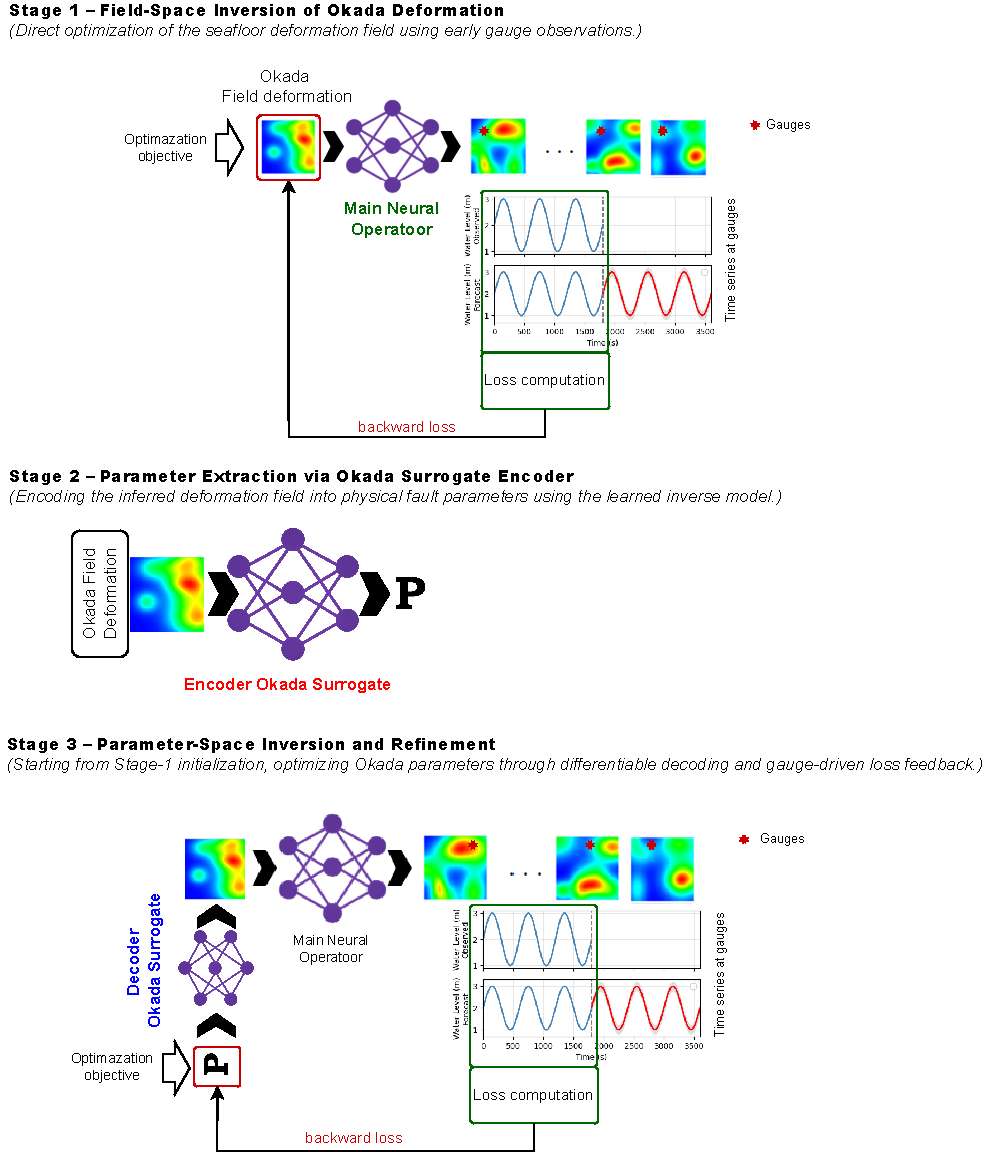
\includegraphics[width=0.98\textwidth, trim={0 0 0 0}, clip]{Figuers/inversion_tsunami.pdf}
    \caption{\scriptsize\textbf{Three-stage tsunami inversion workflow.}  
    The framework integrates neural operator surrogates and Okada-based encoder–decoder networks for rapid and interpretable tsunami source reconstruction.  
    \textbf{Stage~1:} Field-space inversion optimizes the Okada deformation field using early tsunami gauge observations via neural operator surrogates (FNO or SC-FNO).  
    \textbf{Stage~2:} The inferred deformation is passed through a U-FNO--based Okada Surrogate Encoder that maps the 2D field to a nine-dimensional fault parameter vector $\mathbf{P}$.  
    \textbf{Stage~3:} A U-FNO Decoder reconstructs the deformation field from $\mathbf{P}$, enabling parameter-space refinement through differentiable feedback and gauge-driven loss propagation.
    }
    
    \label{fig:inversion_stages}
\end{figure}



\begin{figure}[htbp]
    \centering
    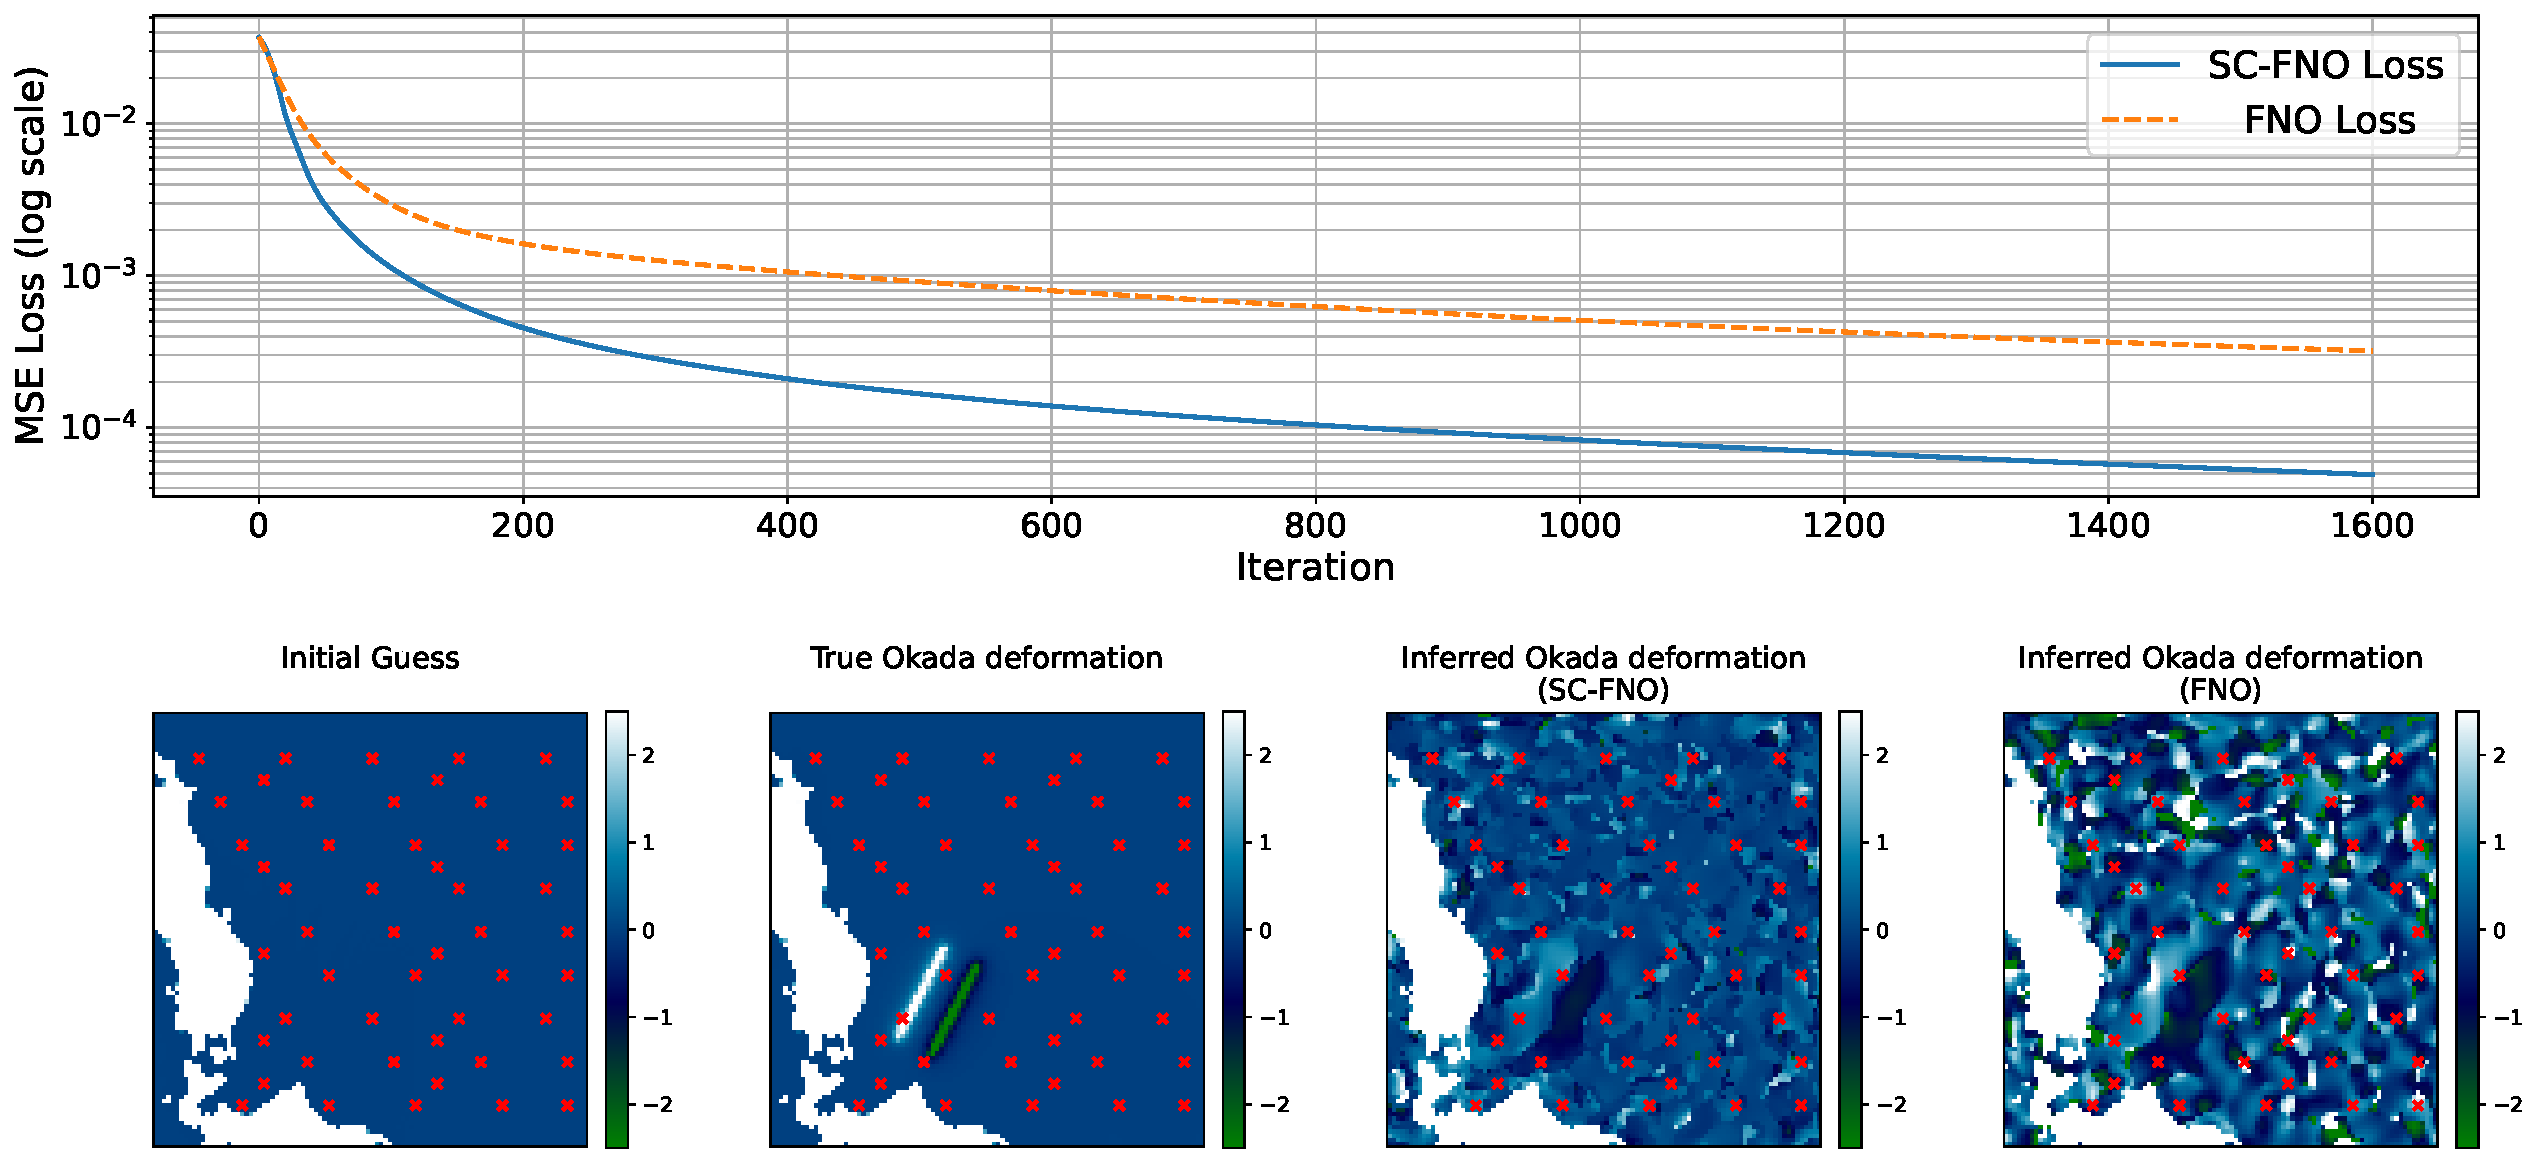
\includegraphics[width=\textwidth, trim={0 0 0 0}, clip]{Figuers/PDE3_inversion_stage_1.pdf}
    \caption{\scriptsize\textbf{Field-space inversion of Okada deformation (Stage~1).}  
    Evolution of the mean squared error (MSE) loss during inversion using SC-FNO and FNO (top), and comparison of deformation fields (bottom).  
    Red dots indicate the locations of tsunami gauges.}
        \label{fig:stage1_field_inversion}
\end{figure}




\paragraph{Stage 1 --- Field-Space Inversion of Okada Deformation}
\textit{(Direct gradient-based optimization of the seafloor deformation field using early gauge observations.)}

In the first stage, inversion is performed directly in the \textbf{field domain} to reconstruct the Okada deformation field---the vertical displacement of the seafloor responsible for tsunami initiation.  
Starting from an initial guess, the deformation field is iteratively updated through gradient descent to minimize the mean squared error between simulated and observed water-stage time series at selected gauge locations during the early event window ($T_u = 30$ minutes).  

Forward simulations are produced by a pretrained Neural Operator---either the baseline FNO or the Sensitivity-Constrained FNO ---which acts as a differentiable surrogate for the shallow water equations.  
This stage yields an initial deformation estimate that reproduces the observed signals but may contain \textbf{low-frequency artifacts} or \textbf{nonphysical features}, since the optimization acts directly on spatial pixels without explicit parameter constraints. At the end of Stage~1, both models converge toward deformation fields that reproduce the early tsunami gauge observations with reasonable accuracy (Figure~\ref{fig:stage1_field_inversion}). Although residual discrepancies remain in both reconstructions, the \textbf{SC-FNO} demonstrates faster convergence, smoother gradients, and more accurate localization of the primary rupture zone compared to the baseline \textbf{FNO}. The SC-FNO–inferred field better captures the overall geometry, polarity, and region of occurrence of the true Okada deformation, while the FNO result remains affected by high-frequency noise and scattered artifacts.  




\paragraph{Stage 2 --- Parameter Extraction via Okada Surrogate Encoder}
\textit{(Encoding the inferred deformation field into compact Okada fault parameters through a learned inverse mapping.)}

To restore physical interpretability, the deformation field recovered in Stage~1, denoted as $\mathbf{F} \in \mathbb{R}^{H \times W}$, is passed through a pretrained \textbf{Okada Surrogate Encoder} $E_{\theta}$.  
This network performs the nonlinear mapping  
\[
E_{\theta} : \mathbf{F} \; \rightarrow \; \mathbf{P} \in \mathbb{R}^{9},
\]
where $\mathbf{P}$ represents the compact vector of Okada fault parameters, including the fault epicenter coordinates ($x$, $y$), depth, length, width, strike, dip, rake, and slip magnitude.



% Although purely data-driven and not physics-informed, this pair effectively approximates the analytical mapping. The encoding step compresses the field inversion result into a physically constrained latent representation, ensuring that subsequent optimization evolves along a \textbf{realistic fault manifold} while suppressing spatial artifacts from Stage~1.



\begin{figure}[htbp]
    \centering
    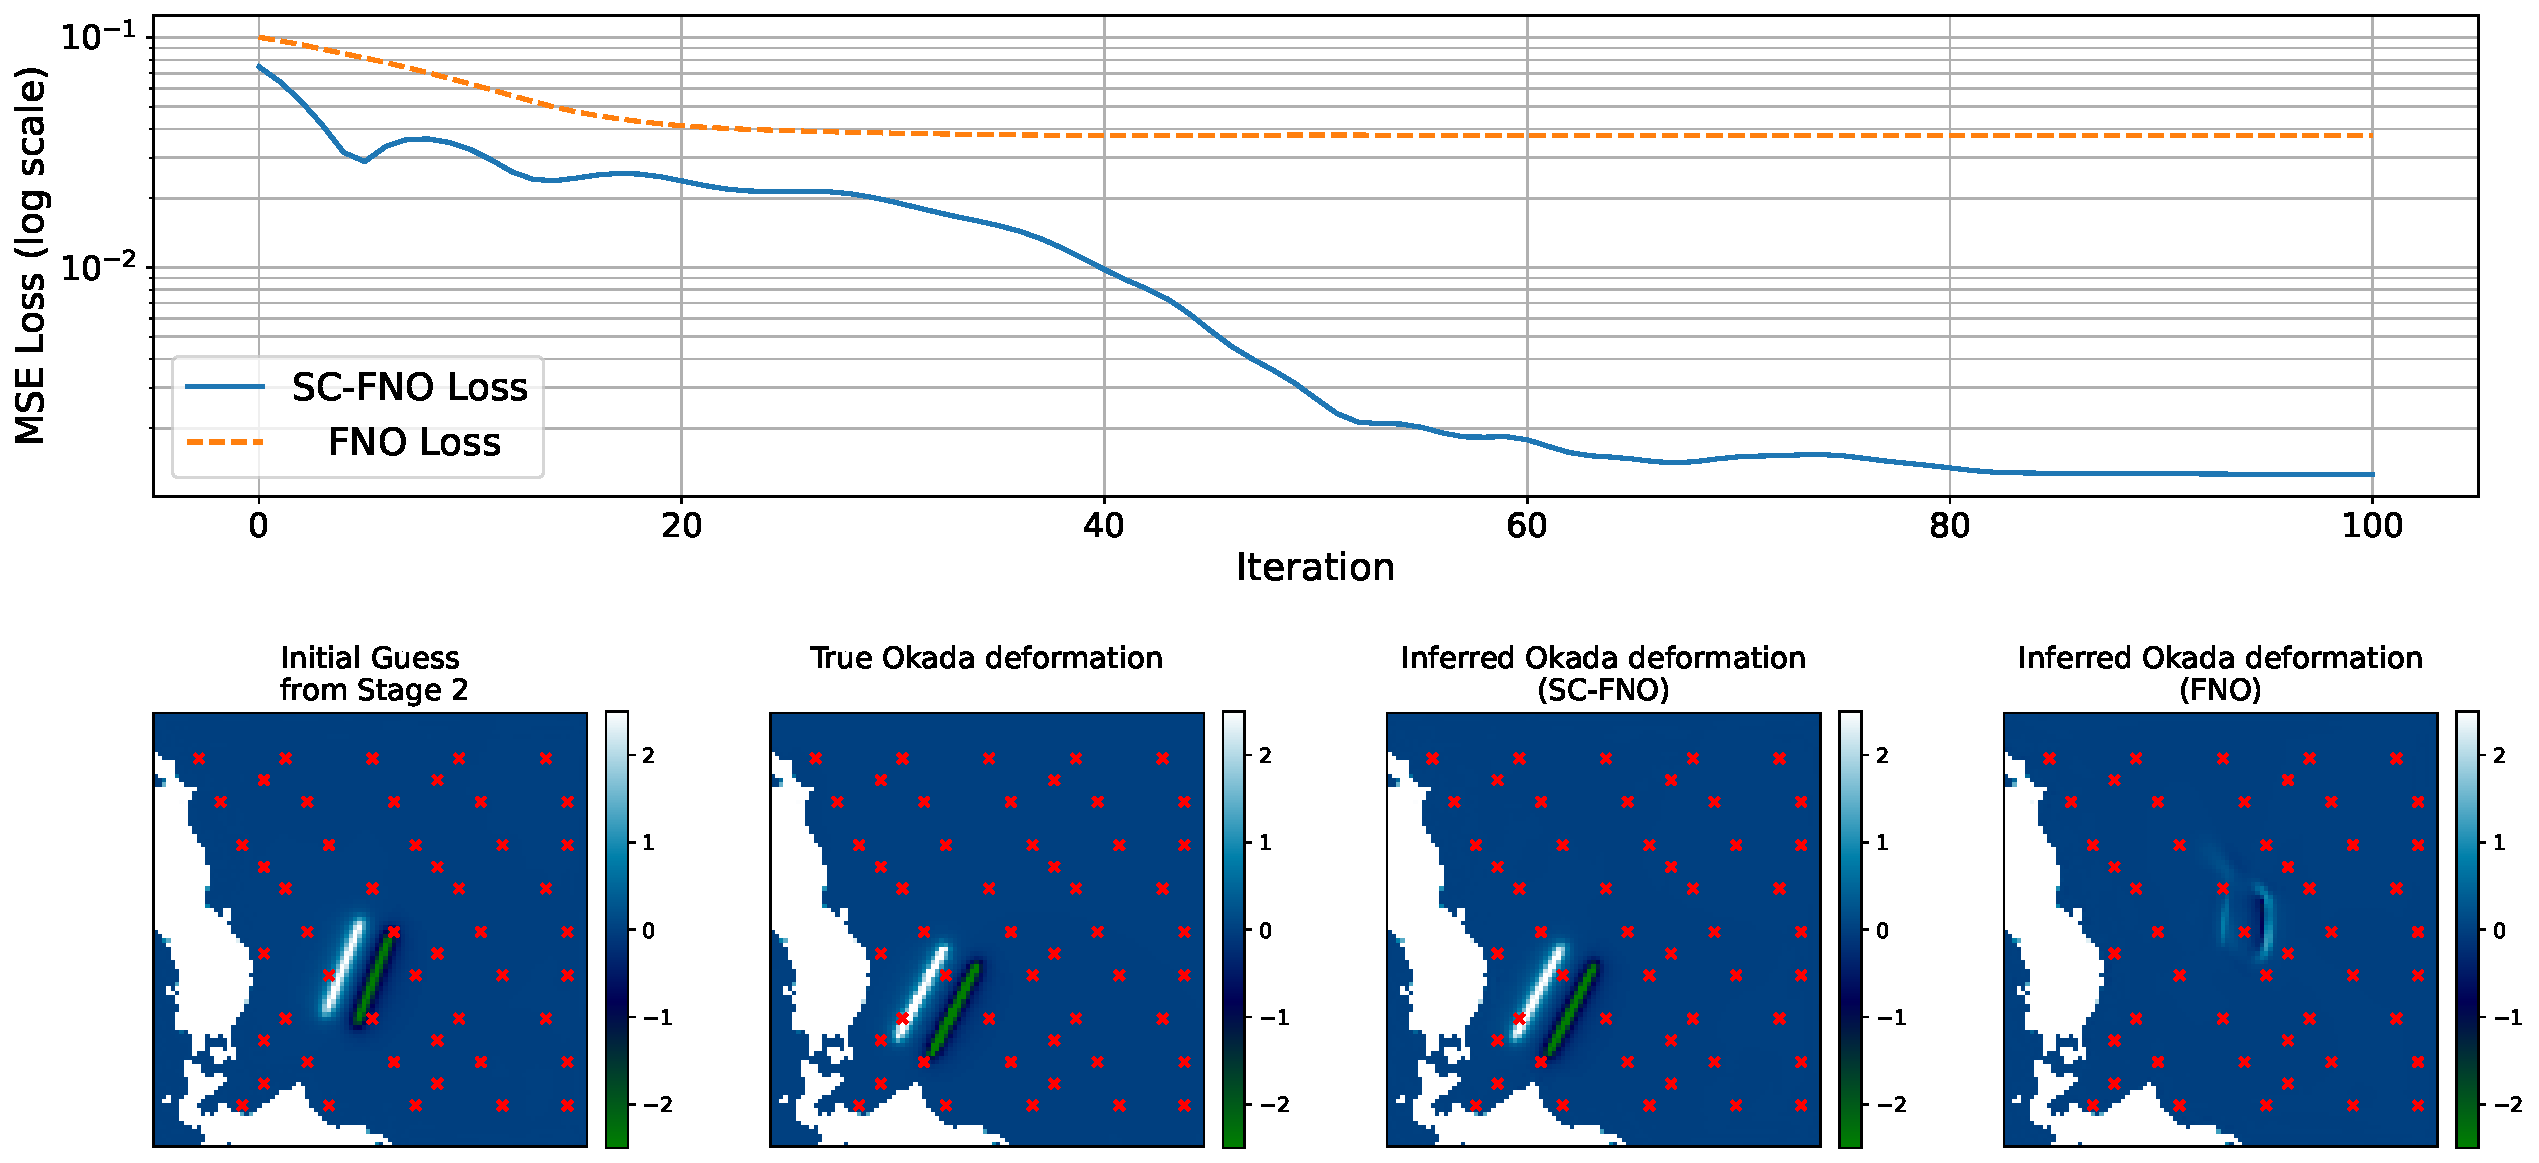
\includegraphics[width=0.98\textwidth, trim={0 0 0 0}, clip]{Figuers/PDE3_inversion_stage_2.pdf}
    \caption{\scriptsize\textbf{Parameter-space inversion and refinement (Stage~3).}  
    Convergence of the mean squared error (MSE) loss during parameter-space optimization (top) and comparison of deformation fields (bottom).  
    The optimization is initialized using parameters inferred from Stage~2 and refined through the differentiable Decoder Okada Surrogate.  
    The sensitivity-constrained neural operator (SC-FNO) achieves faster convergence and higher reconstruction fidelity compared to the baseline FNO, closely reproducing the true Okada deformation.  
    Red dots indicate tsunami gauge locations.}
    \label{fig:stage3_param_inversion}
\end{figure}



\paragraph{Stage 3 --- Parameter-Space Inversion and Refinement via Decoder Okada Surrogate}
\textit{(Gradient-based optimization of Okada parameters using differentiable decoding and gauge-driven feedback.)}

In the final stage, inversion operates in the \textbf{parameter domain}. The vector $\mathbf{P}$ obtained from Stage~2 serves as the initial guess for a new optimization loop. A pretrained \textbf{Decoder Okada Surrogate} maps $\mathbf{P}$ back into its corresponding seafloor deformation field, providing a differentiable link between the parameters and simulated tsunami signals.  

At each iteration, the decoded deformation field is propagated through the main neural operator (FNO or SC-FNO) to generate gauge predictions. The resulting loss between predicted and observed signals is backpropagated through the full pipeline---decoder and forward model included---to update all nine Okada parameters simultaneously via gradient descent.  
This stage refines the parameter estimates within a physically meaningful subspace, producing deformation fields that are dynamically consistent with observed data.


At the end of Stage~3, the inversion converges toward a stable and physically consistent solution (Figure~\ref{fig:stage3_param_inversion}).
While the baseline \textbf{FNO} fails to achieve meaningful refinement, the \textbf{SC-FNO} continues to reduce the residual mismatch between predicted and observed gauge signals, converging toward the true Okada deformation. The resulting field accurately recovers both the location and polarity of the rupture with minimal spatial artifacts, confirming that sensitivity-constrained learning enables effective parameter-space optimization and physically reliable reconstruction.



With the final Okada deformation field inferred from Stage~3, the complete tsunami evolution can now be simulated through the trained neural operator model. By propagating the recovered deformation through the \textbf{FNO} and \textbf{SC-FNO} forward models, we reconstruct the full spatiotemporal dynamics of the event from the initial seafloor motion to the final coastal impact.
Representative tsunami gauge time series are shown in Figure~\ref{fig:gauge_timeseries}, demonstrating that while both models reproduce the overall waveform trends, the \textbf{SC-FNO} achieves closer agreement with observed amplitudes and phases, maintaining stability and reducing residual errors throughout the simulation.


\begin{figure}[htbp]
\centering
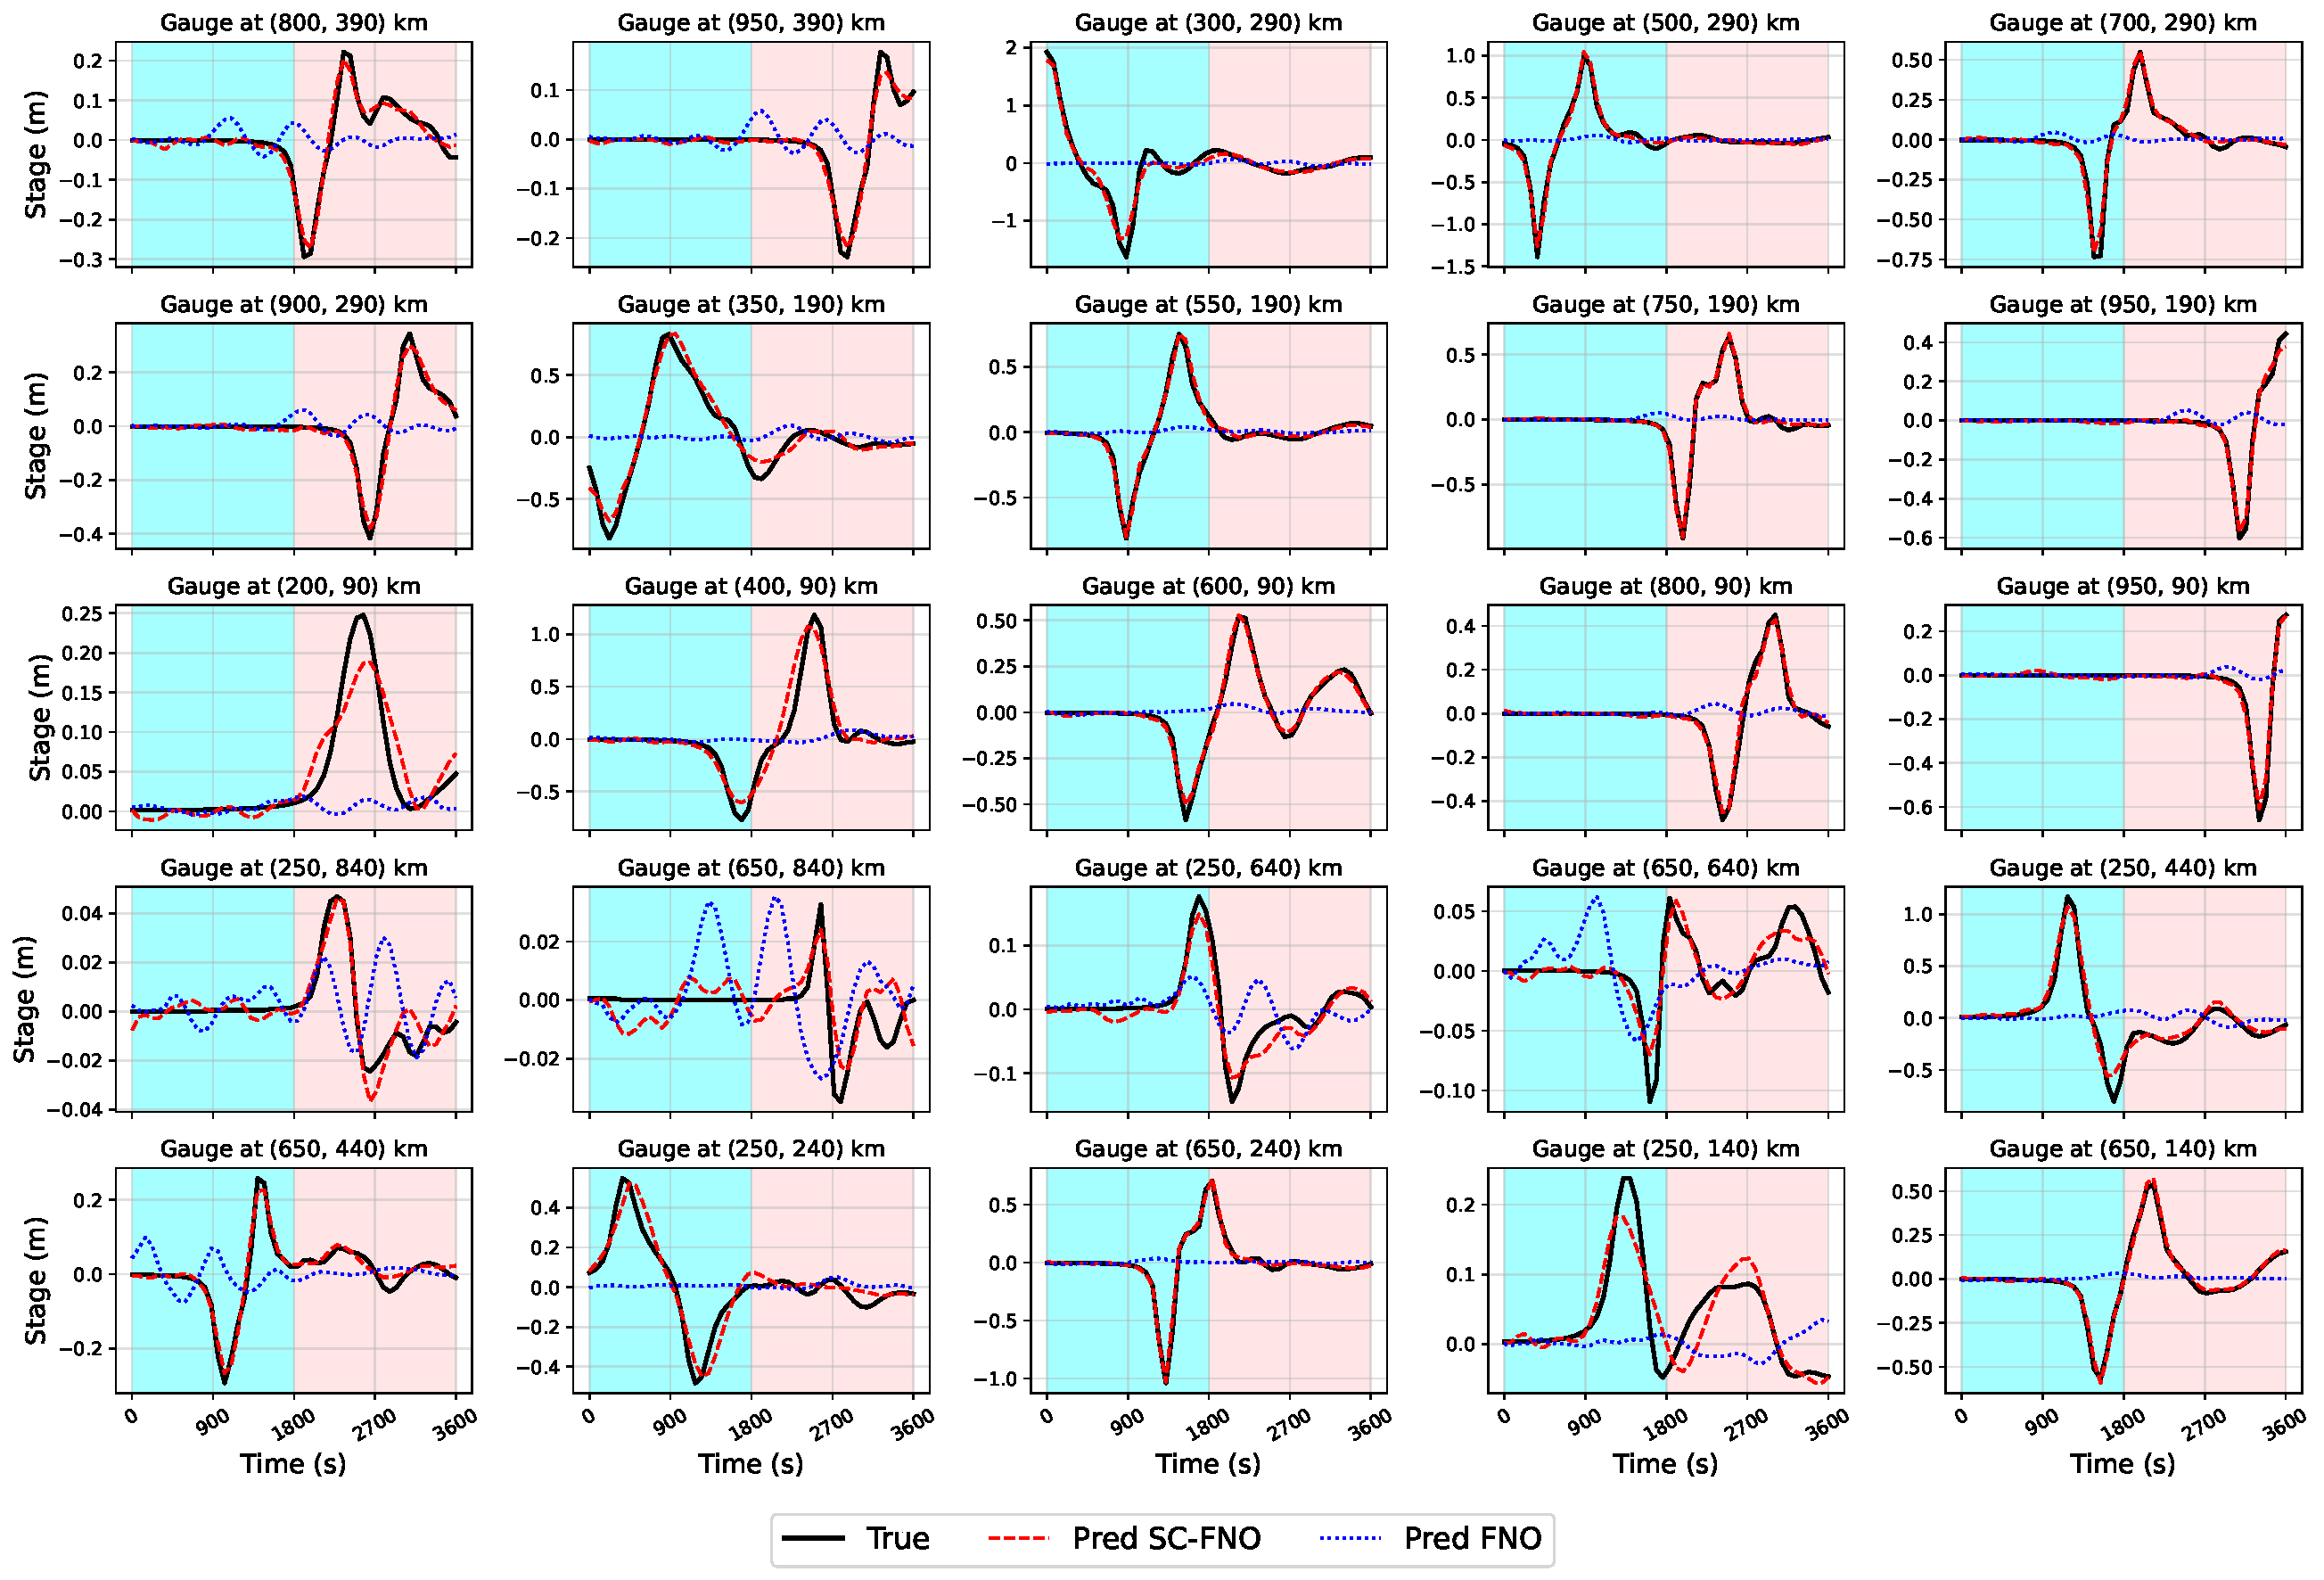
\includegraphics[width=0.98\textwidth, trim={0 0 0 0}, clip]{Figuers/PDE3_sensor_history.pdf}
\caption{\scriptsize\textbf{Reconstructed tsunami gauge time series using the inferred Okada deformation.} Comparison between observed (black), SC-FNO predictions (red dashed), and FNO predictions (blue dotted) at multiple gauge locations. The aqua-shaded regions denote the early portion of the event ($T_u = 30$,min) used as input for inversion, while the light-red regions represent the unseen time window predicted by the models.
}
\label{fig:gauge_timeseries}
\end{figure}




\subsection*{Additional results for PDE3}

% Table for performances of models for forward prediction of PDE3 
\begin{table}[htbp]
\centering
\caption{\scriptsize\textbf{Comparison of Error Metrics Across Models Trained with Different Sample Sizes (in-training) PDE3}}
\label{tab:pde3_forward_nostd}
\scriptsize
\setlength{\tabcolsep}{3pt}
\begin{tabular}{lcccccccc}
\hline
\textbf{Model} & \multicolumn{2}{c}{\textbf{1200 Samples}} & \multicolumn{2}{c}{\textbf{1000 Samples}} & \multicolumn{2}{c}{\textbf{700 Samples}} & \multicolumn{2}{c}{\textbf{200 Samples}} \\
 & \textbf{Rel. \(L^2\)} & \textbf{MAE} & \textbf{Rel. \(L^2\)} & \textbf{MAE} & \textbf{Rel. \(L^2\)} & \textbf{MAE} & \textbf{Rel. \(L^2\)} & \textbf{MAE} \\
\hline
FNO        & \(7.1 \times 10^{-2}\) & \(6.8 \times 10^{-2}\) & \(8.9 \times 10^{-2}\) & \(7.6 \times 10^{-2}\) & \(1.12 \times 10^{-1}\) & \(9.2 \times 10^{-2}\) & \(5.9 \times 10^{-1}\) & \(5.8 \times 10^{-1}\) \\
WNO        & \(7.6 \times 10^{-2}\) & \(7.3 \times 10^{-2}\) & \(9.5 \times 10^{-2}\) & \(8.1 \times 10^{-2}\) & \(1.18 \times 10^{-1}\) & \(9.9 \times 10^{-2}\) & \(6.3 \times 10^{-1}\) & \(6.2 \times 10^{-1}\) \\
DeepONet   & \(8.2 \times 10^{-2}\) & \(7.9 \times 10^{-2}\) & \(1.01 \times 10^{-1}\) & \(8.7 \times 10^{-2}\) & \(1.25 \times 10^{-1}\) & \(1.0 \times 10^{-1}\) & \(6.7 \times 10^{-1}\) & \(6.7 \times 10^{-1}\) \\
SC-FNO     & \(\mathbf{1.1 \times 10^{-2}}\) & \(\mathbf{2.2 \times 10^{-2}}\) & \(\mathbf{2.8 \times 10^{-2}}\) & \(\mathbf{5.6 \times 10^{-2}}\) & \(\mathbf{6.2 \times 10^{-2}}\) & \(\mathbf{1.0 \times 10^{-1}}\) & \(\mathbf{1.3 \times 10^{-1}}\) & \(\mathbf{2.3 \times 10^{-1}}\) \\
SC-WNO     & \(1.2 \times 10^{-2}\) & \(2.4 \times 10^{-2}\) & \(3.0 \times 10^{-2}\) & \(5.9 \times 10^{-2}\) & \(6.5 \times 10^{-2}\) & \(1.1 \times 10^{-1}\) & \(1.4 \times 10^{-1}\) & \(2.5 \times 10^{-1}\) \\
SC-DeepONet& \(1.5 \times 10^{-2}\) & \(2.8 \times 10^{-2}\) & \(3.6 \times 10^{-2}\) & \(7.0 \times 10^{-2}\) & \(7.1 \times 10^{-2}\) & \(1.2 \times 10^{-1}\) & \(1.6 \times 10^{-1}\) & \(2.9 \times 10^{-1}\) \\
\hline
\end{tabular}
\end{table}

% Table for performances of models for forward prediction of PDE3 (out-of-training / OOD)
\begin{table}[htbp]
\centering
\caption{\scriptsize\textbf{Comparison of Error Metrics Across Models Trained with Different Sample Sizes (out-of-training) PDE3}}
\label{tab:pde3_forward_ood}
\scriptsize
\setlength{\tabcolsep}{3pt}
\begin{tabular}{lcccccccc}
\hline
\textbf{Model} & \multicolumn{2}{c}{\textbf{1200 Samples}} & \multicolumn{2}{c}{\textbf{1000 Samples}} & \multicolumn{2}{c}{\textbf{700 Samples}} & \multicolumn{2}{c}{\textbf{200 Samples}} \\
 & \textbf{Rel. \(L^2\)} & \textbf{MAE} & \textbf{Rel. \(L^2\)} & \textbf{MAE} & \textbf{Rel. \(L^2\)} & \textbf{MAE} & \textbf{Rel. \(L^2\)} & \textbf{MAE} \\
\hline
FNO        & \(1.3 \times 10^{-1}\) & \(1.1 \times 10^{-1}\) & \(1.6 \times 10^{-1}\) & \(1.3 \times 10^{-1}\) & \(1.9 \times 10^{-1}\) & \(1.6 \times 10^{-1}\) & \(7.5 \times 10^{-1}\) & \(6.5 \times 10^{-1}\) \\
WNO        & \(1.4 \times 10^{-1}\) & \(1.2 \times 10^{-1}\) & \(1.8 \times 10^{-1}\) & \(1.4 \times 10^{-1}\) & \(2.1 \times 10^{-1}\) & \(1.7 \times 10^{-1}\) & \(8.0 \times 10^{-1}\) & \(6.9 \times 10^{-1}\) \\
DeepONet   & \(1.5 \times 10^{-1}\) & \(1.3 \times 10^{-1}\) & \(1.9 \times 10^{-1}\) & \(1.5 \times 10^{-1}\) & \(2.3 \times 10^{-1}\) & \(1.9 \times 10^{-1}\) & \(8.5 \times 10^{-1}\) & \(7.2 \times 10^{-1}\) \\
SC-FNO     & \(\mathbf{3.5 \times 10^{-2}}\) & \(\mathbf{6.0 \times 10^{-2}}\) & \(\mathbf{5.0 \times 10^{-2}}\) & \(\mathbf{8.0 \times 10^{-2}}\) & \(\mathbf{8.0 \times 10^{-2}}\) & \(\mathbf{1.0 \times 10^{-1}}\) & \(\mathbf{2.5 \times 10^{-1}}\) & \(\mathbf{3.0 \times 10^{-1}}\) \\
SC-WNO     & \(3.8 \times 10^{-2}\) & \(6.5 \times 10^{-2}\) & \(5.3 \times 10^{-2}\) & \(8.5 \times 10^{-2}\) & \(8.5 \times 10^{-2}\) & \(1.1 \times 10^{-1}\) & \(2.7 \times 10^{-1}\) & \(3.2 \times 10^{-1}\) \\
SC-DeepONet& \(4.2 \times 10^{-2}\) & \(7.0 \times 10^{-2}\) & \(5.7 \times 10^{-2}\) & \(9.0 \times 10^{-2}\) & \(9.5 \times 10^{-2}\) & \(1.2 \times 10^{-1}\) & \(3.0 \times 10^{-1}\) & \(3.5 \times 10^{-1}\) \\
\hline
\end{tabular}
\end{table}




% % \clearpage
% % 
% \section*{Theoretical Justification for Sensitivity-Constrained Training} \label{prove}

% We provide a mathematical basis for why Sensitivity-Constrained Neural Operators (SC-NOs) outperform standard training by incorporating sensitivity loss, improving generalization, long-term stability, and inversion accuracy.

% We define the operator $\mathcal{G}_\theta: \mathcal{U} \to \mathcal{V}$, which maps an input function $a(x) = (u_0(x), p(x))$ to $\hat{u}(x,t) = \mathcal{G}_\theta(a(x))$, approximating the true solution $u(x,t)$.

% \subsubsection*{Assumptions and Notation}

% We work in bounded domains: the parameter space $\mathcal{P}_{\text{param}} \subset \mathbb{R}^m$ and the spatio-temporal domain $\mathcal{X} \times [0,T]$. We assume $\hat{u}$ is differentiable with respect to $p$. We use the Euclidean norm $|\cdot|$ on $\mathbb{R}^m$ and the corresponding induced operator norms.

% We assume the true solution $u$ and its sensitivity $\frac{\partial u}{\partial p}$ are bounded by $M$ and $M_p$ respectively, for all $(x,t,p)$.
% \begin{equation}
% |u(x,t;p)| \leq M, \quad \left\| \frac{\partial u}{\partial p}(x,t;p) \right\| \leq M_p.
% \end{equation}

% Our core argument relies on standard (though strong) assumptions from learning theory: for an overparameterized, well-trained model $\theta_s^*$, a small empirical loss implies a small uniform error bound.

% \textbf{Assumption 1 (Uniform Convergence of Gradients):}
% We assume that a model $\theta_s^*$ trained to $L_s(\theta_s^*)$ on $n$ samples satisfies:
% \begin{equation}
% \sup_{x,t,p} \left\| \frac{\partial \hat{u}}{\partial p}(x,t;p;\theta_s^*) - \frac{\partial u}{\partial p}(x,t;p) \right\| \le \varepsilon_s
% \end{equation}
% where $\varepsilon_s \to 0$ as $L_s \to 0$ and $n \to \infty$.

% \textbf{Assumption 2 (Uniform Convergence of Solutions):}
% We assume a similar uniform bound $\varepsilon_u$ for the solution itself:
% \begin{equation}
% \sup_{x,t,p} |\hat{u}(x,t;p;\theta_s^*) - u(x,t;p)| \le \varepsilon_u
% \end{equation}
% where $\varepsilon_u \to 0$ as $L_u \to 0$ and $n \to \infty$.

% \subsubsection*{Cost Functionals}

% Training minimizes the following losses, where $\frac{\partial u}{\partial p}$ is computed on-the-fly via a differentiable solver or adjoint model:
% \begin{equation}
% L_u(\theta) = \frac{1}{n} \sum_{i=1}^n [\hat{u}(x_i, t_i; p_i;\theta) - u(x_i, t_i; p_i)]^2,
% \end{equation}
% \begin{equation}
% L_s(\theta) = \frac{1}{n} \sum_{i=1}^n \left\| \frac{\partial \hat{u}}{\partial p}(x_i, t_i; p_i;\theta) - \frac{\partial u}{\partial p}(x_i, t_i; p_i) \right\|^2,
% \end{equation}
% \begin{equation}
% L(\theta) = L_u(\theta) + \lambda L_s(\theta), \quad \lambda > 0.
% \end{equation}


% \subsubsection*{Improved Generalization}

% Training with $L(\theta)$ acts as a powerful regularizer by explicitly constraining the model's Lipschitz constant with respect to parameters. We define this constant as:
% \begin{equation}
% L_{\text{lip}}(\theta) = \sup_{x,t,p} \left\| \frac{\partial \hat{u}}{\partial p}(x,t;p;\theta) \right\|.
% \end{equation}
% For the sensitivity-constrained model $\theta_s^*$, we can rigorously bound its Lipschitz constant using Assumption 1 and the triangle inequality:
% \begin{align}
% L_{\text{lip}}(\theta_s^*) &= \sup \left\| \frac{\partial u}{\partial p} + \left( \frac{\partial \hat{u}}{\partial p} - \frac{\partial u}{\partial p} \right) \right\| \notag \\
% &\le \sup \left\| \frac{\partial u}{\partial p} \right\| + \sup \left\| \frac{\partial \hat{u}}{\partial p} - \frac{\partial u}{\partial p} \right\| \notag \\
% &\le M_p + \varepsilon_s.
% \end{align}
% By driving $\varepsilon_s \to 0$, we force the model to inherit the (bounded) Lipschitz constant of the true physical system.

% This has a direct impact on generalization. For fixed $(x,t)$, we define the hypothesis class $\mathcal{F}_{\text{SC}} = \{p \mapsto \hat{u}(x,t;p;\theta): L_{\text{lip}}(\theta) \le M_p+\varepsilon_s\}$. On a bounded parameter domain, standard results imply that the empirical Rademacher complexity $\hat{R}_n(\mathcal{F}_{\text{SC}})$ of this class scales linearly with its Lipschitz constant, $\hat{R}_n(\mathcal{F}_{\text{SC}}) \lesssim (M_p + \varepsilon_s)$. This complexity is strictly lower than that of an unconstrained class $\mathcal{F}_u$ that admits arbitrarily large Lipschitz constants. The standard generalization bound,
% \begin{equation}
% \mathbb{E}[(\hat{u} - u)^2] \leq L_u(\theta) + 2 \hat{R}_n(\mathcal{F}) + \text{ComplexityPenalty}(\delta, n),
% \end{equation}
% is therefore tighter for $\mathcal{F}_{\text{SC}}$, implying better performance on unseen parameters.


% \subsubsection*{Long-Term Prediction Stability}

% This argument is most clearly made by setting the parameter $p$ to be the initial condition $u_0$. The sensitivity $\frac{\partial u(t)}{\partial u_0}$ is the \textbf{fundamental solution operator}, and its norm governs the growth of perturbations (i.e., the Lyapunov exponents).

% Assume the true physical system's growth is bounded:
% \begin{equation}
% \left\| \frac{\partial u(t)}{\partial u_0} \right\| \le C e^{\alpha t}
% \end{equation}
% for some physical exponent $\alpha$ (which could be positive for a chaotic system, or negative for a stable one).

% A standard model $\theta_u^*$, trained only on $L_u$, may learn an incorrect operator $\frac{\partial \hat{u}}{\partial u_0}$ with a much larger exponent $\hat{\alpha} \gg \alpha$, leading to spurious amplification of small errors.

% The SC-NO, by minimizing $L_s$ (with $p=u_0$), uses Assumption 1 to force its learned operator to be close to the true one:
% \begin{align}
% \left\| \frac{\partial \hat{u}(t)}{\partial u_0} \right\| &\le \left\| \frac{\partial u(t)}{\partial u_0} \right\| + \sup \left\| \frac{\partial \hat{u}}{\partial u_0} - \frac{\partial u}{\partial u_0} \right\| \notag \\
% &\le C e^{\alpha t} + \varepsilon_s.
% \end{align}
% This shows that the SC-NO reproduces the physical growth rates of perturbations up to $O(\varepsilon_s)$ and does not introduce spurious instabilities beyond those present in the governing system.


% \subsubsection*{Inversion Accuracy}

% In parameter inversion, we seek to find $p^*$ by minimizing a loss $\ell$ between our model $\hat{u}$ and an observation $u_{\text{obs}}$. Let $J(p) = \ell(u(p), u_{\text{obs}})$ be the "true" (but intractable) loss landscape, and $J_\theta(p) = \ell(\hat{u}_\theta(p), u_{\text{obs}})$ be the surrogate landscape our optimizer actually sees.

% Gradient descent updates use the gradient of $J_\theta$:
% \begin{equation}
% p_{k+1} = p_k - \eta \nabla_p J_\theta(p_k), \quad \text{where} \quad \nabla_p J_\theta = \frac{\partial \ell}{\partial \hat{u}} \cdot \frac{\partial \hat{u}}{\partial p}.
% \end{equation}
% The success of the inversion depends on the \textbf{gradient error} $\|\nabla J_\theta(p) - \nabla J(p)\|$. If $\ell$ is smooth, this error is bounded by our assumed uniform errors:
% \begin{equation}
% \|\nabla J_\theta(p) - \nabla J(p)\| \le C_1 \varepsilon_u + C_2 \varepsilon_s
% \end{equation}
% for some constants $C_1, C_2$.

% A standard model $\theta_u^*$ is only trained to minimize $\varepsilon_u$, leaving a large, uncontrolled gradient error $C_2 \varepsilon_s$. The optimizer is fed an inaccurate gradient. An SC-NO is explicitly trained to drive both $\varepsilon_u \to 0$ and $\varepsilon_s \to 0$. We further assume that, in a neighborhood of $p^*$, the true objective $J(p)$ is $\mu$-strongly convex. Under this condition, standard perturbation results for gradient descent imply that optimization on $J_\theta$ converges to an $O(\varepsilon_u + \varepsilon_s)$ neighborhood of the true optimum $p^*$. By minimizing $\varepsilon_s$, SC-NOs guarantee a high-fidelity gradient, ensuring a much more accurate and stable convergence.


















% \section*{Theoretical Justification for Sensitivity-Constrained Training} \label{prove}

% We provide a mathematical basis for why Sensitivity-Constrained Neural Operators (SC-NOs) outperform standard training by incorporating sensitivity loss, improving generalization, long-term stability, and inversion accuracy.

% We define the operator \(\mathcal{G}_\theta: \mathcal{U} \to \mathcal{V}\), which maps \( a(x) = (u_0(x), p(x)) \) to \(\hat{u}(x,t) = \mathcal{G}_\theta(a(x))\), approximating the true solution \( u(x,t) \). Both are continuously differentiable with respect to \( p \in \mathbb{R}^m \) over a bounded domain \(\mathcal{X} \times [0,T]\). The dataset consists of i.i.d. samples 

% \begin{equation}
% D = \{ (x_i, t_i, p_i, u(x_i, t_i; p_i), \frac{\partial u}{\partial p}(x_i, t_i; p_i)) \}_{i=1}^n
% \end{equation}

% drawn from a distribution \(\mathcal{P}\) over \(\mathcal{X} \times [0,T] \times \mathcal{P}_{\text{param}}\), where \(\mathcal{P}_{\text{param}}\) is a bounded subset of \(\mathbb{R}^m\) with \( \|p\| \leq P_{\text{max}} \). 

% The function outputs are bounded, with constants \( M, M_p > 0 \) satisfying

% \begin{equation}
% |\hat{u}(x,t;p;\theta)|, |u(x,t;p)| \leq M, \quad \left\| \frac{\partial \hat{u}}{\partial p}(x,t;p;\theta) \right\|, \left\| \frac{\partial u}{\partial p}(x,t;p) \right\| \leq M_p.
% \end{equation}

% The optimization landscape is assumed to be well-posed, with practical optima \(\theta_u^*\) and \(\theta_s^*\) achieving near-global minima in \(\Theta\). Training minimizes the following losses:

% \begin{equation}
% L_u(\theta) = \frac{1}{n} \sum_{i=1}^n [\hat{u}(x_i, t_i; p_i;\theta) - u(x_i, t_i; p_i)]^2,
% \end{equation}

% \begin{equation}
% L_s(\theta) = \frac{1}{n} \sum_{i=1}^n \left\| \frac{\partial \hat{u}}{\partial p}(x_i, t_i; p_i;\theta) - \frac{\partial u}{\partial p}(x_i, t_i; p_i) \right\|^2,
% \end{equation}

% \begin{equation}
% L(\theta) = L_u(\theta) + \lambda L_s(\theta), \quad \lambda > 0.
% \end{equation}

% \subsubsection*{Improved Generalization}

% For sufficiently large \(\lambda\), training with \(L(\theta)\) reduces complexity and improves generalization compared to \(L_u(\theta)\) alone. The Lipschitz constant of the model with respect to \( p \) is defined as:

% \begin{equation}
% L_{\text{lip}}(\theta) = \sup_{x,t,p} \left\| \frac{\partial \hat{u}}{\partial p}(x,t;p;\theta) \right\|.
% \end{equation}

% For any \( p, q \in \mathcal{P}_{\text{param}} \),

% \begin{equation}
% |\hat{u}(x,t;p;\theta) - \hat{u}(x,t;q;\theta)| \leq L_{\text{lip}}(\theta) \|p - q\|.
% \end{equation}

% With sensitivity training,

% \begin{equation}
% L_{\text{lip}}(\theta_s^*) \leq M_p + \sqrt{n L_s(\theta_s^*)},
% \end{equation}

% which ensures \( L_{\text{lip}}(\theta_s^*) < L_{\text{lip}}(\theta_u^*) \) as \( \lambda \to \infty \). This reduction in complexity leads to a lower Rademacher complexity,

% \begin{equation}
% \hat{R}_n(\mathcal{F}) \leq 2 L_{\text{lip}}(\theta) D \sqrt{\frac{2 \ln(2)}{n}}.
% \end{equation}

% Thus, the generalization bound

% \begin{equation}
% \mathbb{E}[(\hat{u} - u)^2] \leq L_u(\theta) + 2 \hat{R}_n(\mathcal{F}) + 3 \sqrt{\frac{\ln(2/\delta)}{2n}}
% \end{equation}

% is tighter for sensitivity-trained models, improving overall generalization.

% \subsubsection*{Long-Term Prediction Stability}

% Training with \( L(\theta) \) reduces error accumulation over time in dynamical systems. Defining the prediction error,

% \begin{equation}
% e(x,t;p;\theta) = \hat{u}(x,t;p;\theta) - u(x,t;p),
% \end{equation}

% the error growth is bounded by

% \begin{equation}
% |e(x,t;p;\theta)| \leq \int_0^t \left\| \frac{\partial \hat{u}}{\partial p}(x,s;p;\theta) - \frac{\partial u}{\partial p}(x,s;p) \right\| \|p\| \, ds.
% \end{equation}

% With probability \( 1 - \delta \),

% \begin{equation}
% \left\| \frac{\partial \hat{u}}{\partial p}(x,s;p;\theta_s^*) - \frac{\partial u}{\partial p}(x,s;p) \right\| \leq \sqrt{\frac{n L_s(\theta_s^*)}{\delta}},
% \end{equation}

% leading to

% \begin{equation}
% |e(x,t;p;\theta_s^*)| \leq t \sqrt{\frac{n L_s(\theta_s^*)}{\delta}} P_{\text{max}}.
% \end{equation}

% Since \( L_s(\theta_s^*) \to 0 \) as \( \lambda \to \infty \), sensitivity training mitigates long-term prediction errors.

% \subsubsection*{Inversion Accuracy}

% In parameter inversion, the goal is to solve

% \begin{equation}
% p^* = \arg\min_p \ell(\hat{u}(x,t;p;\theta), u_{\text{obs}}).
% \end{equation}

% Gradient updates follow

% \begin{equation}
% p_{k+1} = p_k - \eta \nabla_p \ell(p_k), \quad \nabla_p \ell = \frac{\partial \ell}{\partial \hat{u}} \cdot \frac{\partial \hat{u}}{\partial p}.
% \end{equation}

% For sensitivity-trained models, with probability \( 1 - \delta \),

% \begin{equation}
% \left\| \frac{\partial \hat{u}}{\partial p}(x,t;p;\theta_s^*) - \frac{\partial u}{\partial p}(x,t;p) \right\| \leq \sqrt{\frac{n L_s(\theta_s^*)}{\delta}},
% \end{equation}

% which ensures more accurate gradients and improved parameter recovery.\\
% We have demonstrated that training with \( L(\theta) = L_u(\theta) + \lambda L_s(\theta) \) provides key advantages. By constraining the Lipschitz constant, SC-NOs reduce complexity and achieve tighter generalization bounds. Minimizing sensitivity error stabilizes long-term predictions, and enforcing accurate gradients enhances parameter inversion. These results validate the effectiveness of SC-NOs in learning physically consistent representations, reinforcing their advantages over standard Neural Operators.



% % \clearpage
% % \section{Applicability, Limitations, and Future Extensions}

\renewcommand{\thefigure}{F.\arabic{figure}}  % Number figures as A.1, A.2, ...
\renewcommand{\thetable}{f.\arabic{table}}  % Number tables as A.1, A.2, ...


Sensitivity-constrained training requires Jacobians. This can be challenging in systems where adjoints are difficult to implement, unstable, infeasible, or prohibitively expensive, for example, highly chaotic or turbulent dynamics, nonlinear elastodynamics, or other mathematical non-differentiabilities. In such settings, operational systems may rely on large-scale ensembles or extreme-scale offline computation to retain full physical fidelity. Nevertheless, even in chaotic and turbulent systems, adjoint sensitivities are used operationally over the finite time windows in which they remain stable, as in 4D-Var and ensemble-variational data assimilation. SC-NO can therefore be applicable to a broad class of PDE-governed systems with locally stable adjoints.

While our SC-NO tsunami workflow is robust in the face of inversion uncertainty and moderate buoy data noise, it is not intended as an operational forecasting system, which must also account for additional uncertainties in rupture geometry, background currents, non-seismic sources, sensor outages, and near-coast inundation physics \citep{grezio2017probabilistic}. Future work can also incorporate seismic and sea floor sensor data to improve lead time. Rather than proposing a full operational paradigm, our current aim is to isolate a complementary computational contribution: real-time surrogate evaluation and minute-scale inversion. The method can, in principle, enable faster exploration of such uncertainties and facilitate data assimilation, particularly in settings where repeated full-physics solves would be prohibitive, although it does not replace existing operational pipelines. 

Prior studies have shown that a method that incorporates PDE equation loss like PINO can provide moderate improvements for state accuracy but does not directly constrain parameter sensitivities and introduces additional computational cost \citep{behroozi2025sensitivity} and future work can test its cost and benefit. Because our focus is on full-field, high-resolution surrogates that remain accurate under localized input perturbations and enable stable inversion, we did not compare against traditional reduced-order approaches such as Proper Orthogonal Decomposition, which are most effective when low-dimensional manifolds exist, nor against physics-informed neural networks (PINNs), which target different objectives such as knowledge discovery. Dimensionality-reduction and gradient-aware methods such as DINO or DE-DeepONet address complementary challenges—primarily representational efficiency—whereas SC-NO targets sensitivity, fidelity, and inverse stability. These approaches are orthogonal in design and span different axes of the accuracy–cost–conditioning trade space, and assessing whether low-dimensional representations preserve the reverse-scaling behavior identified here remains an important direction for future work.

Future directions include adaptive constraint weighting, higher-order (Hessian) supervision, uncertainty quantification via learned Jacobians, and adaptive search for optimal Jacobian sampling strategies. Collectively, these results position sensitivity-constrained training as a foundational enhancement to neural operators, enabling physically trustworthy surrogates for prediction, inversion, and decision-making under uncertainty.



% % \clearpage
% % \section{Performance Metrics}

To evaluate the performance of our neural operator models, we report two complementary metrics: the relative \( L^2 \) error and the mean absolute error (MAE). The relative \( L^2 \) error quantifies the normalized discrepancy between predicted and ground truth solutions, while the MAE captures average absolute deviations. This dual-metric approach ensures robustness by balancing scale-invariant accuracy (via \( L^2 \)) with direct magnitude sensitivity (via MAE). Specifically, we define:

\begin{equation}
\text{Relative } L^2 \text{ Error} := \frac{1}{N} \sum_{i=1}^{N} 
\frac{\left\| \mathcal{G}_\theta(a^{(i)}) - u^{(i)} \right\|_2}{\left\| u^{(i)} \right\|_2},
\end{equation}

\begin{equation}
\text{Mean Absolute Error (MAE)} := \frac{1}{N} \sum_{i=1}^{N} 
\left\| \mathcal{G}_\theta(a^{(i)}) - u^{(i)} \right\|_1,
\end{equation}

where \( N \) is the number of test samples, \( \mathcal{G}_\theta(a^{(i)}) \) is the model prediction for input \( a^{(i)} \), and \( u^{(i)} \) is the corresponding ground truth solution. Both metrics are computed over the full spatial-temporal domain of the PDE solutions.





% % \clearpage
% % \section{Experiments}
\label{sec:EXP}

\renewcommand{\thefigure}{G.\arabic{figure}}  % Number figures as A.1, A.2, ...
\renewcommand{\thetable}{G.\arabic{table}}  % Number tables as A.1, A.2, ...

To evaluate the performance of Neural Operators (NOs) and Sensitivity-Constrained Neural Operators (SC-NOs), we design two primary classes of experiments based on the direction of inference with respect to the solution operator \( \mathcal{G}_\theta \):


\subsection*{Forward Prediction}

In this setting, the objective is to train a model to predict the future states of the system \( u(\mathbf{x}, t, p) \) given partial temporal information and the spatial parameter field. The model learns the forward mapping:
\begin{equation}
\mathcal{G}_\theta: a(\mathbf{x}, t, p) \mapsto u(\mathbf{x}, t, p),
\end{equation}
where the input \( a(\mathbf{x}, t, p) = \big(a_{\text{init}}(\mathbf{x}, t),\; p(\mathbf{x})\big) \) includes the first \( t_u \) time steps of the solution and the spatially varying parameters \( p(\mathbf{x}) \). The model is trained to generate the solution over the remaining time interval \( [t_u, T] \), and performance is measured using metrics such as relative \( L^2 \) error and mean absolute error (MAE).

\subsection*{Inverse Inference via Optimization}

In the second class of experiments, we treat the trained NO or SC-NO as a differentiable surrogate and use it in a gradient-based optimization loop to recover the unknown input function \( a(\mathbf{x}, t, p) \), particularly the parameter field \( p(\mathbf{x}) \), from a given solution trajectory \( u(\mathbf{x}, t, p) \). This inverse inference is formalized as:
\begin{equation}
\min_{a(\mathbf{x}, t, p)} \| \mathcal{G}_\theta(a) - u_{\text{target}}(\mathbf{x}, t) \|^2,
\end{equation}
where \( u_{\text{target}}(\mathbf{x}, t) \) is the observed or target solution path. The optimization leverages automatic differentiation through \( \mathcal{G}_\theta \), and the accuracy of the inferred parameters is evaluated by comparing the recovered \( p(\mathbf{x}) \) to ground truth.

\vspace{6pt}
Together, these two types of experiments provide a comprehensive evaluation of both predictive accuracy and gradient quality, allowing us to assess the effectiveness of sensitivity constraints in improving model generalization and interpretability.


% % \clearpage
% % \section{Hyperparameters and Settings}
\renewcommand{\thefigure}{H.\arabic{figure}}  % Number figures as A.1, A.2, ...
\renewcommand{\thetable}{H.\arabic{table}}  % Number tables as A.1, A.2, ...

All models were trained using the Adam optimizer with a batch size of 16, an initial learning rate of 0.001, a learning rate scheduler with a decay factor $\gamma = 0.95$ applied every 100 epochs. The training was conducted over a spatiotemporal domain discretized into a $n_x \times n_y$ spatial grid. The total number of time steps $n_t$ is given by $n_t = t_u + t_G$, where $t_u$ is the number of input time steps and $t_G$ is the number of predicted time steps. Model-specific hyperparameters are summarized in the tables below.


\begin{table}[htbp]
\centering
\scriptsize
\setlength{\tabcolsep}{4pt}
\begin{minipage}[t]{0.48\textwidth}
\centering
\caption{\scriptsize\textbf{FNO hyper-parameters for all PDEs}}
\label{tab:fno_hparams}
\begin{tabular}{lccc}
\hline
\textbf{Parameter} & \textbf{PDE1} & \textbf{PDE2} & \textbf{PDE3} \\
\hline
Fourier modes $(x, y, t)$ & (8, 8, 8) & (8, 8, 8) & (8, 8, 8) \\
Width & 20 & 20 & 20 \\
Training epochs & 500 & 500 & 1000\\
$n_x$ & 50& 64& 100\\
$n_y$ & 50& 64& 100\\
$t_u$ & 1& 1& 1\\
$t_G$ & 99& 29& 50\\
$n_t$ & 100& 30& 51\\
\hline
\end{tabular}
\end{minipage}%
\hfill
\begin{minipage}[t]{0.48\textwidth}
\centering
\caption{\scriptsize\textbf{WNO hyper-parameters for all PDEs}}
\label{tab:wno_hparams}
\begin{tabular}{lccc}
\hline
\textbf{Parameter} & \textbf{PDE1} & \textbf{PDE2} & \textbf{PDE3} \\
\hline
Wavelet basis & db6 & db6 & db6 \\
Decomposition level & 4 & 4 & 4 \\
Width & 30 & 30 & 30 \\
Number of wavelet layers & 4 & 4 & 4 \\
Training epochs & 500 & 500 & 1000\\
$n_x$ & 50& 64& 100\\
$n_y$ & 50& 64& 100\\
$t_u$ & 1& 1& 1\\
$t_G$ & 99& 29& 50\\
$n_t$ & 100& 30& 51\\
\hline
\end{tabular}
\end{minipage}
\end{table}



\begin{table}[htbp]
\centering
\caption{\scriptsize\textbf{DeepONet hyper-parameters for all PDEs}}
\label{tab:deeponet_hparams}
\scriptsize
\setlength{\tabcolsep}{5pt}
\begin{tabular}{lccc}
\hline
\textbf{Parameter} & \textbf{PDE1} & \textbf{PDE2} & \textbf{PDE3} \\
\hline
Branch network layers & [64, 128, 128, 128, 64] & [64, 128, 128, 128, 64] & [64, 128, 128, 128, 64] \\
Trunk network layers & [64, 128, 128, 128, 64] & [64, 128, 128, 128, 64] & [64, 128, 128, 128, 64] \\
Training epochs & 500 & 500 & 1000\\
$n_x$ & 50& 64& 100\\
$n_y$ & 50& 64& 100\\
$t_u$ &  1&  1&  1\\
$t_G$ &  99&  29&  50\\
$n_t$ & 100& 30& 51\\
\hline
\end{tabular}
\end{table}












% \begin{table}[htbp]
% \centering
% \caption{\textbf{FNO hyper-parameters for all PDEs}}
% \label{tab:fno_hparams}
% \scriptsize
% \setlength{\tabcolsep}{5pt}
% \begin{tabular}{lccc}
% \hline
% \textbf{Parameter} & \textbf{PDE1} & \textbf{PDE2} & \textbf{PDE3} \\
% \hline
% Fourier modes $(x, y, t)$ & (8, 8, 8) & (8, 8, 8) & (8, 8, 8) \\
% Width & 20 & 20 & 20 \\
% Training epochs & 500 & 500 & 1000\\
% $n_x$ & 50& 64& 100\\
% $n_y$ & 50& 64& 100\\
% $t_u$ &  1&  1&  1\\
% $t_G$ &  99&  29&  50\\
% $n_t$ & 100& 30& 51\\
% \hline
% \end{tabular}
% \end{table}

% \vspace{1em}

% \begin{table}[htbp]
% \centering
% \caption{\textbf{WNO hyper-parameters for all PDEs}}
% \label{tab:wno_hparams}
% \scriptsize
% \setlength{\tabcolsep}{5pt}
% \begin{tabular}{lccc}
% \hline
% \textbf{Parameter} & \textbf{PDE1} & \textbf{PDE2} & \textbf{PDE3} \\
% \hline
% Wavelet basis & db6 & db6 & db6 \\
% Decomposition level & 4 & 4 & 4 \\
% Width & 30 & 30 & 30 \\
% Number of wavelet layers & 4 & 4 & 4 \\
% Training epochs & 500 & 500 & 1000\\
% $n_x$ & 50& 64& 100\\
% $n_y$ & 50& 64& 100\\
% $t_u$ &  1&  1&  1\\
% $t_G$ &  99&  29&  50\\
% $n_t$ & 100& 30& 51\\
% \hline
% \end{tabular}
% \end{table}

% % % \clearpage
% % % 
% \section*{Theoretical Justification for Sensitivity-Constrained Training} \label{prove}

% We provide a mathematical basis for why Sensitivity-Constrained Neural Operators (SC-NOs) outperform standard training by incorporating sensitivity loss, improving generalization, long-term stability, and inversion accuracy.

% We define the operator $\mathcal{G}_\theta: \mathcal{U} \to \mathcal{V}$, which maps an input function $a(x) = (u_0(x), p(x))$ to $\hat{u}(x,t) = \mathcal{G}_\theta(a(x))$, approximating the true solution $u(x,t)$.

% \subsubsection*{Assumptions and Notation}

% We work in bounded domains: the parameter space $\mathcal{P}_{\text{param}} \subset \mathbb{R}^m$ and the spatio-temporal domain $\mathcal{X} \times [0,T]$. We assume $\hat{u}$ is differentiable with respect to $p$. We use the Euclidean norm $|\cdot|$ on $\mathbb{R}^m$ and the corresponding induced operator norms.

% We assume the true solution $u$ and its sensitivity $\frac{\partial u}{\partial p}$ are bounded by $M$ and $M_p$ respectively, for all $(x,t,p)$.
% \begin{equation}
% |u(x,t;p)| \leq M, \quad \left\| \frac{\partial u}{\partial p}(x,t;p) \right\| \leq M_p.
% \end{equation}

% Our core argument relies on standard (though strong) assumptions from learning theory: for an overparameterized, well-trained model $\theta_s^*$, a small empirical loss implies a small uniform error bound.

% \textbf{Assumption 1 (Uniform Convergence of Gradients):}
% We assume that a model $\theta_s^*$ trained to $L_s(\theta_s^*)$ on $n$ samples satisfies:
% \begin{equation}
% \sup_{x,t,p} \left\| \frac{\partial \hat{u}}{\partial p}(x,t;p;\theta_s^*) - \frac{\partial u}{\partial p}(x,t;p) \right\| \le \varepsilon_s
% \end{equation}
% where $\varepsilon_s \to 0$ as $L_s \to 0$ and $n \to \infty$.

% \textbf{Assumption 2 (Uniform Convergence of Solutions):}
% We assume a similar uniform bound $\varepsilon_u$ for the solution itself:
% \begin{equation}
% \sup_{x,t,p} |\hat{u}(x,t;p;\theta_s^*) - u(x,t;p)| \le \varepsilon_u
% \end{equation}
% where $\varepsilon_u \to 0$ as $L_u \to 0$ and $n \to \infty$.

% \subsubsection*{Cost Functionals}

% Training minimizes the following losses, where $\frac{\partial u}{\partial p}$ is computed on-the-fly via a differentiable solver or adjoint model:
% \begin{equation}
% L_u(\theta) = \frac{1}{n} \sum_{i=1}^n [\hat{u}(x_i, t_i; p_i;\theta) - u(x_i, t_i; p_i)]^2,
% \end{equation}
% \begin{equation}
% L_s(\theta) = \frac{1}{n} \sum_{i=1}^n \left\| \frac{\partial \hat{u}}{\partial p}(x_i, t_i; p_i;\theta) - \frac{\partial u}{\partial p}(x_i, t_i; p_i) \right\|^2,
% \end{equation}
% \begin{equation}
% L(\theta) = L_u(\theta) + \lambda L_s(\theta), \quad \lambda > 0.
% \end{equation}


% \subsubsection*{Improved Generalization}

% Training with $L(\theta)$ acts as a powerful regularizer by explicitly constraining the model's Lipschitz constant with respect to parameters. We define this constant as:
% \begin{equation}
% L_{\text{lip}}(\theta) = \sup_{x,t,p} \left\| \frac{\partial \hat{u}}{\partial p}(x,t;p;\theta) \right\|.
% \end{equation}
% For the sensitivity-constrained model $\theta_s^*$, we can rigorously bound its Lipschitz constant using Assumption 1 and the triangle inequality:
% \begin{align}
% L_{\text{lip}}(\theta_s^*) &= \sup \left\| \frac{\partial u}{\partial p} + \left( \frac{\partial \hat{u}}{\partial p} - \frac{\partial u}{\partial p} \right) \right\| \notag \\
% &\le \sup \left\| \frac{\partial u}{\partial p} \right\| + \sup \left\| \frac{\partial \hat{u}}{\partial p} - \frac{\partial u}{\partial p} \right\| \notag \\
% &\le M_p + \varepsilon_s.
% \end{align}
% By driving $\varepsilon_s \to 0$, we force the model to inherit the (bounded) Lipschitz constant of the true physical system.

% This has a direct impact on generalization. For fixed $(x,t)$, we define the hypothesis class $\mathcal{F}_{\text{SC}} = \{p \mapsto \hat{u}(x,t;p;\theta): L_{\text{lip}}(\theta) \le M_p+\varepsilon_s\}$. On a bounded parameter domain, standard results imply that the empirical Rademacher complexity $\hat{R}_n(\mathcal{F}_{\text{SC}})$ of this class scales linearly with its Lipschitz constant, $\hat{R}_n(\mathcal{F}_{\text{SC}}) \lesssim (M_p + \varepsilon_s)$. This complexity is strictly lower than that of an unconstrained class $\mathcal{F}_u$ that admits arbitrarily large Lipschitz constants. The standard generalization bound,
% \begin{equation}
% \mathbb{E}[(\hat{u} - u)^2] \leq L_u(\theta) + 2 \hat{R}_n(\mathcal{F}) + \text{ComplexityPenalty}(\delta, n),
% \end{equation}
% is therefore tighter for $\mathcal{F}_{\text{SC}}$, implying better performance on unseen parameters.


% \subsubsection*{Long-Term Prediction Stability}

% This argument is most clearly made by setting the parameter $p$ to be the initial condition $u_0$. The sensitivity $\frac{\partial u(t)}{\partial u_0}$ is the \textbf{fundamental solution operator}, and its norm governs the growth of perturbations (i.e., the Lyapunov exponents).

% Assume the true physical system's growth is bounded:
% \begin{equation}
% \left\| \frac{\partial u(t)}{\partial u_0} \right\| \le C e^{\alpha t}
% \end{equation}
% for some physical exponent $\alpha$ (which could be positive for a chaotic system, or negative for a stable one).

% A standard model $\theta_u^*$, trained only on $L_u$, may learn an incorrect operator $\frac{\partial \hat{u}}{\partial u_0}$ with a much larger exponent $\hat{\alpha} \gg \alpha$, leading to spurious amplification of small errors.

% The SC-NO, by minimizing $L_s$ (with $p=u_0$), uses Assumption 1 to force its learned operator to be close to the true one:
% \begin{align}
% \left\| \frac{\partial \hat{u}(t)}{\partial u_0} \right\| &\le \left\| \frac{\partial u(t)}{\partial u_0} \right\| + \sup \left\| \frac{\partial \hat{u}}{\partial u_0} - \frac{\partial u}{\partial u_0} \right\| \notag \\
% &\le C e^{\alpha t} + \varepsilon_s.
% \end{align}
% This shows that the SC-NO reproduces the physical growth rates of perturbations up to $O(\varepsilon_s)$ and does not introduce spurious instabilities beyond those present in the governing system.


% \subsubsection*{Inversion Accuracy}

% In parameter inversion, we seek to find $p^*$ by minimizing a loss $\ell$ between our model $\hat{u}$ and an observation $u_{\text{obs}}$. Let $J(p) = \ell(u(p), u_{\text{obs}})$ be the "true" (but intractable) loss landscape, and $J_\theta(p) = \ell(\hat{u}_\theta(p), u_{\text{obs}})$ be the surrogate landscape our optimizer actually sees.

% Gradient descent updates use the gradient of $J_\theta$:
% \begin{equation}
% p_{k+1} = p_k - \eta \nabla_p J_\theta(p_k), \quad \text{where} \quad \nabla_p J_\theta = \frac{\partial \ell}{\partial \hat{u}} \cdot \frac{\partial \hat{u}}{\partial p}.
% \end{equation}
% The success of the inversion depends on the \textbf{gradient error} $\|\nabla J_\theta(p) - \nabla J(p)\|$. If $\ell$ is smooth, this error is bounded by our assumed uniform errors:
% \begin{equation}
% \|\nabla J_\theta(p) - \nabla J(p)\| \le C_1 \varepsilon_u + C_2 \varepsilon_s
% \end{equation}
% for some constants $C_1, C_2$.

% A standard model $\theta_u^*$ is only trained to minimize $\varepsilon_u$, leaving a large, uncontrolled gradient error $C_2 \varepsilon_s$. The optimizer is fed an inaccurate gradient. An SC-NO is explicitly trained to drive both $\varepsilon_u \to 0$ and $\varepsilon_s \to 0$. We further assume that, in a neighborhood of $p^*$, the true objective $J(p)$ is $\mu$-strongly convex. Under this condition, standard perturbation results for gradient descent imply that optimization on $J_\theta$ converges to an $O(\varepsilon_u + \varepsilon_s)$ neighborhood of the true optimum $p^*$. By minimizing $\varepsilon_s$, SC-NOs guarantee a high-fidelity gradient, ensuring a much more accurate and stable convergence.


















% \section*{Theoretical Justification for Sensitivity-Constrained Training} \label{prove}

% We provide a mathematical basis for why Sensitivity-Constrained Neural Operators (SC-NOs) outperform standard training by incorporating sensitivity loss, improving generalization, long-term stability, and inversion accuracy.

% We define the operator \(\mathcal{G}_\theta: \mathcal{U} \to \mathcal{V}\), which maps \( a(x) = (u_0(x), p(x)) \) to \(\hat{u}(x,t) = \mathcal{G}_\theta(a(x))\), approximating the true solution \( u(x,t) \). Both are continuously differentiable with respect to \( p \in \mathbb{R}^m \) over a bounded domain \(\mathcal{X} \times [0,T]\). The dataset consists of i.i.d. samples 

% \begin{equation}
% D = \{ (x_i, t_i, p_i, u(x_i, t_i; p_i), \frac{\partial u}{\partial p}(x_i, t_i; p_i)) \}_{i=1}^n
% \end{equation}

% drawn from a distribution \(\mathcal{P}\) over \(\mathcal{X} \times [0,T] \times \mathcal{P}_{\text{param}}\), where \(\mathcal{P}_{\text{param}}\) is a bounded subset of \(\mathbb{R}^m\) with \( \|p\| \leq P_{\text{max}} \). 

% The function outputs are bounded, with constants \( M, M_p > 0 \) satisfying

% \begin{equation}
% |\hat{u}(x,t;p;\theta)|, |u(x,t;p)| \leq M, \quad \left\| \frac{\partial \hat{u}}{\partial p}(x,t;p;\theta) \right\|, \left\| \frac{\partial u}{\partial p}(x,t;p) \right\| \leq M_p.
% \end{equation}

% The optimization landscape is assumed to be well-posed, with practical optima \(\theta_u^*\) and \(\theta_s^*\) achieving near-global minima in \(\Theta\). Training minimizes the following losses:

% \begin{equation}
% L_u(\theta) = \frac{1}{n} \sum_{i=1}^n [\hat{u}(x_i, t_i; p_i;\theta) - u(x_i, t_i; p_i)]^2,
% \end{equation}

% \begin{equation}
% L_s(\theta) = \frac{1}{n} \sum_{i=1}^n \left\| \frac{\partial \hat{u}}{\partial p}(x_i, t_i; p_i;\theta) - \frac{\partial u}{\partial p}(x_i, t_i; p_i) \right\|^2,
% \end{equation}

% \begin{equation}
% L(\theta) = L_u(\theta) + \lambda L_s(\theta), \quad \lambda > 0.
% \end{equation}

% \subsubsection*{Improved Generalization}

% For sufficiently large \(\lambda\), training with \(L(\theta)\) reduces complexity and improves generalization compared to \(L_u(\theta)\) alone. The Lipschitz constant of the model with respect to \( p \) is defined as:

% \begin{equation}
% L_{\text{lip}}(\theta) = \sup_{x,t,p} \left\| \frac{\partial \hat{u}}{\partial p}(x,t;p;\theta) \right\|.
% \end{equation}

% For any \( p, q \in \mathcal{P}_{\text{param}} \),

% \begin{equation}
% |\hat{u}(x,t;p;\theta) - \hat{u}(x,t;q;\theta)| \leq L_{\text{lip}}(\theta) \|p - q\|.
% \end{equation}

% With sensitivity training,

% \begin{equation}
% L_{\text{lip}}(\theta_s^*) \leq M_p + \sqrt{n L_s(\theta_s^*)},
% \end{equation}

% which ensures \( L_{\text{lip}}(\theta_s^*) < L_{\text{lip}}(\theta_u^*) \) as \( \lambda \to \infty \). This reduction in complexity leads to a lower Rademacher complexity,

% \begin{equation}
% \hat{R}_n(\mathcal{F}) \leq 2 L_{\text{lip}}(\theta) D \sqrt{\frac{2 \ln(2)}{n}}.
% \end{equation}

% Thus, the generalization bound

% \begin{equation}
% \mathbb{E}[(\hat{u} - u)^2] \leq L_u(\theta) + 2 \hat{R}_n(\mathcal{F}) + 3 \sqrt{\frac{\ln(2/\delta)}{2n}}
% \end{equation}

% is tighter for sensitivity-trained models, improving overall generalization.

% \subsubsection*{Long-Term Prediction Stability}

% Training with \( L(\theta) \) reduces error accumulation over time in dynamical systems. Defining the prediction error,

% \begin{equation}
% e(x,t;p;\theta) = \hat{u}(x,t;p;\theta) - u(x,t;p),
% \end{equation}

% the error growth is bounded by

% \begin{equation}
% |e(x,t;p;\theta)| \leq \int_0^t \left\| \frac{\partial \hat{u}}{\partial p}(x,s;p;\theta) - \frac{\partial u}{\partial p}(x,s;p) \right\| \|p\| \, ds.
% \end{equation}

% With probability \( 1 - \delta \),

% \begin{equation}
% \left\| \frac{\partial \hat{u}}{\partial p}(x,s;p;\theta_s^*) - \frac{\partial u}{\partial p}(x,s;p) \right\| \leq \sqrt{\frac{n L_s(\theta_s^*)}{\delta}},
% \end{equation}

% leading to

% \begin{equation}
% |e(x,t;p;\theta_s^*)| \leq t \sqrt{\frac{n L_s(\theta_s^*)}{\delta}} P_{\text{max}}.
% \end{equation}

% Since \( L_s(\theta_s^*) \to 0 \) as \( \lambda \to \infty \), sensitivity training mitigates long-term prediction errors.

% \subsubsection*{Inversion Accuracy}

% In parameter inversion, the goal is to solve

% \begin{equation}
% p^* = \arg\min_p \ell(\hat{u}(x,t;p;\theta), u_{\text{obs}}).
% \end{equation}

% Gradient updates follow

% \begin{equation}
% p_{k+1} = p_k - \eta \nabla_p \ell(p_k), \quad \nabla_p \ell = \frac{\partial \ell}{\partial \hat{u}} \cdot \frac{\partial \hat{u}}{\partial p}.
% \end{equation}

% For sensitivity-trained models, with probability \( 1 - \delta \),

% \begin{equation}
% \left\| \frac{\partial \hat{u}}{\partial p}(x,t;p;\theta_s^*) - \frac{\partial u}{\partial p}(x,t;p) \right\| \leq \sqrt{\frac{n L_s(\theta_s^*)}{\delta}},
% \end{equation}

% which ensures more accurate gradients and improved parameter recovery.\\
% We have demonstrated that training with \( L(\theta) = L_u(\theta) + \lambda L_s(\theta) \) provides key advantages. By constraining the Lipschitz constant, SC-NOs reduce complexity and achieve tighter generalization bounds. Minimizing sensitivity error stabilizes long-term predictions, and enforcing accurate gradients enhances parameter inversion. These results validate the effectiveness of SC-NOs in learning physically consistent representations, reinforcing their advantages over standard Neural Operators.


% % \clearpage
% % \appendix
\section*{Computational Cost Analysis}
\label{sec:cpu_time}
\renewcommand{\thefigure}{I.\arabic{figure}}  % Number figures as A.1, A.2, ...
\renewcommand{\thetable}{I.\arabic{table}}  % Number tables as A.1, A.2, ...

This section quantifies the end-to-end computational cost associated with data generation and model training across all benchmark problems (PDE1–PDE3). For each model, we report the average wall-clock training time per epoch, the total training time over 500 epochs, and the preprocessing overhead, including sample generation and Jacobian computation where applicable. All experiments were conducted on an NVIDIA A100 (32 GB) GPU. The results provide a direct comparison of computational efficiency between the baseline and sensitivity-constrained neural operators, illustrating that the additional sensitivity supervision introduces only moderate overhead.


\begin{table}[htbp]
\centering
\caption{\scriptsize\textbf{Total Computational Cost Breakdown over 500 Epochs (PDE1)}}
\label{tab:PDE1_total_computational_cost}
\scriptsize
\setlength{\tabcolsep}{3pt}
\begin{tabular}{l|c|cc|ccc|c}
\hline
\textbf{Model} & \textbf{Samples} & \multicolumn{2}{c|}{\textbf{Training}} & \multicolumn{3}{c|}{\textbf{Data Preparation}} & \textbf{Total Cost} \\
& & Train/Epoch & Total Train & Sample Prep & Jacobian & Data Prep &  \\
\hline
FNO & 1000 & 16.8 & 8400.0 & 1200.0 & 0.0 & 1200.0 & \textbf{9600.0} \\
    & 500  & 8.4  & 4200.0 & 600.0  & 0.0 & 600.0  & \textbf{4800.0} \\
    & 200  & 3.36 & 1680.0 & 240.0  & 0.0 & 240.0  & \textbf{1920.0} \\
    & 100  & 1.68 & 840.0  & 120.0  & 0.0 & 120.0  & \textbf{960.0} \\
\hline
WNO & 1000 & 24.2 & 12100.0 & 1200.0 & 0.0 & 1200.0 & \textbf{13300.0} \\
    & 500  & 12.1 & 6050.0  & 600.0  & 0.0 & 600.0  & \textbf{6650.0} \\
    & 200  & 4.84 & 2420.0  & 240.0  & 0.0 & 240.0  & \textbf{2660.0} \\
    & 100  & 2.42 & 1210.0  & 120.0  & 0.0 & 120.0  & \textbf{1330.0} \\
\hline
DeepONet & 1000 & 20.4 & 10200.0 & 1200.0 & 0.0 & 1200.0 & \textbf{11400.0} \\
         & 500  & 10.2 & 5100.0  & 600.0  & 0.0 & 600.0  & \textbf{5700.0} \\
         & 200  & 4.08 & 2040.0  & 240.0  & 0.0 & 240.0  & \textbf{2280.0} \\
         & 100  & 2.04 & 1020.0  & 120.0  & 0.0 & 120.0  & \textbf{1140.0} \\
\hline
SC-FNO & 1000 & 27.6 & 13800.0 & 1200.0 & 420.0 & 1620.0 & \textbf{15420.0} \\
       & 500  & 13.8 & 6900.0  & 600.0  & 210.0 & 810.0  & \textbf{7710.0} \\
       & 200  & 5.52 & 2760.0  & 240.0  & 84.0  & 324.0  & \textbf{3084.0} \\
       & 100  & 2.76 & 1380.0  & 120.0  & 42.0  & 162.0  & \textbf{1542.0} \\
\hline
SC-WNO & 1000 & 32.4 & 16200.0 & 1200.0 & 420.0 & 1620.0 & \textbf{17820.0} \\
       & 500  & 16.2 & 8100.0  & 600.0  & 210.0 & 810.0  & \textbf{8910.0} \\
       & 200  & 6.48 & 3240.0  & 240.0  & 84.0  & 324.0  & \textbf{3564.0} \\
       & 100  & 3.24 & 1620.0  & 120.0  & 42.0  & 162.0  & \textbf{1782.0} \\
\hline
SC-DeepONet & 1000 & 28.2 & 14100.0 & 1200.0 & 420.0 & 1620.0 & \textbf{15720.0} \\
            & 500  & 14.1 & 7050.0  & 600.0  & 210.0 & 810.0  & \textbf{7860.0} \\
            & 200  & 5.64 & 2820.0  & 240.0  & 84.0  & 324.0  & \textbf{3144.0} \\
            & 100  & 2.82 & 1410.0  & 120.0  & 42.0  & 162.0  & \textbf{1572.0} \\
\hline
\end{tabular}
\end{table}



\begin{table}[htbp]
\centering
\caption{\textbf{Total Computational Cost Breakdown over 500 Epochs (PDE2)}}
\label{tab:PDE2_total_computational_cost}
\scriptsize
\setlength{\tabcolsep}{3pt}
\begin{tabular}{l|c|cc|ccc|c}
\hline
\textbf{Model} & \textbf{Samples} & \multicolumn{2}{c|}{\textbf{Training}} & \multicolumn{3}{c|}{\textbf{Data Preparation}} & \textbf{Total Cost} \\
& & Train/Epoch & Total Train & Sample Prep & Jacobian & Data Prep &  \\
\hline
FNO & 1000& 13.8& 6888.0& 3200.0& 0.0& 3200.0& \textbf{10088.0}\\
    & 500& 6.3& 3150.0& 1600.0& 0.0& 1600.0& \textbf{4750.0}\\
    & 200& 2.5& 1260.0& 640.0& 0.0& 640.0& \textbf{1900.0}\\
    & 100& 1.3& 663.6& 320.0& 0.0& 320.0& \textbf{983.6}\\
\hline
WNO & 1000& 17.7& 8833.0& 3200.0& 0.0& 3200.0& \textbf{12033.0}\\
    & 500& 8.8& 4416.5& 1600.0& 0.0& 1600.0& \textbf{6016.5}\\
    & 200& 4.1& 2032.8& 640.0& 0.0& 640.0& \textbf{2672.8}\\
    & 100& 1.9& 955.9& 320.0& 0.0& 320.0& \textbf{1275.9}\\
\hline
DeepONet & 1000& 18.0& 8976.0& 3200.0& 0.0& 3200.0& \textbf{12176.0}\\
         & 500& 8.6& 4284.0& 1600.0& 0.0& 1600.0& \textbf{5884.0}\\
         & 200& 3.1& 1530.0& 640.0& 0.0& 640.0& \textbf{2170.0}\\
         & 100& 1.7& 826.2& 320.0& 0.0& 320.0& \textbf{1146.2}\\
\hline
SC-FNO & 1000& 22.6& 11316.0& 3200.0& 860.0& 4060.0& \textbf{15376.0}\\
       & 500& 11.0& 5520.0& 1600.0& 430.0& 2030.0& \textbf{7550.0}\\
       & 200& 4.6& 2318.4& 640.0& 172.0& 812.0& \textbf{3130.4}\\
       & 100& 2.2& 1117.8& 320.0& 86.0& 406.0& \textbf{1523.8}\\
\hline
SC-WNO & 1000& 26.2& 13122.0& 3200.0& 860.0& 4060.0& \textbf{17182.0}\\
       & 500& 12.8& 6399.0& 1600.0& 430.0& 2030.0& \textbf{8429.0}\\
       & 200& 5.1& 2559.6& 640.0& 172.0& 812.0& \textbf{3371.6}\\
       & 100& 2.3& 1150.2& 320.0& 86.0& 406.0& \textbf{1556.2}\\
\hline
SC-DeepONet & 1000& 20.3& 10152.0& 3200.0& 860.0& 4060.0& \textbf{14212.0}\\
            & 500& 11.8& 5922.0& 1600.0& 430.0& 2030.0& \textbf{7952.0}\\
            & 200& 4.2& 2115.0& 640.0& 172.0& 812.0& \textbf{2927.0}\\
            & 100& 2.5& 1254.9& 320.0& 86.0& 406.0& \textbf{1660.9}\\
\hline
\end{tabular}
\end{table}





\begin{table}[htbp]
\centering
\caption{\textbf{Total Computational Cost Breakdown over 500 Epochs (PDE3)}}
\label{tab:PDE3_total_computational_cost}
\scriptsize
\setlength{\tabcolsep}{3pt}
\begin{tabular}{l|c|cc|ccc|c}
\hline
\textbf{Model} & \textbf{Samples} & \multicolumn{2}{c|}{\textbf{Training}} & \multicolumn{3}{c|}{\textbf{Data Preparation}} & \textbf{Total Cost} \\
& & Train/Epoch & Total Train & Sample Prep & Jacobian & Data Prep &  \\
\hline
FNO & 1200 & 19.0 & 9500.0 & 5760.0 & 0.0 & 5760.0 & \textbf{15260.0} \\
    & 1000 & 17.5 & 8750.0 & 4800.0 & 0.0 & 4800.0 & \textbf{13550.0} \\
    & 700  & 13.0 & 6500.0 & 3360.0 & 0.0 & 3360.0 & \textbf{9860.0}  \\
    & 200  & 3.0  & 1500.0 & 960.0  & 0.0 & 960.0  & \textbf{2460.0}  \\
\hline
WNO & 1200 & 24.0 & 12000.0 & 5760.0 & 0.0 & 5760.0 & \textbf{17760.0} \\
    & 1000 & 22.5 & 11250.0 & 4800.0 & 0.0 & 4800.0 & \textbf{16050.0} \\
    & 700  & 16.8 & 8400.0  & 3360.0 & 0.0 & 3360.0 & \textbf{11760.0} \\
    & 200  & 5.2  & 2600.0  & 960.0  & 0.0 & 960.0  & \textbf{3560.0}  \\
\hline
DeepONet & 1200 & 24.5 & 12250.0 & 5760.0 & 0.0 & 5760.0 & \textbf{18010.0} \\
         & 1000 & 22.8 & 11400.0 & 4800.0 & 0.0 & 4800.0 & \textbf{16200.0} \\
         & 700  & 17.0 & 8500.0  & 3360.0 & 0.0 & 3360.0 & \textbf{11860.0} \\
         & 200  & 4.0  & 2000.0  & 960.0  & 0.0 & 960.0  & \textbf{2960.0}  \\
\hline
SC-FNO & 1200 & 30.5 & 15250.0 & 5760.0 & 1536.0 & 7296.0 & \textbf{22546.0} \\
       & 1000 & 28.5 & 14250.0 & 4800.0 & 1280.0 & 6080.0 & \textbf{20330.0} \\
       & 700  & 21.0 & 10500.0 & 3360.0 & 896.0  & 4256.0 & \textbf{14756.0} \\
       & 200  & 5.8  & 2900.0  & 960.0  & 256.0  & 1216.0 & \textbf{4116.0}  \\
\hline
SC-WNO & 1200 & 35.0 & 17500.0 & 5760.0 & 1536.0 & 7296.0 & \textbf{24796.0} \\
       & 1000 & 33.0 & 16500.0 & 4800.0 & 1280.0 & 6080.0 & \textbf{22580.0} \\
       & 700  & 24.5 & 12250.0 & 3360.0 & 896.0  & 4256.0 & \textbf{16506.0} \\
       & 200  & 6.4  & 3200.0  & 960.0  & 256.0  & 1216.0 & \textbf{4416.0}  \\
\hline
SC-DeepONet & 1200 & 27.0 & 13500.0 & 5760.0 & 1536.0 & 7296.0 & \textbf{20796.0} \\
            & 1000 & 25.5 & 12750.0 & 4800.0 & 1280.0 & 6080.0 & \textbf{18830.0} \\
            & 700  & 19.5 & 9750.0  & 3360.0 & 896.0  & 4256.0 & \textbf{14006.0} \\
            & 200  & 5.3  & 2650.0  & 960.0  & 256.0  & 1216.0 & \textbf{3866.0}  \\
\hline
\end{tabular}
\end{table}






\bmhead{Appendix}

The appendix provides supporting theoretical, methodological, numerical, and experimental details for the main manuscript. It is organized as follows:

\begin{enumerate}
    \item \textbf{Theoretical justification for sensitivity-constrained training}
    \begin{itemize}
        \item Neural operators
        \item Sensitivity-constrained neural operators (SC-NO)
        \item Assumptions, notation, cost functionals, improved generalization, long-term prediction stability, and inversion accuracy
    \end{itemize}

    \item \textbf{Data generation}
    \begin{itemize}
        \item Input-function structure
        \item Dataset structure with true sensitivities
        \item Scaled Gaussian random fields for parameter generation
    \end{itemize}

    \item \textbf{PDE1: Advection--diffusion equation with spatially distributed velocity field}
    \begin{itemize}
        \item Problem setup, numerical solver, neural-operator learning setup, and additional results
    \end{itemize}

    \item \textbf{PDE2: Turbulent Navier--Stokes equations with Spalart--Allmaras closure}
    \begin{itemize}
        \item Problem setup, numerical solver, neural-operator learning setup, adjoint-based sensitivities, and additional results
    \end{itemize}

    \item \textbf{PDE3: 2D shallow water equations for the 2011 Tohoku tsunami}
    \begin{itemize}
        \item Problem setup, Okada deformation model, finite-volume solver, adjoint-based sensitivities, neural-operator learning, fine-to-coarse grid mapping, three-stage source inversion, and additional results
    \end{itemize}

    \item \textbf{Applicability, limitations, and future extensions}

    \item \textbf{Performance metrics}

    \item \textbf{Experiments}
    \begin{itemize}
        \item Forward prediction
        \item Inverse inference via optimization
    \end{itemize}

    \item \textbf{Hyperparameters and settings}

    \item \textbf{Computational cost analysis}

    \item \textbf{Additional figures}
    \begin{itemize}
        \item Figures~\ref{fig:bed_elevation}--\ref{fig:gauge_timeseries}
    \end{itemize}
\end{enumerate}